\documentclass{template}
\usepackage{graphicx}

\title{Porównanie wydajności 4 SZBD na modelu platformy VOD} 
\autorA{Mateusz Kierepka}
\albumA{D/161208}
\autorB{Jakub Kozieński}
\albumB{D/161212}
\grupa{CY2}

\prowadzacyA{dr inż. Anna Plichta}
\prowadzacyB{mgr inż. Szymon Szomiński}

\renewcommand{\today}{kwiecień 2026}
\begin{document}

\maketitle
\pagenumbering{gobble}
\setcounter{tocdepth}{2}
\tableofcontents
\clearpage
\pagenumbering{arabic}




% -------------------------------------------------------
\section{Cel i zakres pracy}
Celem pracy jest porównanie wydajności czterech systemów zarządzania bazami danych:
PostgreSQL, MySQL, MongoDB oraz Neo4j, na modelu danych platformy streamingowej VOD.

\subsection{Hipoteza badawcza}
Zastosowanie indeksów znacząco poprawia wydajność operacji SELECT kosztem
spadku wydajności operacji INSERT i UPDATE.

\subsection{Zakres porównania}
Porównanie obejmuje cztery bazy danych uruchomione w środowisku Docker. Testy przeprowadzono na trzech wolumenach
danych (small, medium, large) dla 24 scenariuszy CRUD podzielonych na
kategorie INSERT, SELECT, UPDATE i DELETE.

% -------------------------------------------------------
\section{PostgreSQL}
PostgreSQL to otwartoźródłowy, obiektowo-relacyjny system zarządzania bazą danych
(ORDBMS) rozwijany nieprzerwanie od 1986 roku (projekt POSTGRES na Uniwersytecie
Kalifornijskim w Berkeley). Obecna linia 17.x (stan na 2025~r.) oferuje pełną
zgodność z wieloma rozszerzeniami standardu SQL:2016, silnik transakcyjny oparty
o MVCC oraz jeden z najbogatszych ekosystemów rozszerzeń spośród silników SQL.
PostgreSQL jest dystrybuowany na liberalnej licencji PostgreSQL License
(w duchu zbliżonym do BSD/MIT), co dopuszcza dowolne wykorzystanie komercyjne
bez opłat licencyjnych.

\subsection{Skalowalność}

PostgreSQL bardzo dobrze skaluje się \textit{w pionie} -- silnik efektywnie
wykorzystuje duże ilości pamięci RAM (dziesiątki do setek gigabajtów),
wielordzeniowe CPU oraz szybkie dyski NVMe. Od wersji~9.6 zapytania mogą
być wykonywane równolegle przez kilku workerów (\textit{parallel sequential
scan}, \textit{parallel join}, \textit{parallel aggregate}), co znacząco
przyspiesza analitykę na dużych tabelach. Wbudowana \textbf{deklaratywna
partycjonowanie} (od wersji~10) obsługuje partycje zakresowe (\textit{range}),
listowe (\textit{list}) oraz hashowe, w połączeniu z \textit{partition pruning}
ograniczającym skan tylko do tych partycji, które spełniają warunki zapytania.

Skalowanie \textit{w poziomie} nie jest natywną cechą silnika -- PostgreSQL
nie ma wbudowanego shardingu. W praktyce stosuje się trzy podejścia:
replikację \textit{streaming replication} (asynchroniczną lub synchroniczną)
z gorącymi replikami odczytu (\textit{hot standby}), replikację logiczną
(od wersji~10) pozwalającą na selektywny transfer tabel między klastrami,
oraz rozszerzenia takie jak \textbf{Citus} zamieniające PostgreSQL w rozproszoną
bazę z automatycznym shardingiem. Dla obsługi dużej liczby jednoczesnych
połączeń często używa się poolerów (\texttt{pgbouncer}, \texttt{pgpool-II}),
bo każde połączenie do PostgreSQL oznacza oddzielny proces systemowy -- relatywnie
drogi w porównaniu do modelu wątkowego MySQL.

Limity techniczne: pojedyncza tabela może mieć do 32~TB danych, 1600 kolumn
oraz praktycznie nieograniczoną liczbę wierszy.

\subsection{Bezpieczeństwo}

PostgreSQL oferuje wielowarstwowy model bezpieczeństwa. Kontrola dostępu
do serwera jest konfigurowana deklaratywnie w pliku \texttt{pg\_hba.conf}
(\textit{host-based authentication}) -- każdy wpis dopasowuje kombinację
bazy, roli, adresu IP i wybiera metodę uwierzytelniania. Obsługiwane mechanizmy
obejmują hasła (\texttt{scram-sha-256} jako domyślne, bezpieczniejsze niż
wycofywane \texttt{md5}), certyfikaty klienckie (\texttt{cert}),
Kerberos/GSSAPI, SSPI (Windows Active Directory), LDAP, RADIUS oraz PAM.
Komunikacja z klientem może być szyfrowana SSL/TLS -- serwer może wymuszać
szyfrowanie per kombinacja użytkownik-baza-źródło.

Na poziomie obiektów baza implementuje klasyczny model ról (RBAC) -- role
są zarówno użytkownikami, jak i grupami, a uprawnienia przyznawane są
poleceniami \texttt{GRANT}/\texttt{REVOKE} na bazach, schematach, tabelach,
kolumnach, sekwencjach i funkcjach. Od wersji~9.5 dostępne jest
\textbf{Row-Level Security (RLS)} -- polityki filtrujące wiersze zwracane
i modyfikowane przez każde zapytanie w zależności od bieżącej roli, co jest
mechanizmem często wykorzystywanym w aplikacjach wielodostępnych
(\textit{multi-tenant}).

Do rejestracji zdarzeń audytowych służy rozszerzenie \textbf{pgaudit}
(szczegółowe logowanie DDL/DML/ROLE na potrzeby wymagań regulacyjnych
typu SOX, HIPAA, RODO), a do szyfrowania pól -- \textbf{pgcrypto}
(funkcje haszujące i symetryczne/asymetryczne szyfrowanie na poziomie
kolumny). Szyfrowanie całej bazy \textit{at rest} (TDE) nie jest natywne --
realizowane jest zwykle przez szyfrowanie systemu plików lub wolumenu
(LUKS, dm-crypt, AWS EBS encryption).

\subsection{Awaryjność}

Fundamentem trwałości i odtwarzania PostgreSQL jest \textbf{Write-Ahead Log}
(WAL) -- każda modyfikacja danych najpierw trafia do dziennika, a dopiero
potem może być zapisana do właściwych plików tabel. Mechanizm gwarantuje
własność \textbf{ACID} (atomicity, consistency, isolation, durability)
transakcji nawet w przypadku awarii serwera, zanikania zasilania czy
padnięcia sprzętu -- przy kolejnym starcie silnik automatycznie odtwarza
niedokończone transakcje (\textit{crash recovery}).

Na bazie WAL zbudowane są mechanizmy replikacji i odtwarzania:

\begin{itemize}
    \item \textbf{Streaming replication} -- asynchroniczna lub synchroniczna
    replikacja fizyczna. Replika jest identycznym bit-po-bicie obrazem master-a
    i może obsługiwać zapytania odczytu (tzw.~\textit{hot standby}).
    \item \textbf{Point-in-Time Recovery (PITR)} -- archiwizacja WAL do
    zewnętrznego magazynu (S3, dysk sieciowy) i odtworzenie bazy do dowolnego
    momentu w przeszłości, z dokładnością do pojedynczej transakcji.
    \item \textbf{Replikacja logiczna} (od wersji~10) -- transfer zmian
    na poziomie tabel i wierszy, z możliwością replikowania tylko wybranych
    obiektów między klastrami o różnych wersjach lub schematach.
    \item \textbf{Base backup} -- \texttt{pg\_basebackup} (fizyczny) oraz
    \texttt{pg\_dump}/\texttt{pg\_dumpall} (logiczny, przenośny między
    wersjami i architekturami).
\end{itemize}

Wysoka dostępność (HA) w praktyce produkcyjnej opiera się na zewnętrznych
narzędziach orkiestrujących automatyczny failover: \textbf{Patroni} (oparty
o etcd/Consul/ZooKeeper), \textbf{repmgr} oraz \textbf{pg\_auto\_failover}
(narzędzie Citus Data/Microsoft).

\subsection{Migracje}

PostgreSQL udostępnia trzy klasy narzędzi migracyjnych. Do migracji danych
między instancjami PostgreSQL służy \texttt{pg\_dump}/\texttt{pg\_restore}
(zrzuty logiczne -- obsługują migracje między różnymi wersjami majorowymi
i architekturami sprzętowymi) oraz \texttt{pg\_upgrade} (w-miejscu, bez
przenoszenia danych -- operuje na plikach bazy i aktualizuje katalog systemowy).
Od wersji~10 replikacja logiczna umożliwia \textit{zero-downtime} migracje
major-version poprzez równoległą replikę utrzymywaną na nowej wersji, na którą
aplikacja jest przełączana w momencie dogonienia zmian.

Do migracji \textbf{z innych silników} najpopularniejszym narzędziem jest
\textbf{pgloader} -- wspiera bezpośredni import z MySQL, SQLite, MS~SQL Server,
a także z plików CSV, DBF i JSON. W środowiskach chmurowych funkcję
migracji heterogenicznych pełnią usługi zarządzane (AWS Database Migration
Service, Google Database Migration Service, Azure Database Migration Service).

Wersjonowanie schematu realizowane jest narzędziami zewnętrznymi
niezależnymi od silnika -- \textbf{Flyway}, \textbf{Liquibase},
\textbf{Sqitch} czy rozwiązania wbudowane w frameworki (Django migrations,
Alembic dla SQLAlchemy, Active Record migrations w Ruby on Rails, Prisma
Migrate). Warto odnotować, że PostgreSQL obsługuje \textbf{transakcyjne DDL} --
\texttt{CREATE TABLE}, \texttt{ALTER TABLE} i \texttt{DROP TABLE} mogą być
wycofane w ramach \texttt{ROLLBACK}, co znacząco zmniejsza ryzyko błędnych
migracji (w MySQL większość instrukcji DDL niejawnie commituje transakcję).

\subsection{Integracje}

PostgreSQL udostępnia drivery dla praktycznie każdego popularnego języka
programowania: \textbf{libpq} (C/C++), JDBC (Java), Npgsql (.NET),
psycopg/asyncpg (Python), pg/pgx (Go), pq/pg-pool (Node.js), Rust
(sqlx, tokio-postgres), Ruby (pg), PHP (PDO\_PGSQL). W warstwie ORM wspierany
jest przez wszystkie mainstreamowe frameworki: Django ORM, SQLAlchemy,
Hibernate, Entity Framework, ActiveRecord, Prisma, TypeORM, GORM.
Narzędzia BI i analityczne (Tableau, Power BI, Metabase, Apache Superset,
Grafana, Looker) mają natywne konektory.

Szczególną cechą PostgreSQL są \textbf{Foreign Data Wrappers} (FDW) --
mechanizm pozwalający odpytywać dane w zewnętrznych źródłach tak, jakby
były natywnymi tabelami. Dostępne FDW obejmują \texttt{postgres\_fdw}
(dostęp do innych instancji PostgreSQL), \texttt{mysql\_fdw}, \texttt{mongo\_fdw},
\texttt{redis\_fdw}, \texttt{file\_fdw} (pliki CSV), \texttt{jdbc\_fdw}
oraz wrappery do S3, Kafki i systemów plików Hadoop. Do integracji
strumieniowej (CDC -- \textit{Change Data Capture}) wykorzystuje się
\textbf{Debezium} konsumujący replikację logiczną i publikujący zmiany
na Apache Kafka.

W chmurze PostgreSQL jest dostępny w modelu zarządzanym na wszystkich
trzech dużych platformach: AWS (RDS for PostgreSQL, Aurora PostgreSQL-Compatible),
Google Cloud (Cloud SQL, AlloyDB), Azure (Azure Database for PostgreSQL --
w wersjach Flexible Server oraz Hyperscale/Citus).

\subsection{Obszary biznesowe}

Dzięki ścisłej zgodności ze standardem, bogatemu katalogowi typów danych
i dojrzałości silnika, PostgreSQL jest uniwersalnym wyborem w większości
scenariuszy OLTP oraz HTAP (\textit{Hybrid Transactional/Analytical}).
Szczególnie mocną pozycję ma w następujących obszarach:

\begin{itemize}
    \item \textbf{Sektor finansowy} -- ACID, izolacja serializowalna, wsparcie
    dla typów \texttt{NUMERIC} o dowolnej precyzji (bez błędów
    zmiennoprzecinkowych), audyt przez pgaudit.
    \item \textbf{Administracja publiczna i instytucje} -- otwarta licencja
    eliminuje koszty licencyjne, a transparentność kodu jest istotna
    w kontekście suwerenności danych.
    \item \textbf{Systemy geograficzne (GIS)} -- rozszerzenie \textbf{PostGIS}
    jest de facto standardem branżowym dla operacji geoprzestrzennych,
    wykorzystywanym przez OpenStreetMap, systemy katastralne i logistyczne.
    \item \textbf{E-commerce i systemy transakcyjne} -- Shopify, Magento,
    WooCommerce natywnie wspierają PostgreSQL jako backend.
    \item \textbf{Szeroko rozumiany sektor technologiczny} -- Apple używa
    PostgreSQL w iCloud, Instagram jako głównego store'a grafu społecznego,
    Reddit jako backend-u platformy, podobnie TripAdvisor, GitLab i wiele
    innych SaaS-ów z obciążeniem rzędu miliardów rekordów.
    \item \textbf{Nauka i akademia} -- natywne wsparcie dla tablic, typów
    dokumentowych (JSONB), pełnotekstowego wyszukiwania i rozszerzeń
    statystycznych (MADlib).
\end{itemize}

\subsection{Zalety}

\begin{itemize}
    \item \textbf{Pełna zgodność ACID} i MVCC -- czytelnicy nie blokują
    pisarzy ani odwrotnie, co daje wysoką współbieżność bez zakleszczeń
    charakterystycznych dla modeli z blokadami.
    \item \textbf{Bogactwo typów danych} -- oprócz standardowego SQL:
    tablice, zakresy (\texttt{RANGE}), hstore, JSON/JSONB, UUID, typy
    geometryczne, sieciowe (CIDR, INET, MACADDR), pełnotekstowe
    (\texttt{tsvector}/\texttt{tsquery}), a także typy niestandardowe
    definiowane przez użytkownika.
    \item \textbf{Zaawansowane indeksowanie} -- B-tree, Hash, GIN (dla
    JSON, tablic i pełnotekstu), GiST (dla danych geometrycznych i zakresów),
    SP-GiST, BRIN (dla gigantycznych tabel czasoszeregowych), Bloom
    (przez rozszerzenie). Wsparcie dla indeksów częściowych, funkcyjnych,
    wielokolumnowych i pokrywających (\textit{covering} z \texttt{INCLUDE}).
    \item \textbf{Rozszerzalność} -- użytkownik może definiować własne
    typy, operatory, funkcje agregujące oraz pisać procedury w wielu
    językach (PL/pgSQL, PL/Python, PL/Perl, PL/V8/JavaScript, PL/Tcl).
    \item \textbf{Ekosystem rozszerzeń} -- PostGIS, TimescaleDB,
    pgvector (wektory embeddingów LLM), pg\_trgm, pg\_partman,
    pg\_stat\_statements, pgcrypto.
    \item \textbf{Dojrzałość i stabilność} -- aktywny rozwój od blisko 40 lat,
    silna społeczność, regularne wydania majorowe (raz w roku) wspierane
    przez 5 lat.
    \item \textbf{Licencja} -- liberalna, bez opłat licencyjnych i bez
    ograniczeń dla użycia komercyjnego.
\end{itemize}

\subsection{Wady i ograniczenia}

\begin{itemize}
    \item \textbf{Brak natywnego shardingu} -- skalowanie horyzontalne
    wymaga zewnętrznych narzędzi (Citus) lub shardingu na poziomie aplikacji.
    \item \textbf{Narzut MVCC} -- każdy \texttt{UPDATE} tworzy nową wersję
    wiersza zamiast modyfikować istniejącą, co generuje "śmieci"
    (\textit{dead tuples}) i wymaga regularnego \texttt{VACUUM}. Na obciążeniach
    z bardzo częstymi aktualizacjami może prowadzić do tzw.~\textit{table bloat}.
    \item \textbf{Wysoki koszt połączenia} -- każde połączenie to osobny
    proces systemowy (a nie lekki wątek jak w MySQL), z narzutem rzędu
    kilku megabajtów RAM. W systemach z tysiącami klientów konieczny
    jest pooler (\texttt{pgbouncer}).
    \item \textbf{Opóźnienie replikacji asynchronicznej} -- przy dużym
    obciążeniu zapisu replika może odstawać od master-a o kilka sekund,
    co wymaga świadomego projektowania aplikacji (\textit{read-after-write
    consistency}).
    \item \textbf{Złożona administracja} -- bogactwo parametrów (ponad
    300 ustawień w \texttt{postgresql.conf}) i mechanizmów (WAL,
    checkpoint, autovacuum, statystyki planera) wymaga znaczącej wiedzy
    operacyjnej w porównaniu do prostszych silników.
    \item \textbf{Mniej dojrzałe narzędzia diagnostyczne niż Oracle/SQL~Server} --
    mimo \texttt{pg\_stat\_statements}, \texttt{EXPLAIN (ANALYZE, BUFFERS)}
    i rozszerzeń monitorujących, brakuje zintegrowanego środowiska
    typu Oracle Enterprise Manager.
    \item \textbf{Case-sensitivity nieokarowanych identyfikatorów} -- standardowo
    PostgreSQL sprowadza nieokarowane identyfikatory do małych liter,
    co bywa źródłem pomyłek przy migracjach z MS~SQL Server.
\end{itemize}

\subsection{Udogodnienia}

PostgreSQL wyróżnia się szeregiem wygodnych funkcji zwiększających
produktywność na co dzień:

\begin{itemize}
    \item \textbf{Rozbudowany SQL} -- funkcje okienkowe (\texttt{OVER},
    \texttt{PARTITION BY}, \texttt{ROWS BETWEEN}), CTE (w tym rekurencyjne),
    \texttt{LATERAL JOIN}, \texttt{GROUPING SETS}/\texttt{CUBE}/\texttt{ROLLUP},
    \texttt{MERGE} (od wersji~15), \texttt{RETURNING} na \texttt{INSERT}/\texttt{UPDATE}/\texttt{DELETE}.
    \item \textbf{JSON/JSONB} -- natywne typy dokumentowe, operatory ścieżkowe
    (\texttt{->}, \texttt{->>}, \texttt{@>}, \texttt{jsonpath}) oraz indeksy
    GIN pozwalające efektywnie filtrować po dowolnych polach dokumentu.
    \item \textbf{Full-text search} -- wbudowane wyszukiwanie pełnotekstowe
    z obsługą wielu języków (w tym polskiego przez \texttt{pg\_catalog.polish}),
    tokenizacji, stop-words, steamingu i rankingu.
    \item \textbf{LISTEN/NOTIFY} -- wbudowany mechanizm pub/sub bez zewnętrznego
    brokera -- aplikacje mogą otrzymywać powiadomienia o zmianach w bazie
    w czasie rzeczywistym.
    \item \textbf{Narzędzia CLI/GUI} -- \texttt{psql} to jedno z najbogatszych
    narzędzi CLI (wsparcie dla \texttt{\textbackslash d}, \texttt{\textbackslash timing},
    \texttt{\textbackslash watch}, formatowanie wyników, podłączanie skryptów).
    GUI obejmuje pgAdmin, DBeaver, DataGrip, pg\_activity.
    \item \textbf{EXPLAIN (ANALYZE, BUFFERS, FORMAT JSON)} -- jedno
    z najlepszych narzędzi do analizy planów wykonania w branży, pozwalające
    diagnozować nie tylko typ operacji, ale też liczbę wierszy szacowanych
    vs rzeczywistych, wykorzystanie buforów i rzeczywisty czas wykonania
    per węzeł planu.
    \item \textbf{Generated columns i partial indexes} -- kolumny obliczane
    automatycznie (od wersji~12) oraz indeksy częściowe obejmujące tylko
    wybrany podzbiór wierszy (\texttt{WHERE is\_active = TRUE}) --
    zmniejszają koszt zapisu i rozmiar indeksu.
\end{itemize}



% -------------------------------------------------------
\section{MySQL}
MySQL to otwartoźródłowy relacyjny system zarządzania bazą danych rozwijany
od 1995 roku, początkowo przez szwedzką firmę MySQL AB, a obecnie będący
własnością Oracle Corporation. Obecna linia 8.0.x (stan na 2025~r.) oferuje
pełną obsługę transakcji ACID, silnik składowania InnoDB jako domyślny oraz
szeroką zgodność ze standardem SQL. MySQL jest dystrybuowany w dwóch wariantach
licencyjnych: GPL (Community Edition, bezpłatna) oraz komercyjnym (Enterprise
Edition, z dodatkowymi funkcjami bezpieczeństwa i narzędziami zarządzania).
Ze względu na dominującą pozycję w ekosystemie LAMP oraz domyślne wsparcie
ze strony platform takich jak WordPress czy Drupal, MySQL pozostaje jednym
z najszerzej stosowanych silników relacyjnych na świecie.

\subsection{Skalowalność}

PostgreSQL dobrze radzi sobie z rosnącą ilością danych, przede wszystkim przez
dodawanie zasobów do jednego serwera. Silnik potrafi efektywnie wykorzystać
dużą ilość RAM, wiele rdzeni procesora i szybkie dyski. Zapytania mogą być
wykonywane równolegle przez kilku pracowników jednocześnie, co szczególnie
przyspiesza operacje na dużych zbiorach danych. Dostępne jest też wbudowane
partycjonowanie tabel, czyli podział jednej dużej tabeli na mniejsze kawałki
według zakresu dat, wartości lub klucza, dzięki czemu baza nie przeszukuje
całej tabeli, tylko te partycje, które są potrzebne.

Skalowanie horyzontalne, czyli rozbudowa przez dodawanie kolejnych serwerów,
nie jest natywną cechą PostgreSQL. Można to osiągnąć przez replikację do
serwerów odczytu lub przez zewnętrzne rozszerzenia jak Citus, które dodają
automatyczny podział danych między węzły. Warto też pamiętać, że każde
połączenie z bazą to osobny proces systemowy, więc przy dużej liczbie
użytkowników zaleca się stosowanie pośredników jak PgBouncer.

\subsection{Bezpieczeństwo}

PostgreSQL oferuje rozbudowaną kontrolę dostępu. To kto i skąd może się
połączyć z bazą konfiguruje się w pliku \texttt{pg\_hba.conf}, gdzie definiuje
się kombinacje bazy, użytkownika i adresu IP oraz metodę uwierzytelniania.
Obsługiwane są hasła (domyślnie szyfrowane przez scram-sha-256), certyfikaty
klienckie, Kerberos, LDAP i inne. Połączenie może być szyfrowane przez SSL/TLS.

Uprawnienia do obiektów bazodanowych zarządza się przez role, które mogą
pełnić funkcję zarówno użytkowników jak i grup. Od wersji 9.5 dostępne jest
też Row-Level Security, które pozwala filtrować wiersze zwracane przez zapytanie
w zależności od tego, kto je wykonuje. Przydaje się to szczególnie w aplikacjach
obsługujących wielu klientów na jednej instancji bazy.

\subsection{Awaryjność}

Podstawą trwałości danych jest mechanizm Write-Ahead Log (WAL). Każda zmiana
trafia najpierw do dziennika, a dopiero potem do właściwych plików. Dzięki temu
w przypadku awarii serwera baza po restarcie automatycznie odtwarza stan sprzed
problemu i żadna zatwierdzona transakcja nie jest tracona.

Na bazie WAL działają mechanizmy replikacji i kopii zapasowych. Replikacja
strumieniowa pozwala utrzymywać aktualną kopię bazy na osobnym serwerze,
gotową do przejęcia ruchu w razie awarii. Point-in-Time Recovery umożliwia
odtworzenie bazy do dowolnego momentu w przeszłości. Automatyczny failover
realizuje się przez zewnętrzne narzędzia jak Patroni.

\subsection{Migracje}

Do przenoszenia danych między instancjami PostgreSQL służą \texttt{pg\_dump}
i \texttt{pg\_restore}, które tworzą przenośne zrzuty logiczne działające między
różnymi wersjami. Przy aktualizacji wersji na tym samym serwerze można użyć
\texttt{pg\_upgrade}, które nie przenosi danych, tylko aktualizuje struktury.
Migrację z innych silników, na przykład z MySQL, ułatwia narzędzie pgloader.

Wersjonowanie schematu bazy, czyli zarządzanie kolejnymi zmianami struktury
tabel, realizuje się przez zewnętrzne narzędzia jak Flyway lub Liquibase, albo
przez mechanizmy wbudowane w frameworki aplikacyjne. Warto podkreślić, że
PostgreSQL obsługuje transakcyjne DDL, co oznacza, że błędna migracja może
zostać wycofana tak jak zwykła transakcja.

\subsection{Integracje}

PostgreSQL posiada sterowniki dla praktycznie każdego popularnego języka
programowania i jest wspierany przez wszystkie główne frameworki ORM. Narzędzia
do analizy danych i wizualizacji jak Tableau, Grafana czy Metabase mają natywne
połączenia z PostgreSQL.

Ciekawą funkcją są Foreign Data Wrappers (FDW), które pozwalają odpytywać
zewnętrzne źródła danych, takie jak inne bazy czy pliki CSV, jakby były
zwykłymi tabelami. PostgreSQL jest też dostępny jako usługa zarządzana na
AWS, Google Cloud i Azure.


\subsection{Obszary biznesowe}

MySQL jest szczególnie mocno zakorzeniony w zastosowaniach webowych i jest
domyślnym wyborem dla wielu popularnych platform. Sprawdza się najlepiej
w następujących obszarach:

\begin{itemize}
    \item \textbf{Aplikacje webowe i CMS} -- WordPress, Drupal, Joomla oraz
    większość popularnych platform e-commerce jak Magento czy PrestaShop
    używa MySQL jako domyślnego backendu. Szacuje się, że MySQL napędza
    ponad 60\% stron internetowych korzystających z relacyjnych baz danych.
    \item \textbf{E-commerce} -- prostota konfiguracji, szeroka dostępność
    hostingu i dojrzałość ekosystemu sprawiają, że MySQL jest pierwszym
    wyborem dla sklepów internetowych małej i średniej skali.
    \item \textbf{Systemy SaaS} -- dzięki modelowi wątkowemu i dobrej
    wydajności przy dużej liczbie równoczesnych połączeń MySQL sprawdza się
    w aplikacjach obsługujących wielu użytkowników jednocześnie.
    \item \textbf{Startupy i projekty webowe} -- niska bariera wejścia,
    ogromna baza poradników i gotowych rozwiązań oraz dostępność na
    praktycznie każdym hostingu współdzielonym sprawiają, że MySQL
    jest naturalnym pierwszym wyborem dla nowych projektów.
    \item \textbf{Systemy analityki webowej} -- MySQL bywa stosowany
    do przechowywania i analizy logów, statystyk odwiedzin i danych
    behawioralnych użytkowników w zastosowaniach, gdzie nie jest wymagana
    zaawansowana analityka.
\end{itemize}

\subsection{Zalety}

\begin{itemize}
    \item \textbf{Prostota i niska bariera wejścia} -- MySQL jest łatwy
    w instalacji i konfiguracji. Dostępny jest na praktycznie każdym
    hostingu współdzielonym, co czyni go najbardziej dostępnym silnikiem
    relacyjnym dla początkujących.
    \item \textbf{Bardzo duży ekosystem} -- ogromna baza dokumentacji,
    poradników, gotowych narzędzi i społeczności sprawia, że znalezienie
    pomocy przy problemach jest łatwe.
    \item \textbf{Model wątkowy} -- w przeciwieństwie do PostgreSQL każde
    połączenie obsługiwane jest przez lekki wątek zamiast osobnego procesu,
    co zmniejsza narzut pamięciowy przy dużej liczbie połączeń.
    \item \textbf{Wysoka wydajność przy prostych zapytaniach} -- MySQL
    jest zoptymalizowany pod kątem szybkich odczytów i prostych operacji
    CRUD, co sprawdza się w typowych zastosowaniach webowych.
    \item \textbf{MySQL InnoDB Cluster} -- wbudowane rozwiązanie wysokiej
    dostępności z automatycznym failoverem bez potrzeby zewnętrznych narzędzi.
    \item \textbf{Szeroka dostępność w chmurze} -- dostępny jako usługa
    zarządzana na AWS, Google Cloud i Azure, a także w wariancie Aurora
    oferującym znacznie wyższą wydajność przy zachowaniu kompatybilności.
    \item \textbf{Kompatybilność} -- MySQL jest kompatybilny z wieloma
    narzędziami i frameworkami, a jego dialekt SQL jest szeroko znany
    wśród programistów.
\end{itemize}

\subsection{Wady i ograniczenia}

\begin{itemize}
    \item \textbf{Słabsze wsparcie standardu SQL} -- MySQL historycznie
    odchodzi od standardu SQL w wielu miejscach, co może powodować
    problemy przy migracji zapytań między silnikami. Przykładem jest
    domyślny tryb \texttt{ONLY\_FULL\_GROUP\_BY} wyłączony w starszych
    wersjach, który pozwalał na niepoprawne zapytania GROUP BY.
    \item \textbf{Brak transakcyjnego DDL} -- instrukcje \texttt{ALTER TABLE}
    czy \texttt{CREATE TABLE} niejawnie zatwierdzają bieżącą transakcję,
    co oznacza, że błędna migracja schematu nie może zostać wycofana
    przez \texttt{ROLLBACK}.
    \item \textbf{Ograniczona analityka} -- MySQL nie obsługuje wielu
    zaawansowanych funkcji analitycznych SQL takich jak pełne wsparcie
    dla funkcji okienkowych (do niedawna), \texttt{GROUPING SETS},
    \texttt{CUBE} czy \texttt{ROLLUP}. PostgreSQL jest znacznie silniejszy
    w zastosowaniach HTAP.
    \item \textbf{Brak Row-Level Security} -- filtrowanie wierszy per
    użytkownik musi być implementowane na poziomie aplikacji lub widoków,
    co zwiększa złożoność systemów wielodostępnych.
    \item \textbf{Słabsze typy danych} -- MySQL oferuje uboższy katalog
    typów w porównaniu do PostgreSQL. Brakuje natywnych typów zakresowych,
    tablic czy zaawansowanych typów geometrycznych bez zewnętrznych rozszerzeń.
    \item \textbf{Właściciel korporacyjny} -- MySQL należy do Oracle,
    co dla części organizacji jest czynnikiem ryzyka przy wyborze silnika
    dla krytycznych systemów. Część zaawansowanych funkcji dostępna jest
    wyłącznie w płatnej Enterprise Edition.
    \item \textbf{Ograniczone indeksowanie} -- MySQL obsługuje B-tree,
    Hash i FULLTEXT, ale brakuje zaawansowanych typów indeksów dostępnych
    w PostgreSQL (GIN, GiST, BRIN), co ogranicza możliwości przy
    wyszukiwaniu pełnotekstowym i danych przestrzennych.
\end{itemize}

\subsection{Udogodnienia}

\begin{itemize}
    \item \textbf{MySQL Workbench} -- oficjalne graficzne narzędzie do
    administracji, projektowania schematów (wizualny edytor ERD), migracji
    i profilowania zapytań. Dostępne na Windows, macOS i Linux.
    \item \textbf{Narzędzia CLI} -- \texttt{mysql} (interaktywny klient),
    \texttt{mysqldump} (eksport), \texttt{mysqlcheck} (weryfikacja tabel),
    \texttt{mysqladmin} (administracja serwerem).
    \item \textbf{EXPLAIN i query profiler} -- MySQL oferuje \texttt{EXPLAIN}
    i \texttt{EXPLAIN ANALYZE} (od wersji 8.0) do analizy planów wykonania,
    a także \texttt{performance\_schema} i \texttt{sys} schema do
    monitorowania wydajności na poziomie zapytań, wątków i operacji I/O.
    \item \textbf{JSON} -- od wersji 5.7 MySQL obsługuje natywny typ JSON
    z operatorami ścieżkowymi (\texttt{->}, \texttt{->>}) i możliwością
    tworzenia indeksów na wygenerowanych kolumnach opartych o pola JSON.
    \item \textbf{Generowane kolumny} -- kolumny wyliczane automatycznie
    na podstawie wyrażenia (wirtualne lub przechowywane), przydatne do
    indeksowania fragmentów JSON lub wyrażeń obliczeniowych.
    \item \textbf{Szeroka dostępność hostingu} -- MySQL jest dostępny
    na praktycznie każdym hostingu współdzielonym i VPS, co czyni go
    najbardziej dostępnym silnikiem relacyjnym pod względem infrastruktury.
\end{itemize}

% -------------------------------------------------------
\section{MongoDB}
MongoDB to otwartoźródłowy dokumentowy system zarządzania bazą danych
rozwijany od 2007 roku przez firmę MongoDB Inc. (dawniej 10gen). Obecna
linia 7.x (stan na 2025~r.) należy do kategorii baz NoSQL i zamiast
tabel z wierszami przechowuje dane w postaci dokumentów BSON (Binary JSON),
które mogą mieć dowolną, zagnieżdżoną strukturę. MongoDB jest dostępny
na licencji SSPL (Server Side Public License) dla wersji Community oraz
komercyjnej dla wersji Enterprise.

\subsection{Skalowalność}

MongoDB zostało zaprojektowane z myślą o skalowalności poziomej jako
natywnej cesze silnika. Wbudowany mechanizm shardingu pozwala automatycznie
rozdzielać dane między wiele węzłów na podstawie wybranego klucza podziału
(shard key), co umożliwia obsługę zbiorów danych przekraczających pojemność
pojedynczego serwera. Warstwa routingu (mongos) jest transparentna dla
aplikacji -- zapytania są kierowane do właściwych węzłów automatycznie.

Replikacja realizowana jest przez Replica Set, czyli grupę węzłów składającą
się z jednego primary i co najmniej dwóch secondary. Wszystkie zapisy trafiają
do primary, skąd są asynchronicznie replikowane do secondary. Odczyty mogą
być opcjonalnie kierowane do secondary, co odciąża primary przy
obciążeniach zdominowanych przez odczyty. Skalowanie pionowe również jest
obsługiwane -- MongoDB efektywnie wykorzystuje pamięć RAM przez agresywne
cachowanie często używanych danych w pamięci operacyjnej.

\subsection{Bezpieczeństwo}

MongoDB oferuje wielowarstwowy model bezpieczeństwa. Uwierzytelnianie
obsługuje hasła (domyślnie SCRAM-SHA-256), certyfikaty X.509 oraz
integrację z LDAP i Kerberos (w Enterprise Edition). Kontrola dostępu
oparta jest na rolach (RBAC) -- wbudowane role obejmują odczyt, zapis,
administrację i inne, a użytkownik może definiować własne role z precyzyjnymi
uprawnieniami do kolekcji i operacji.

Komunikacja między klientem a serwerem oraz między węzłami klastra może
być szyfrowana przez TLS. MongoDB Enterprise oferuje szyfrowanie danych
w spoczynku (Encrypted Storage Engine) oraz zaawansowany audyt operacji.
Od wersji 4.2 dostępne jest też szyfrowanie na poziomie pola (Field Level
Encryption), które pozwala szyfrować wybrane pola dokumentu po stronie
klienta jeszcze przed wysłaniem do serwera -- serwer nigdy nie widzi
niezaszyfrowanych wartości.

\subsection{Awaryjność}

Podstawą trwałości danych w MongoDB jest dziennik (journal), który działa
podobnie do WAL w silnikach relacyjnych -- każda operacja jest najpierw
zapisywana do dziennika, co gwarantuje możliwość odtworzenia stanu po
awarii. Silnik składowania WiredTiger (domyślny od wersji 3.2) obsługuje
transakcje ACID na poziomie dokumentu natywnie, a od wersji 4.0 również
transakcje wielodokumentowe i wielokolekcyjne.

Replica Set zapewnia automatyczny failover -- jeśli primary przestanie
odpowiadać, węzły secondary przeprowadzają wybory i jeden z nich przejmuje
rolę primary, zazwyczaj w ciągu kilku do kilkunastu sekund. Proces ten
jest w pełni automatyczny i transparentny dla aplikacji korzystających
ze sterowników obsługujących retryable writes. Kopie zapasowe można
tworzyć przez \texttt{mongodump} (logiczne) lub snapshoty systemu plików
(fizyczne, wymagają zamrożenia operacji zapisu).

\subsection{Migracje}

Do eksportu i importu danych służą narzędzia \texttt{mongodump} i
\texttt{mongorestore} (format BSON) oraz \texttt{mongoexport} i
\texttt{mongoimport} (format JSON/CSV, bardziej przenośny między systemami).
Migracja między wersjami MongoDB jest zazwyczaj prosta dzięki rolling
upgrade -- węzły klastra aktualizuje się po kolei bez zatrzymywania całego
systemu.

Migracja z relacyjnych baz danych jest bardziej złożona, bo wymaga
przeprojektowania schematu z modelu tabelarycznego na dokumentowy.
W praktyce często nie jest to proste przeniesienie danych, lecz zmiana
podejścia do modelowania -- na przykład połączenie kilku tabel w jeden
zagnieżdżony dokument. Narzędzia takie jak Mongify czy własne skrypty ETL
wspierają ten proces. Wersjonowanie schematu dokumentów, które z natury
jest elastyczne, realizuje się przez zewnętrzne narzędzia lub własną logikę
walidacji w aplikacji (np. przez JSON Schema Validation dostępne w MongoDB).

\subsection{Integracje}

MongoDB oferuje oficjalne sterowniki dla wszystkich popularnych języków
programowania: Python (pymongo, motor), Node.js (mongodb, mongoose),
Java, Go, C\#/.NET, Ruby, PHP i innych. Mongoose (Node.js) i MongoEngine
(Python) są najpopularniejszymi bibliotekami ODM (Object Document Mapper)
ułatwiającymi pracę z dokumentami.

Narzędzia analityczne integrują się z MongoDB przez konektor BI (MongoDB
Connector for BI), który tłumaczy zapytania SQL na operacje MongoDB,
co pozwala na użycie narzędzi jak Tableau czy Power BI bez modyfikacji.
MongoDB Atlas (chmurowa wersja zarządzana) jest dostępny na AWS, Google
Cloud i Azure i oferuje dodatkowe funkcje jak Atlas Search (pełnotekstowe
wyszukiwanie oparte na Apache Lucene), Atlas Vector Search (wyszukiwanie
wektorowe dla zastosowań AI) oraz Charts (wbudowana wizualizacja danych).

\subsection{Obszary biznesowe}

MongoDB najlepiej sprawdza się w scenariuszach, gdzie dane mają zmienną
lub hierarchiczną strukturę i gdzie elastyczność schematu jest istotna:

\begin{itemize}
    \item \textbf{Platformy treści i katalogi produktów} -- dokumentowy
    model danych pozwala przechowywać produkty o różnych atrybutach
    w jednej kolekcji bez konieczności tworzenia dziesiątek tabel lub
    kolumn nullable. Stosowany przez serwisy takie jak eBay czy Etsy.
    \item \textbf{Aplikacje mobilne i IoT} -- elastyczny schemat i
    natywna obsługa JSON ułatwiają przechowywanie danych o zmiennej
    strukturze napływających z urządzeń mobilnych i sensorów.
    \item \textbf{Systemy zarządzania treścią (CMS)} -- zagnieżdżone
    dokumenty dobrze odwzorowują hierarchiczną strukturę artykułów,
    komentarzy i metadanych w jednym obiekcie.
    \item \textbf{Analityka w czasie rzeczywistym} -- agregacje MongoDB
    i możliwość przechowywania surowych danych zdarzeń bez narzutu
    normalizacji przyspieszają budowę pipeline'ów analitycznych.
    \item \textbf{Personalizacja i profile użytkowników} -- zmienna
    struktura dokumentu pozwala przechowywać preferencje, historię
    i ustawienia różnych użytkowników bez modyfikacji schematu.
\end{itemize}

\subsection{Zalety}

\begin{itemize}
    \item \textbf{Elastyczny schemat} -- dokumenty w kolekcji mogą mieć
    różną strukturę. Dodanie nowego pola nie wymaga migracji schematu,
    co przyspiesza iteracje w fazie rozwoju aplikacji.
    \item \textbf{Natywny model dokumentowy} -- zagnieżdżone dokumenty
    i tablice pozwalają przechowywać powiązane dane razem, eliminując
    potrzebę kosztownych JOIN-ów przy odczycie. Jeden dokument to często
    kompletny obiekt biznesowy.
    \item \textbf{Natywny sharding} -- skalowanie poziome jest wbudowaną
    cechą silnika, a nie rozwiązaniem zewnętrznym jak w PostgreSQL czy MySQL.
    \item \textbf{Wysoka wydajność zapisu} -- brak narzutu normalizacji
    i możliwość aktualizacji zagnieżdżonych pól przez operatory
    (\texttt{\$set}, \texttt{\$push}, \texttt{\$inc}) bez przepisywania
    całego dokumentu przekłada się na dobrą wydajność przy intensywnym
    zapisie.
    \item \textbf{Bogaty język zapytań} -- agregacje (Aggregation Pipeline)
    pozwalają na złożone transformacje danych bezpośrednio w bazie,
    a Atlas Search dodaje pełnotekstowe wyszukiwanie klasy Elasticsearch.
    \item \textbf{Atlas i ekosystem chmurowy} -- MongoDB Atlas oferuje
    w pełni zarządzany klaster z automatycznym skalowaniem, backupami
    i monitoringiem, dostępny na trzech głównych chmurach.
\end{itemize}

\subsection{Wady i ograniczenia}

\begin{itemize}
    \item \textbf{Brak JOIN-ów na poziomie silnika} -- relacje między
    kolekcjami realizuje się przez \texttt{\$lookup} (odpowiednik LEFT JOIN),
    który jest znacznie wolniejszy od JOIN-ów w silnikach relacyjnych,
    szczególnie przy złożonych powiązaniach. Model dokumentowy wymaga
    świadomego projektowania pod kątem wzorców dostępu.
    \item \textbf{Ograniczone transakcje wielodokumentowe} -- choć dostępne
    od wersji 4.0, transakcje obejmujące wiele dokumentów i kolekcji
    mają znacznie wyższy narzut niż w silnikach relacyjnych i są odradzane
    jako główny wzorzec użycia.
    \item \textbf{Brak schematu jako wada} -- elastyczność schematu może
    być pułapką. Brak wymuszanej struktury prowadzi do niespójności danych,
    jeśli walidacja nie jest implementowana na poziomie aplikacji lub przez
    JSON Schema Validation.
    \item \textbf{Wyższe zużycie pamięci} -- BSON przechowuje nazwy pól
    w każdym dokumencie, co przy kolekcjach z wieloma polami zwiększa
    rozmiar danych w porównaniu do tabel relacyjnych.
    \item \textbf{Licencja SSPL} -- zmiana licencji z Apache 2.0 na SSPL
    w 2018 roku jest kontrowersyjna i dla części organizacji wyklucza
    użycie MongoDB Community Edition w pewnych scenariuszach.
    \item \textbf{Słabsze narzędzia analityczne} -- MongoDB nie jest
    silnikiem OLAP i przy złożonych zapytaniach analitycznych na dużych
    zbiorach ustępuje specjalizowanym rozwiązaniom jak ClickHouse czy
    BigQuery.
\end{itemize}

\subsection{Udogodnienia}

\begin{itemize}
    \item \textbf{MongoDB Compass} -- oficjalne graficzne narzędzie do
    przeglądania danych, budowania zapytań i analizy planów wykonania
    (Explain Plan). Pozwala wizualnie budować pipeline agregacji bez
    pisania kodu.
    \item \textbf{mongosh} -- nowoczesna powłoka interaktywna oparta
    na Node.js zastępująca starszy klient \texttt{mongo}. Obsługuje
    JavaScript, autouzupełnianie i kolorowanie składni.
    \item \textbf{Aggregation Pipeline} -- jeden z najbardziej elastycznych
    mechanizmów transformacji danych w bazach NoSQL. Pozwala łączyć
    filtrowanie, grupowanie, sortowanie, łączenie kolekcji i obliczenia
    w jednym zapytaniu wykonywanym po stronie serwera.
    \item \textbf{Change Streams} -- mechanizm subskrypcji na zmiany
    w kolekcji lub bazie w czasie rzeczywistym, przydatny do budowy
    reaktywnych aplikacji i pipeline'ów CDC bez zewnętrznych narzędzi.
    \item \textbf{JSON Schema Validation} -- możliwość wymuszenia struktury
    dokumentów na poziomie kolekcji przez zdefiniowanie schematu JSON Schema,
    co pozwala połączyć elastyczność dokumentową z walidacją danych.
    \item \textbf{Atlas Search i Vector Search} -- wbudowane wyszukiwanie
    pełnotekstowe klasy Elasticsearch oraz wyszukiwanie wektorowe dla
    zastosowań AI/ML, dostępne bez konieczności integracji zewnętrznych
    systemów.
\end{itemize}

% -------------------------------------------------------
\section{Neo4j}
Neo4j to otwartoźródłowa grafowa baza danych rozwijana od 2007 roku przez
szwedzką firmę Neo4j Inc. Obecna linia 5.x (stan na 2025~r.) należy do
kategorii baz NoSQL i zamiast tabel czy dokumentów przechowuje dane w postaci
grafu złożonego z węzłów (nodes), krawędzi (relationships) i właściwości
(properties). Do odpytywania danych służy deklaratywny język Cypher,
zaprojektowany specjalnie do nawigacji po grafach. Neo4j jest dostępny
na licencji GPL (Community Edition) oraz komercyjnej (Enterprise Edition).

\subsection{Skalowalność}

Neo4j w wersji Community Edition działa jako pojedynczy węzeł bez możliwości
replikacji. Enterprise Edition oferuje Causal Clustering -- mechanizm
klastrowania oparty o protokół Raft, który zapewnia replikację i wysoką
dostępność. Klaster składa się z węzłów primary (obsługują zapis) i secondary
(obsługują odczyt), a spójność między nimi jest gwarantowana przez protokół
consensusu.

Skalowanie poziome przez sharding nie jest natywną cechą Neo4j -- cały graf
przechowywany jest na jednym węźle lub replikowany w całości na wszystkie
węzły klastra. Dla bardzo dużych grafów (miliardy węzłów i krawędzi) jest
to istotne ograniczenie. Skalowanie pionowe jest obsługiwane dobrze -- Neo4j
agresywnie cachuje często odwiedzane fragmenty grafu w pamięci RAM, co
przekłada się na bardzo niskie czasy odpowiedzi przy nawigacji po grafie.

\subsection{Bezpieczeństwo}

Neo4j oferuje kontrolę dostępu opartą na rolach (RBAC). Wbudowane role
obejmują uprawnienia do odczytu, zapisu i administracji, a użytkownik może
definiować własne role z granularnym dostępem do konkretnych baz danych,
etykiet węzłów i typów relacji. Uwierzytelnianie obsługuje hasła, certyfikaty
X.509 oraz integrację z LDAP i SSO przez OpenID Connect (Enterprise Edition).

Komunikacja między klientem a serwerem może być szyfrowana przez TLS.
Enterprise Edition oferuje też szyfrowanie danych w spoczynku oraz
zaawansowany audyt operacji. Od wersji 4.x Neo4j obsługuje wiele baz danych
w ramach jednej instancji (multi-database), co pozwala izolować dane różnych
aplikacji lub klientów na poziomie silnika.

\subsection{Awaryjność}

Trwałość danych w Neo4j zapewnia mechanizm Write-Ahead Log (WAL) -- każda
operacja jest najpierw zapisywana do dziennika transakcji, a dopiero potem
stosowana do plików grafu. W przypadku awarii serwer odtwarza stan
z dziennika przy kolejnym uruchomieniu. Neo4j obsługuje transakcje ACID
na poziomie pojedynczej operacji Cypher.

Causal Clustering (Enterprise Edition) zapewnia automatyczny failover --
jeśli węzeł primary przestanie odpowiadać, pozostałe węzły przeprowadzają
wybory lidera i jeden z secondary przejmuje rolę primary. Czas przełączenia
zależy od konfiguracji timeoutów, zazwyczaj wynosi kilka do kilkunastu
sekund. Kopie zapasowe można tworzyć przez \texttt{neo4j-admin backup}
(online, bez zatrzymywania serwera w Enterprise Edition) lub przez
zrzut bazy \texttt{neo4j-admin dump} (offline).

\subsection{Migracje}

Migracja danych do Neo4j realizowana jest najczęściej przez narzędzie
\texttt{neo4j-admin import} -- szybki importer wsadowy przyjmujący dane
w formacie CSV, zdolny do załadowania miliardów węzłów i krawędzi
w stosunkowo krótkim czasie. Alternatywą dla mniejszych zbiorów jest
użycie języka Cypher z instrukcją \texttt{LOAD CSV} lub bibliotek jak
APOC (Awesome Procedures on Cypher), które oferują dodatkowe procedury
importu z różnych formatów i źródeł.

Migracja z relacyjnych baz danych wymaga przemyślenia modelu danych --
tabele stają się etykietami węzłów, a klucze obce stają się relacjami.
Narzędzie \texttt{neo4j-etl-tool} (ETL Tool) wspiera automatyczną konwersję
schematu relacyjnego na model grafowy. Wersjonowanie schematu grafu nie ma
ustandaryzowanych narzędzi klasy Flyway czy Liquibase -- zarządzanie zmianami
schematu realizuje się zazwyczaj przez własne skrypty Cypher lub procedury APOC.

\subsection{Integracje}

Neo4j oferuje oficjalne sterowniki dla popularnych języków programowania:
Python (neo4j-driver), Java, JavaScript/Node.js, Go, .NET i Ruby, wszystkie
oparte na protokole Bolt. Dostępna jest też biblioteka OGM (Object Graph
Mapper) dla Javy i Spring Data Neo4j dla ekosystemu Spring.

APOC (Awesome Procedures on Cypher) to de facto standardowa biblioteka
rozszerzeń dla Neo4j, oferująca setki dodatkowych procedur i funkcji do
importu, eksportu, manipulacji grafem i integracji z zewnętrznymi systemami.
GDS (Graph Data Science Library) to oficjalna biblioteka algorytmów grafowych
-- PageRank, community detection, shortest path, link prediction i wiele
innych -- wykonywanych bezpośrednio w bazie. Neo4j AuraDB to zarządzana
wersja chmurowa dostępna na AWS, Google Cloud i Azure.

\subsection{Obszary biznesowe}

Neo4j najlepiej sprawdza się wszędzie tam, gdzie relacje między danymi są
równie ważne jak same dane i gdzie ich liczba oraz złożoność jest duża:

\begin{itemize}
    \item \textbf{Systemy rekomendacji} -- filtrowanie kolaboratywne
    i rekomendacje oparte na podobieństwie użytkowników i produktów są
    naturalnym zastosowaniem grafu. Stosowane przez Netflix, eBay i inne
    platformy streamingowe i e-commerce.
    \item \textbf{Wykrywanie oszustw} -- analiza powiązań między kontami,
    transakcjami i urządzeniami pozwala identyfikować podejrzane wzorce
    trudne do wykrycia w modelach relacyjnych. Używane przez banki
    i instytucje finansowe.
    \item \textbf{Grafy wiedzy i wyszukiwarki} -- przechowywanie encji
    i ich wzajemnych powiązań (knowledge graph) jest podstawą semantycznego
    wyszukiwania. Google Knowledge Graph jest przykładem tej klasy systemów.
    \item \textbf{Sieci społecznościowe} -- modelowanie użytkowników,
    znajomości, followersów i interakcji jako grafu jest naturalnym
    podejściem. LinkedIn używa grafowych baz danych do modelowania sieci
    zawodowej.
    \item \textbf{Zarządzanie siecią i infrastrukturą IT} -- modelowanie
    zależności między węzłami sieci, serwerami i usługami jako grafu
    ułatwia analizę wpływu awarii i planowanie zmian.
    \item \textbf{Systemy zgodności i regulacyjne} -- śledzenie łańcuchów
    własności, powiązań między podmiotami i przepływów finansowych
    w kontekście AML (Anti-Money Laundering) i KYC (Know Your Customer).
\end{itemize}

\subsection{Zalety}

\begin{itemize}
    \item \textbf{Natywny model grafowy} -- dane i relacje przechowywane
    są w strukturze optymalnej dla nawigacji po grafie. Przechodzenie
    przez relacje (graph traversal) ma złożoność zależną od lokalnego
    sąsiedztwa węzła, a nie od całkowitego rozmiaru bazy.
    \item \textbf{Język Cypher} -- deklaratywny, czytelny język zapytań
    zaprojektowany specjalnie dla grafów. Zapytania o wzorce w grafie
    (pattern matching) są znacznie bardziej zwięzłe niż ich odpowiedniki
    w SQL z wieloma JOIN-ami.
    \item \textbf{Wydajność przy głębokich powiązaniach} -- zapytania
    wymagające przejścia przez wiele poziomów relacji (np. znajomi znajomych,
    ścieżki w grafie) są w Neo4j wielokrotnie szybsze niż odpowiedniki
    w relacyjnych bazach danych.
    \item \textbf{Graph Data Science Library} -- bogata biblioteka
    gotowych algorytmów grafowych (PageRank, Louvain, betweenness centrality,
    node2vec) wykonywanych bezpośrednio w bazie bez eksportowania danych.
    \item \textbf{Intuicyjne modelowanie} -- model węzłów i relacji
    jest naturalnym odwzorowaniem rzeczywistości w wielu domenach,
    co ułatwia projektowanie i komunikację z ekspertami domenowymi.
    \item \textbf{APOC} -- rozbudowana biblioteka procedur rozszerzająca
    możliwości Cypher o setki dodatkowych funkcji, od manipulacji danymi
    po integrację z zewnętrznymi systemami.
\end{itemize}

\subsection{Wady i ograniczenia}

\begin{itemize}
    \item \textbf{Brak natywnego shardingu} -- cały graf musi mieścić się
    na jednym węźle lub być replikowany w całości, co ogranicza skalowalność
    przy bardzo dużych zbiorach danych.
    \item \textbf{Słabsza wydajność przy zapytaniach globalnych} -- operacje
    wymagające pełnego skanowania grafu (np. agregacje po wszystkich węzłach
    danego typu) są wolniejsze niż odpowiedniki w relacyjnych bazach danych
    z dobrze zaindeksowanymi tabelami.
    \item \textbf{Ograniczone narzędzia analityczne} -- Neo4j nie jest
    silnikiem OLAP i nie nadaje się do klasycznej analityki biznesowej
    opartej na raportach tabelarycznych. Integracja z narzędziami BI
    jest ograniczona w porównaniu do silników relacyjnych.
    \item \textbf{Mniejszy ekosystem} -- w porównaniu do PostgreSQL czy
    MySQL Neo4j ma mniej dostępnych sterowników, mniejszą społeczność
    i mniej gotowych rozwiązań, co może utrudniać znalezienie pomocy
    przy niestandardowych problemach.
    \item \textbf{Licencja Community Edition} -- wersja darmowa nie obsługuje
    klastrowania ani zaawansowanych funkcji bezpieczeństwa, co w praktyce
    wymusza zakup licencji Enterprise dla zastosowań produkcyjnych
    wymagających wysokiej dostępności.
    \item \textbf{Krzywa uczenia Cypher} -- mimo że Cypher jest czytelny,
    efektywne pisanie zapytań grafowych wymaga innego sposobu myślenia
    niż SQL, co może być barierą dla zespołów przyzwyczajonych do
    relacyjnych baz danych.
    \item \textbf{Narzut przy prostych operacjach CRUD} -- dla prostych
    operacji na pojedynczych rekordach bez złożonych powiązań Neo4j
    generuje większy narzut niż silniki relacyjne, co potwierdzają
    wyniki benchmarków przeprowadzonych w niniejszej pracy.
\end{itemize}

\subsection{Udogodnienia}

\begin{itemize}
    \item \textbf{Neo4j Browser} -- wbudowany interfejs webowy do
    interaktywnego odpytywania bazy w języku Cypher z wizualizacją
    wyników jako grafu. Pozwala eksplorować strukturę danych bez
    dodatkowych narzędzi.
    \item \textbf{Neo4j Bloom} -- narzędzie do wizualnej eksploracji
    grafu dla użytkowników biznesowych, bez konieczności znajomości
    Cypher. Pozwala wyszukiwać wzorce i przeglądać powiązania
    w intuicyjnym interfejsie graficznym.
    \item \textbf{EXPLAIN i PROFILE} -- Neo4j oferuje szczegółową analizę
    planów wykonania zapytań Cypher przez \texttt{EXPLAIN} (plan bez
    wykonania) i \texttt{PROFILE} (plan z rzeczywistymi statystykami),
    co pozwala diagnozować i optymalizować wolne zapytania.
    \item \textbf{APOC} -- biblioteka ponad 450 procedur i funkcji
    rozszerzających Cypher, obejmujących import/eksport danych, operacje
    na grafie, integracje z zewnętrznymi API i narzędzia do refaktoryzacji
    schematu.
    \item \textbf{Graph Data Science Playground} -- interaktywne środowisko
    do eksperymentowania z algorytmami grafowymi bezpośrednio w przeglądarce,
    bez konieczności pisania kodu.
    \item \textbf{Cypher jako standard} -- język Cypher jest standaryzowany
    przez openCypher i implementowany przez inne silniki grafowe (RedisGraph,
    Memgraph, AgensGraph), co ułatwia ewentualną migrację.
\end{itemize}

% -------------------------------------------------------
\section{Opis zbioru danych}
\subsection{Model relacyjny (PostgreSQL i MySQL)}
Model relacyjny zaprojektowany dla PostgreSQL oraz MySQL obejmuje dwanaście
tabel, podzielonych pod względem funkcjonalnym na trzy obszary: domenę
użytkownika i subskrypcji, domenę katalogu treści oraz domenę aktywności
użytkownika. Strukturę logiczną przedstawiono na rysunku~\ref{fig:schema_sql}.

\begin{figure}[H]
    \centering
    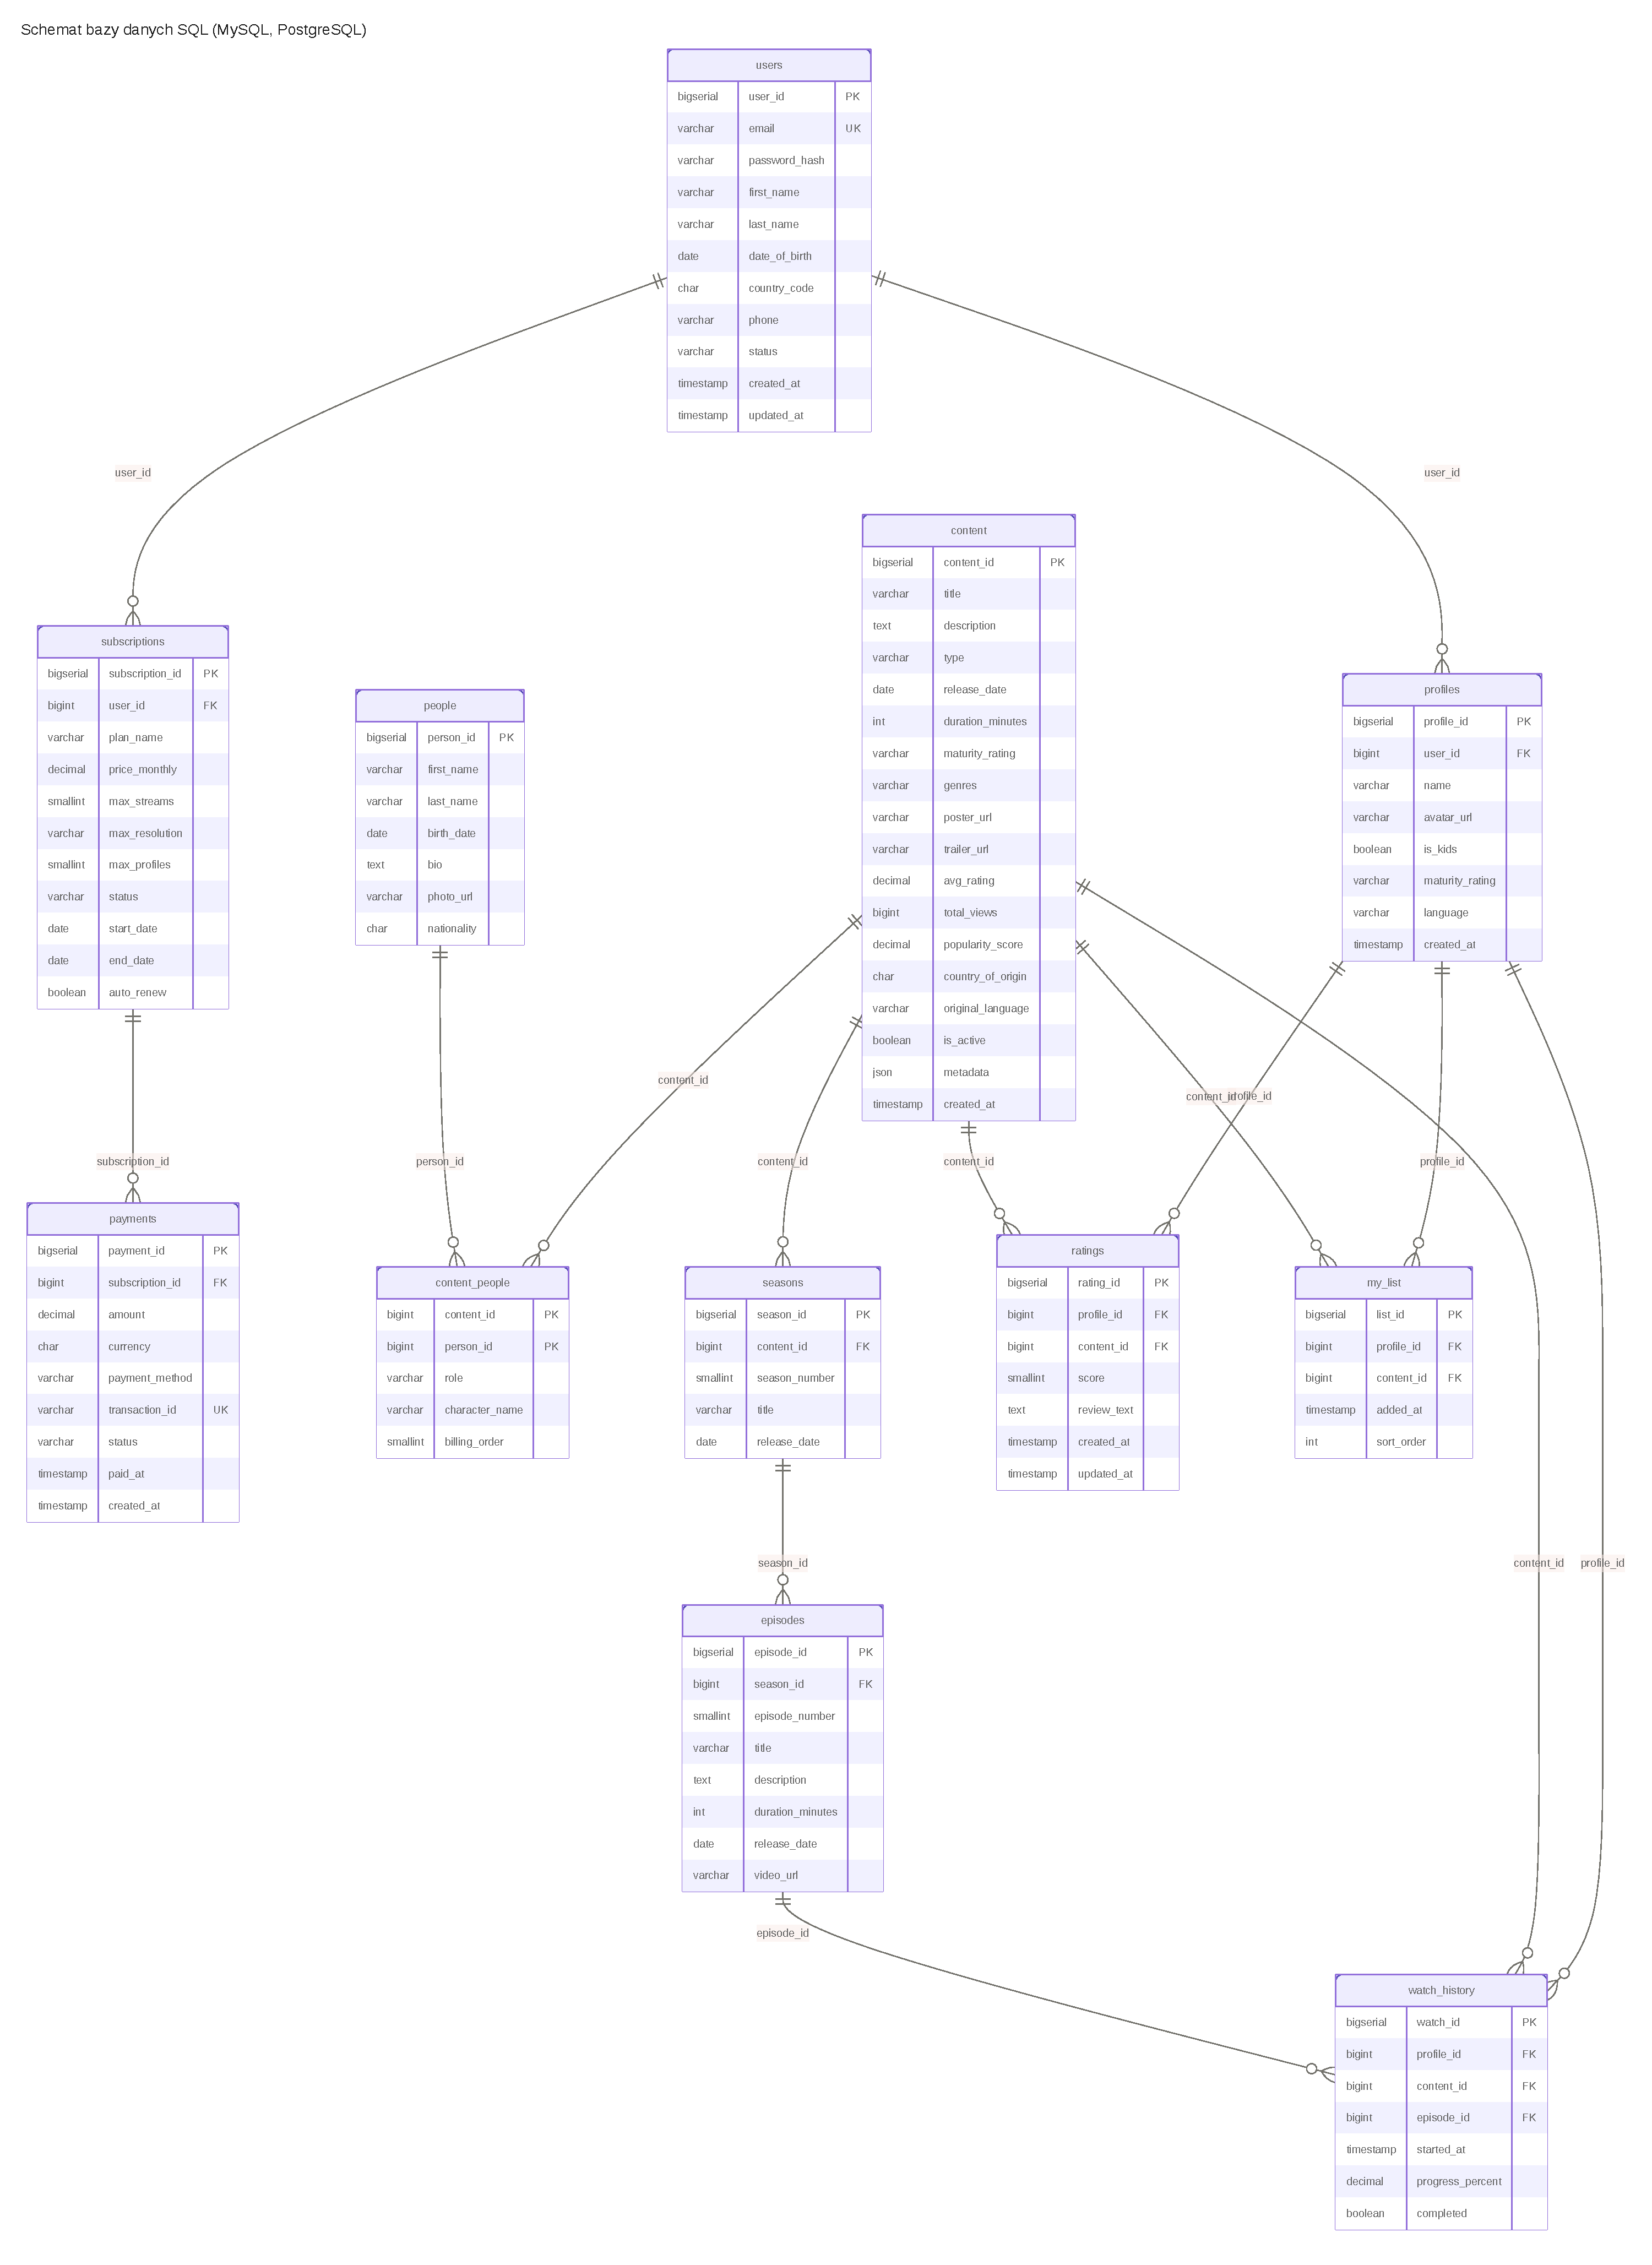
\includegraphics[width=1.0\textwidth]{charts/SchematBazy_SQL.pdf}
    \caption{Schemat relacyjny dla PostgreSQL oraz MySQL}
    \label{fig:schema_sql}
\end{figure}

Domena użytkownika reprezentowana jest przez tabelę \texttt{users}, w której
adres poczty elektronicznej posiada ograniczenie unikalności (\texttt{UNIQUE}),
oraz przez powiązaną z nią relacją jeden-do-wielu tabelę \texttt{profiles},
przechowującą dane poszczególnych profili w obrębie konta. Tabela
\texttt{subscriptions}, również powiązana z \texttt{users} relacją
jeden-do-wielu, rejestruje historię planów subskrypcyjnych wraz z ich
parametrami (cena, dopuszczalna liczba strumieni, maksymalna rozdzielczość).
Tabela \texttt{payments} zawiera informacje o pojedynczych transakcjach
płatniczych powiązanych z konkretną subskrypcją, przy czym pole
\texttt{transaction\_id} podlega ograniczeniu unikalności w celu
wyeliminowania duplikatów.

Domena katalogu treści jest zorganizowana wokół tabeli \texttt{content},
przechowującej zarówno filmy, jak i seriale, rozróżniane przez kolumnę
\texttt{type}. W przypadku seriali strukturę hierarchiczną odwzorowują
tabele \texttt{seasons} oraz \texttt{episodes}, połączone relacjami
jeden-do-wielu odpowiednio z \texttt{content} i \texttt{seasons}. Informacje
o osobach związanych z produkcją -- aktorach, reżyserach oraz scenarzystach --
są utrzymywane w tabeli \texttt{people}, natomiast ich powiązania z konkretnymi
tytułami modeluje tabela łącząca \texttt{content\_people}, realizująca
relację wiele-do-wielu. Klucz główny tej tabeli jest złożony z kolumn
\texttt{content\_id} oraz \texttt{person\_id}, a kolumna \texttt{role}
rozróżnia rodzaj uczestnictwa danej osoby (\textit{director}, \textit{writer},
\textit{actor}). Dla aktorów dodatkowe atrybuty obejmują nazwę odgrywanej
postaci (\texttt{character\_name}) oraz pozycję w napisach
(\texttt{billing\_order}). Gatunki treści zostały zdenormalizowane do postaci
listy w kolumnie \texttt{genres} typu \texttt{varchar}, co stanowi świadomy
kompromis pomiędzy normalizacją a wydajnością odczytu.

Domena aktywności użytkownika obejmuje trzy tabele rejestrujące interakcje
profilu z treścią. Tabela \texttt{watch\_history} przechowuje pojedyncze
sesje odtwarzania wraz z procentowym postępem (\texttt{progress\_percent})
oraz znacznikiem ukończenia (\texttt{completed}); klucze obce wskazują na
\texttt{profiles}, \texttt{content} oraz opcjonalnie \texttt{episodes}
w przypadku seriali. Tabela \texttt{ratings} zawiera oceny treści wystawione
przez profile, w skali liczbowej z możliwą dodatkową recenzją tekstową.
Tabela \texttt{my\_list} reprezentuje listę treści dodanych przez profil
do oglądania w przyszłości, z atrybutem \texttt{sort\_order} określającym
kolejność prezentacji.

Klucze główne wszystkich tabel zostały zaimplementowane jako wartości typu
\texttt{bigserial} (PostgreSQL) lub \texttt{BIGINT AUTO\_INCREMENT} (MySQL),
co zapewnia jednoznaczną identyfikację rekordów oraz monotonicznie rosnącą
sekwencję ułatwiającą wstawianie do indeksów typu B-tree. Klucze obce
zostały opatrzone ograniczeniami referencyjnymi gwarantującymi spójność
danych pomiędzy tabelami. Kolumny \texttt{created\_at} oraz \texttt{updated\_at},
typu \texttt{timestamp}, umożliwiają śledzenie cyklu życia poszczególnych
rekordów.


\subsection{Model dokumentowy (MongoDB)}
Model dokumentowy dla MongoDB stanowi denormalizowane przekształcenie modelu
relacyjnego, dostosowane do typowych wzorców dostępu w aplikacjach
streamingowych. Schemat logiczny obejmuje sześć kolekcji głównych --
\texttt{users}, \texttt{content}, \texttt{watch\_history}, \texttt{ratings},
\texttt{payments} oraz \texttt{my\_list} -- w których część encji powiązanych
relacjami jeden-do-wielu została zagnieżdżona w postaci poddokumentów. Schemat
graficzny przedstawiono na rysunku~\ref{fig:schema_mongo}.

\begin{figure}[H]
    \centering
    % \includegraphics[width=1.0\textwidth]{schemas/schema_mongo.png}
    \caption{Schemat dokumentowy dla MongoDB}
    \label{fig:schema_mongo}
\end{figure}

Kolekcja \texttt{users} agreguje w pojedynczym dokumencie informacje o koncie
użytkownika, tablicę profili (\texttt{profiles[]}) oraz aktualny obiekt
subskrypcji (\texttt{subscription\{\}}). Decyzja o zagnieżdżeniu profili
wynika z faktu, że ich liczba w obrębie konta jest ograniczona (najczęściej
od dwóch do pięciu) oraz że są one praktycznie zawsze pobierane wspólnie
z danymi użytkownika podczas operacji logowania lub przełączania profilu.
Subskrypcja przechowywana jest jako pojedynczy zagnieżdżony obiekt
reprezentujący stan bieżący, podczas gdy historia płatności została
wydzielona do osobnej kolekcji \texttt{payments} z uwagi na rosnący
w czasie wolumen rekordów oraz brak konieczności pobierania ich razem
z danymi użytkownika.

Kolekcja \texttt{content} skupia w pojedynczym dokumencie kompletny opis
filmu lub serialu wraz z zagnieżdżoną tablicą obsady (\texttt{cast[]}) oraz,
w przypadku seriali, dwupoziomową hierarchią sezonów i odcinków
(\texttt{seasons[]} zawierającą \texttt{episodes[]}). Tablica obsady
przechowuje denormalizowaną kopię podstawowych danych każdej osoby --
imię, nazwisko, rolę oraz, dla aktorów, nazwę postaci i pozycję w napisach --
co eliminuje konieczność wykonywania operacji \texttt{\$lookup} przy
typowym scenariuszu pobrania szczegółów tytułu. Gatunki przechowywane są
jako tablica wartości tekstowych (\texttt{genres[]}), co umożliwia
wykorzystanie indeksu wielowartościowego (\textit{multikey index}) do
efektywnego wyszukiwania treści po wybranej kategorii. Pole \texttt{metadata},
typu \texttt{object}, agreguje dodatkowe atrybuty marketingowe i techniczne,
omówione szczegółowo w kolejnym podrozdziale.

Kolekcje rejestrujące aktywność użytkownika -- \texttt{watch\_history},
\texttt{ratings} oraz \texttt{my\_list} -- zostały utrzymane jako odrębne
struktury, mimo że w modelu hierarchicznym stanowiłyby naturalne kandydatury
do zagnieżdżenia w obrębie dokumentu profilu. Decyzja o ich wydzieleniu
wynika z dwóch przesłanek: rosnącego w czasie wolumenu rekordów, który
w przypadku zagnieżdżenia mógłby przekroczyć limit szesnastu megabajtów
przypadający na pojedynczy dokument BSON, oraz konieczności efektywnego
wyszukiwania po identyfikatorze treści, na przykład w celu wyznaczenia
średniej oceny lub liczby unikalnych widzów dla danego tytułu. Powiązania
z dokumentami nadrzędnymi realizowane są przez referencje
(\texttt{profile\_id}, \texttt{content\_id}), z indeksami złożonymi
zaprojektowanymi pod konkretne wzorce zapytań -- typowo
\texttt{(profile\_id, started\_at)} dla historii oglądania oraz
\texttt{(content\_id, score)} dla ocen.

Kolekcja \texttt{payments} została wydzielona z dokumentu użytkownika,
ponieważ liczba transakcji per subskrypcja może być znacząca, a dane te
są przetwarzane głównie w zapytaniach analitycznych (raporty przychodów,
analiza skuteczności metod płatności), niezwiązanych bezpośrednio
z operacjami na koncie użytkownika. Powiązanie z subskrypcją realizowane
jest przez referencję \texttt{subscription\_id}, mapującą się na identyfikator
zagnieżdżony w dokumencie \texttt{users}.

Pole \texttt{\_id} stanowi domyślny identyfikator każdego dokumentu, na
którym automatycznie zakładany jest unikalny indeks. Dla zachowania
kompatybilności semantycznej z modelem relacyjnym zachowano typ
\texttt{bigserial} (mapowany na 64-bitową liczbę całkowitą), zamiast
domyślnego typu \texttt{ObjectId}, co ułatwia generowanie identyfikatorów
zewnętrznym skryptem oraz zapewnia bezpośrednią porównywalność z modelami
SQL podczas testów wydajnościowych.


\subsection{Model grafowy (Neo4j)}
Model grafowy dla Neo4j stanowi najistotniejsze odwzorowanie domeny problemu
spośród trzech analizowanych podejść, ponieważ relacje między encjami zostały
podniesione do rangi obiektów pierwszej klasy. Schemat składa się z dziewięciu
typów węzłów oraz dwunastu typów relacji, ze szczególnym uwzględnieniem
właściwości przypisywanych krawędziom. Strukturę przedstawiono na
rysunku~\ref{fig:schema_neo4j}.

\begin{figure}[H]
    \centering
    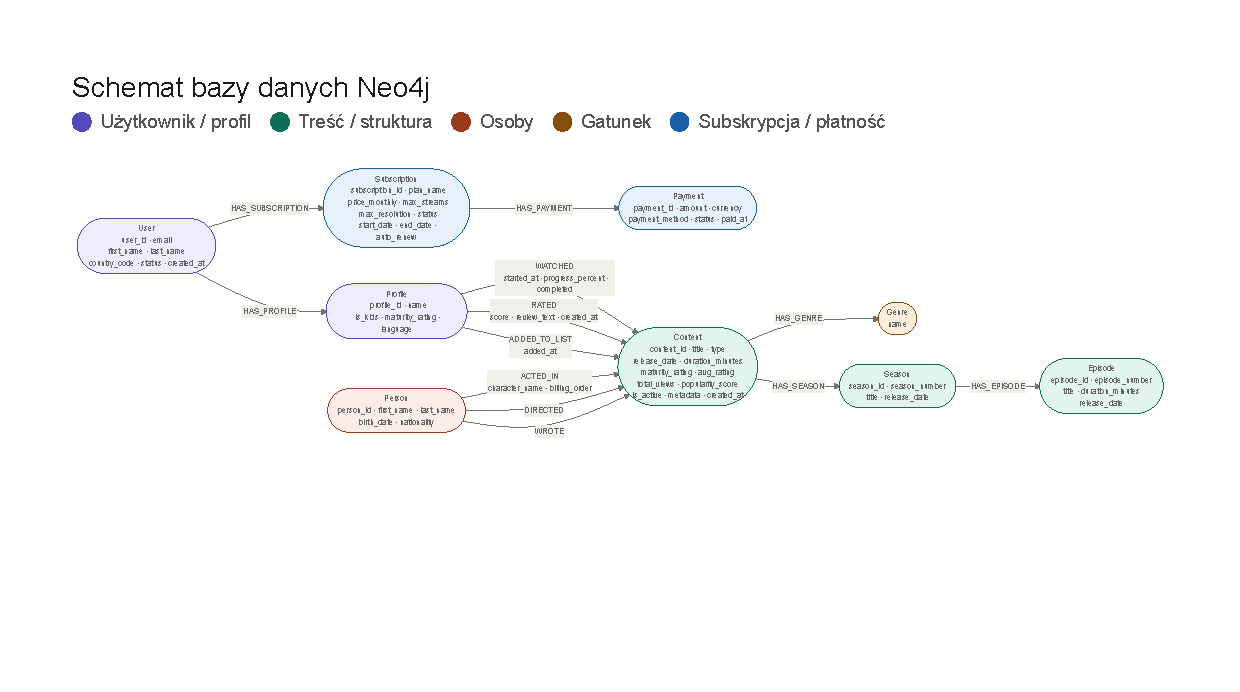
\includegraphics[width=1.0\textwidth]{charts/SchematBazy_neo4j_cropped.pdf}
    \caption{Schemat grafowy dla Neo4j}
    \label{fig:schema_neo4j}
\end{figure}

Domena użytkownika reprezentowana jest przez węzły \texttt{User} oraz
\texttt{Profile}, połączone relacją \texttt{HAS\_PROFILE}. Subskrypcja
została wymodelowana jako odrębny węzeł \texttt{Subscription} powiązany
z użytkownikiem relacją \texttt{HAS\_SUBSCRIPTION}, natomiast historia
płatności obejmuje węzły \texttt{Payment} podpięte do odpowiadających im
subskrypcji relacją \texttt{HAS\_PAYMENT}. Wybór reprezentacji subskrypcji
oraz płatności jako pełnoprawnych węzłów, a nie właściwości użytkownika,
umożliwia efektywne realizowanie zapytań analitycznych, takich jak
identyfikacja użytkowników z aktywną subskrypcją typu \textit{Premium}
lub agregacja przychodów według metody płatności w ustalonym oknie czasowym.

Domena katalogu treści jest zorganizowana wokół centralnego węzła
\texttt{Content}, łączącego się z hierarchią węzłów \texttt{Season} oraz
\texttt{Episode} poprzez relacje \texttt{HAS\_SEASON} oraz
\texttt{HAS\_EPISODE}. Gatunki zostały wymodelowane jako odrębne węzły
\texttt{Genre} powiązane z treścią relacją \texttt{HAS\_GENRE} -- struktura
ta umożliwia efektywne wyszukiwanie treści powiązanych wspólnym gatunkiem
oraz analizę popularności poszczególnych kategorii bez konieczności
skanowania pełnego katalogu. Osoby uczestniczące w produkcji reprezentowane
są przez węzły \texttt{Person}, połączone z węzłami \texttt{Content} przez
trzy odrębne typy relacji: \texttt{ACTED\_IN}, \texttt{DIRECTED} oraz
\texttt{WROTE}. Rozdzielenie ról na osobne typy relacji, zamiast zakodowania
ich jako właściwości pojedynczej krawędzi, umożliwia precyzyjne kierowanie
zapytań oraz wykorzystanie wbudowanej optymalizacji silnika dla konkretnego
typu krawędzi.

Domena aktywności użytkownika została w całości odwzorowana przez relacje
łączące węzły \texttt{Profile} z węzłami \texttt{Content}. Relacja
\texttt{WATCHED} reprezentuje sesje odtwarzania i posiada właściwości
\texttt{started\_at}, \texttt{progress\_percent} oraz \texttt{completed},
przeniesione z tabeli \texttt{watch\_history} modelu relacyjnego. Relacja
\texttt{RATED} przechowuje oceny treści wraz z ich wartością liczbową
(\texttt{score}), opcjonalnym tekstem recenzji (\texttt{review\_text}) oraz
znacznikiem czasu (\texttt{created\_at}). Lista treści dodanych przez
profil reprezentowana jest przez relację \texttt{ADDED\_TO\_LIST}
z właściwością \texttt{added\_at}. Reprezentacja tych encji jako relacji
zamiast węzłów wynika z faktu, że nie posiadają one istotnej tożsamości
poza powiązaniem dwóch obiektów -- profilu oraz treści.

Analogicznie do relacji aktywności, relacja \texttt{ACTED\_IN} przechowuje
właściwości \texttt{character\_name} oraz \texttt{billing\_order}, charakteryzujące
konkretną rolę aktorską, a nie samą osobę. Pozwala to na zwięzłe wyrażanie
zapytań typu „znajdź wszystkich aktorów grających pierwsze role w filmach
nominowanych do określonej nagrody" w pojedynczym wzorcu Cypher,
unikającym wielokrotnych operacji złączenia.

Identyfikatory zewnętrzne zostały zachowane jako właściwości węzłów
(\texttt{user\_id}, \texttt{content\_id} i analogiczne), niezależnie od
wewnętrznych identyfikatorów silnika Neo4j, co umożliwia bezpośrednią
porównywalność danych pomiędzy modelami w trakcie testów wydajnościowych.
Indeksy zostały założone na właściwościach wykorzystywanych w warunkach
filtrujących typowych zapytań -- \texttt{User.email}, \texttt{Content.title},
\texttt{Content.type} oraz \texttt{Person.last\_name} -- co umożliwia silnikowi
zlokalizowanie punktu startowego trawersu grafu w czasie logarytmicznym.


\subsection{Dane półstrukturalne (JSON/JSONB)}
Każda z czterech analizowanych baz danych obsługuje dane półstrukturalne
w postaci dokumentów JSON, lecz robi to w sposób różniący się zarówno
implementacją, jak i konsekwencjami wydajnościowymi. W modelu danych platformy
streamingowej zostało celowo wykorzystane pole \texttt{metadata} w tabeli
\texttt{content}, przechowujące dodatkowe atrybuty marketingowe oraz
techniczne, które nie stanowią naturalnych kandydatów do reprezentacji
kolumnowej. Pole to obejmuje informacje o studiu produkcyjnym, budżecie,
otrzymanych nagrodach, znacznikach kategoryzujących, krajach koprodukcji
oraz parametrach jakościowych strumienia (maksymalna rozdzielczość, wsparcie
HDR, obsługa Dolby Atmos), które łącznie tworzą strukturę zagnieżdżoną
o zmiennej liczbie pól.

\textbf{PostgreSQL} udostępnia dwa typy danych dokumentowych: \texttt{json}
oraz \texttt{jsonb}. Pierwszy z nich zachowuje dokument w postaci tekstowej,
co skutkuje koniecznością ponownego parsowania przy każdej operacji odczytu,
natomiast \texttt{jsonb} przechowuje dokument w postaci binarnej, znormalizowanej
strukturze drzewa, eliminując narzut parsowania oraz umożliwiając efektywne
indeksowanie. W omawianym modelu pole \texttt{metadata} zostało zadeklarowane
jako \texttt{jsonb}, co pozwala na wykorzystanie pełnego zestawu operatorów
ścieżkowych: \texttt{->} (dostęp do pola jako JSON), \texttt{->>} (dostęp
do pola jako tekst), \texttt{@>} (sprawdzenie zawierania) oraz wyrażeń
\texttt{jsonpath} wprowadzonych w wersji 12. Najistotniejszą zaletą
PostgreSQL w kontekście danych półstrukturalnych pozostaje wsparcie dla
indeksów GIN, umożliwiających efektywne filtrowanie po dowolnych polach
dokumentu. Indeks GIN założony na całym dokumencie pozwala na realizację
zapytań typu „znajdź treści posiadające określony znacznik" bez konieczności
sekwencyjnego skanowania tabeli, natomiast indeks częściowy GIN wykorzystujący
wyrażenie \texttt{jsonb\_path\_ops} ogranicza rozmiar indeksu w sytuacji,
gdy wymagany jest wyłącznie operator zawierania.

\textbf{MySQL} obsługuje dane półstrukturalne poprzez natywny typ
\texttt{JSON}, dostępny od wersji 5.7. Implementacja zachowuje dokument
w wewnętrznej postaci binarnej zbliżonej do BSON, co eliminuje konieczność
parsowania tekstowego przy odczycie. Dostęp do pól realizowany jest przez
operatory \texttt{->} oraz \texttt{->>}, składniowo zgodne z PostgreSQL,
oraz przez funkcje \texttt{JSON\_EXTRACT}, \texttt{JSON\_VALUE} i
\texttt{JSON\_TABLE}. Zasadniczym ograniczeniem MySQL pozostaje brak
możliwości bezpośredniego indeksowania pól dokumentu JSON. Aby umożliwić
efektywne filtrowanie po wybranym atrybucie, należy zdefiniować kolumnę
generowaną (\texttt{GENERATED ALWAYS AS}) wyznaczającą wartość konkretnego
pola JSON, a następnie założyć na niej standardowy indeks B-tree. W modelu
omawianej platformy przykładem takiego rozwiązania jest indeks na kolumnie
generowanej wyznaczającej wartość pola \texttt{metadata.studio}, umożliwiający
szybkie filtrowanie treści według studia produkcyjnego. Rozwiązanie to,
choć funkcjonalne, jest wyraźnie mniej elastyczne niż mechanizm GIN
oferowany przez PostgreSQL, wymaga bowiem deklaratywnego określenia
indeksowanych pól na etapie projektowania schematu.

\textbf{MongoDB} traktuje dokumenty jako podstawowy model danych, co
eliminuje pojęcie dedykowanego typu JSON -- każda kolekcja przechowuje
dokumenty BSON o dowolnej strukturze. Pole \texttt{metadata} stanowi
zagnieżdżony obiekt, indeksowany w sposób analogiczny do pól zwykłych --
bezpośrednio przez ścieżkę kropkową, na przykład\\
\texttt{db.content.createIndex(\{"metadata.studio": 1\})}. Indeksy
wielokluczowe (\textit{multikey indexes}) są zakładane automatycznie dla
pól o wartości tablicowej, takich jak \texttt{metadata.tags}, co pozwala
na efektywne filtrowanie treści zawierających konkretny znacznik. Dla
zapytań po wielu polach jednocześnie dostępne są indeksy złożone, a dla
wyszukiwania pełnotekstowego w obrębie dokumentu -- indeksy tekstowe
oraz, w platformie Atlas, mechanizm Atlas Search oparty na bibliotece
Apache Lucene. W zestawieniu z silnikami relacyjnymi MongoDB oferuje
najbardziej naturalne i bezpośrednie wsparcie dla danych zagnieżdżonych,
za cenę utraty części gwarancji modelu relacyjnego, takich jak referencje
między dokumentami egzekwowane przez silnik.

\textbf{Neo4j} nie operuje typem JSON jako odrębnym typem danych --
właściwości węzłów oraz relacji są pojedynczymi wartościami skalarnymi
lub tablicowymi, lecz nie mogą posiadać dowolnej zagnieżdżonej struktury.
W konsekwencji pola, które w modelach SQL oraz dokumentowym znajdowały się
wewnątrz dokumentu \texttt{metadata}, w modelu grafowym zostały
przedstawione w postaci osobnych właściwości węzła \texttt{Content}
(\texttt{studio}, \texttt{budget}, \texttt{max\_resolution},
\texttt{hdr\_supported}, \texttt{dolby\_atmos}) lub, w przypadku list,
w postaci osobnych węzłów połączonych relacjami (na przykład węzły
\texttt{Award} mogłyby zostać połączone z \texttt{Content} relacją
\texttt{WON\_AWARD}). Biblioteka APOC udostępnia procedury
\texttt{apoc.convert.fromJsonMap} oraz \texttt{apoc.load.json}, umożliwiające
import dokumentów JSON do struktury grafowej, lecz natywny silnik Neo4j
nie przechowuje dokumentów w postaci dokumentowej.

Z porównania powyższych implementacji wynika, że PostgreSQL oraz MongoDB
oferują najbogatsze wsparcie dla danych półstrukturalnych, przy czym
PostgreSQL zachowuje dodatkowo pełen rygor relacyjny i transakcyjny,
natomiast MongoDB pozwala na operowanie dokumentami w sposób najbardziej
bezpośredni. MySQL oferuje funkcjonalność porównywalnie ograniczoną do
podstawowego dostępu i wymaga ręcznej dekompozycji indeksowanych pól,
natomiast Neo4j wymusza częściowe spłaszczenie struktury w fazie
projektowania schematu. Wybór reprezentacji pola \texttt{metadata} stanowi
zatem nie tylko decyzję modelową, lecz również istotny czynnik wpływający
na charakterystykę wydajnościową poszczególnych silników, co znalazło
odzwierciedlenie w doborze scenariuszy testowych.


\subsection{Generacja danych}
Dane testowe zostały wygenerowane przy pomocy autorskiego skryptu napisanego
w języku Python, zlokalizowanego w module \texttt{src/generators/data\_generator.py}.
Generator korzysta z biblioteki Faker w wersji obsługującej lokalizacje
\texttt{pl\_PL} oraz \texttt{en\_US}, co umożliwia tworzenie realistycznych
danych osobowych z mieszanką polskich i anglojęzycznych imion, nazwisk oraz
opisów tekstowych. Wszystkie generowane wartości pseudolosowe są
deterministycznie powtarzalne dzięki ustawieniu wspólnego ziarna (\texttt{seed=42})
zarówno dla biblioteki Faker, jak i dla wbudowanego generatora liczb
losowych Pythona, co gwarantuje powtarzalność wyników testów wydajnościowych
pomiędzy uruchomieniami.

Konfiguracja wolumenu danych została zdefiniowana w module \texttt{src/config.py}
w postaci trzech profili: \textit{small}, \textit{medium} oraz \textit{large}.
Profil small obejmuje 5\,000 użytkowników, 2\,000 osób w katalogu twórców,
2\,000 tytułów oraz 300\,000 sesji oglądania. Profil medium zawiera
odpowiednio 20\,000 użytkowników, 5\,000 osób, 5\,000 tytułów oraz 500\,000
sesji oglądania. Profil large powiększa zbiór do 100\,000 użytkowników,
20\,000 osób, 15\,000 tytułów oraz 6\,000\,000 sesji oglądania. Łączna liczba
rekordów we wszystkich tabelach docelowo osiąga około pół miliona, miliona
oraz dziesięciu milionów wierszy odpowiednio dla wolumenów small, medium
oraz large, co umożliwia obserwację skalowania charakterystyk wydajnościowych
silników względem rozmiaru zbioru.

W pierwszym etapie generacji danych tworzone są encje
niezależne -- użytkownicy, osoby z katalogu twórców oraz treści. Następnie
generowane są encje powiązane jeden-do-wielu z użytkownikiem (profile,
subskrypcje oraz płatności), encje powiązane z treścią (powiązania
z osobami, sezony, odcinki) oraz, w ostatnim etapie, rekordy aktywności
profili (historia oglądania, lista do obejrzenia, oceny). Każda tabela
zapisywana jest w postaci osobnego pliku CSV z kodowaniem UTF-8, co
umożliwia jednolity import do wszystkich czterech systemów bazodanowych.

Procedura generowania użytkowników wprowadza realistyczne rozkłady
prawdopodobieństwa odzwierciedlające typową dystrybucję rynkową. Kraj
zamieszkania jest losowany z wagą 40\% dla Polski, 15\% dla Stanów
Zjednoczonych oraz mniejszymi udziałami pozostałych ośmiu krajów
europejskich. Numer telefonu jest poprzedzany prefiksem zgodnym z krajem
i jest obecny u około 70\% użytkowników. Status konta jest losowany
z rozkładu, w którym użytkownicy aktywni stanowią dominującą większość,
przy czym uwzględniono również kategorie \textit{inactive}, \textit{suspended}
oraz \textit{deleted}, co pozwala na realistyczne modelowanie zapytań
filtrujących po stanie konta. Adresy e-mail konstruowane są na podstawie
imienia, nazwiska oraz identyfikatora użytkownika, z wykorzystaniem zbioru
typowych domen polskich i międzynarodowych. Wartość pola
\texttt{password\_hash} jest pseudolosowym ciągiem znaków zgodnym
z formatem skrótu bcrypt.

Liczba profili przypadających na konto jest losowana z rozkładu, w którym
najczęstsza wartość mieści się w przedziale od dwóch do trzech profili,
co odpowiada typowemu wzorcowi użycia rodzinnego. Profil drugi w obrębie
konta jest oznaczany jako profil dziecięcy z prawdopodobieństwem 40\%,
co automatycznie ustawia jego klasyfikację wiekową na wartość \textit{ALL}.
Liczba subskrypcji per użytkownik również jest losowana z odpowiedniego
rozkładu, przy czym ostatnia subskrypcja zawsze posiada status
\textit{active}, natomiast wcześniejsze są oznaczane jako \textit{cancelled}
lub \textit{expired}, co umożliwia testowanie zapytań analizujących historię
zmian planu. Plan subskrypcji wybierany jest spośród trzech wariantów --
\textit{Basic}, \textit{Standard} oraz \textit{Premium} -- z wagami 30\%,
45\% oraz 25\% odpowiednio.

Treści są dzielone na filmy oraz seriale w stosunku 60\% do 40\%. Filmy
posiadają określoną długość, natomiast seriale otrzymują strukturę
podrzędną w postaci sezonów oraz odcinków. Liczba sezonów na serial
podlega rozkładowi malejącemu, w którym dominują seriale jedno-,
dwu- oraz trzysezonowe. Liczba odcinków w sezonie jest losowana
z przedziału od czterech do szesnastu, z datami premier rozłożonymi
w cotygodniowych odstępach. Każdy tytuł otrzymuje od jednej do trzech
etykiet gatunkowych losowanych z dwunastoelementowego zbioru.

Dla każdego tytułu generowany jest również obiekt JSON wypełniający
pole \texttt{metadata}. Obiekt zawiera nazwę studia produkcyjnego,
budżet w przedziale od 500\,000 do 200\,000\,000 jednostek, listę
otrzymanych nagród (od zera do trzech pozycji), listę znaczników
kategoryzujących, listę krajów koprodukcji oraz zagnieżdżony obiekt
\texttt{streaming\_quality} z parametrami technicznymi strumienia.
Tak skonstruowane pole umożliwia testowanie scenariuszy odpytywania
danych zagnieżdżonych w sposób reprezentatywny dla rzeczywistych
zastosowań platform streamingowych.

Powiązania między treściami a osobami są generowane z zachowaniem
struktury produkcyjnej -- każdy tytuł otrzymuje dokładnie jednego
reżysera, od jednego do dwóch scenarzystów oraz od trzech do dwunastu
aktorów, każdy z przypisaną nazwą postaci oraz pozycją w napisach.
Sesje oglądania są przypisywane losowym profilom oraz losowym treściom,
przy czym dla seriali wybierany jest losowy odcinek z dostępnych. Postęp
oglądania jest losowany z rozkładu jednostajnego od zera do stu procent,
a wartości przekraczające próg 95\% są normalizowane do stu procent
i oznaczane znacznikiem ukończenia. Oceny wystawiane przez profile
podlegają rozkładowi pochylonemu w stronę wartości pozytywnych
(z modą w przedziale od siedmiu do ośmiu punktów), co odzwierciedla
typową asymetrię ocen obserwowaną na platformach streamingowych.
Tekst recenzji jest dołączany w 30\% przypadków.

Wygenerowane pliki CSV stanowią wspólny punkt wyjścia dla mechanizmów
ładowania danych do każdego z czterech systemów bazodanowych. Konwersja
do modelu dokumentowego MongoDB realizowana jest przez dedykowany skrypt
importujący, który łączy plik \texttt{users.csv} z plikami \texttt{profiles.csv}
oraz \texttt{subscriptions.csv} w pojedynczy dokument oraz osadza dane
gatunków, obsady, sezonów i odcinków wewnątrz dokumentów kolekcji
\texttt{content}. Konwersja do modelu grafowego Neo4j realizowana jest
narzędziem \texttt{neo4j-admin import}, które przyjmuje pliki CSV
opisujące węzły oraz relacje w formacie zgodnym ze specyfikacją silnika.
Mechanizmy ładowania danych dla poszczególnych silników zostały szczegółowo
opisane w dalszej części pracy.


% -------------------------------------------------------
\section{Środowisko testowe}
\subsection{Docker Compose i konfiguracja silników}

Środowisko testowe zostało sprowadzone do jednego pliku \texttt{docker-compose.yml}
definiującego cztery izolowane kontenery -- po jednym na każdy z porównywanych silników
bazodanowych. Pozwoliło to uzyskać pełną reprodukowalność (każde uruchomienie
startuje z identycznego obrazu), czyste odseparowanie procesów (żaden silnik nie
dzieli RAM-u innym) oraz jednolity interfejs startu i zatrzymania
całego stosu jedną komendą \texttt{docker compose up}.

Każdy kontener ma jawnie ustawiony limit pamięci (\texttt{deploy.resources.limits.memory})
oraz własne, świadomie dobrane opcje tuningowe -- tak aby zapewnić porównywalne
warunki pracy bez nieuczciwego faworyzowania żadnej z baz.
Wszystkie kontenery udostępniają swoje porty
(\texttt{5432}, \texttt{3306}, \texttt{27017}, \texttt{7687}+\texttt{7474}),
dzięki czemu warstwa orkiestracji w Pythonie łączy się do nich przez \texttt{localhost}.
Dane są utrzymywane  w czterech nazwanych wolumenach Docker (\texttt{postgres\_data},
\texttt{mysql\_data}, \texttt{mongo\_data}, \texttt{neo4j\_data}), co pozwala zachować
załadowaną bazę między kolejnymi uruchomieniami benchmarków.

\subsubsection*{PostgreSQL 17}

Kontener \texttt{ztbd-postgres} oparty o obraz \texttt{postgres:17} z limitem 2~GB
RAM. Schemat bazy (12 tabel wraz z kluczami obcymi i kaskadami jest ładowany automatycznie przy pierwszym starcie
kontenera, poprzez zamontowanie pliku \texttt{init.sql} w katalogu
\texttt{/docker-entrypoint-initdb.d/}. Parametry uruchomieniowe silnika:

\begin{lstlisting}[language=bash,basicstyle=\ttfamily\small]
shared_buffers=512MB
work_mem=16MB
maintenance_work_mem=512MB
effective_cache_size=1536MB
wal_buffers=16MB
checkpoint_completion_target=0.9
max_wal_size=2GB
synchronous_commit=off
\end{lstlisting}

\subsubsection*{MySQL 8.0}
Kontener \texttt{ztbd-mysql} oparty o obraz \texttt{mysql:8.0}, również z limitem
2~GB RAM i własnym \texttt{init.sql}. Parametry silnika InnoDB:

\begin{lstlisting}[language=bash,basicstyle=\ttfamily\small]
--innodb-buffer-pool-size=1073741824    (1 GB)
--innodb-log-file-size=256M
--innodb-flush-log-at-trx-commit=2
--innodb-flush-method=O_DIRECT
--innodb-doublewrite=0
--innodb-change-buffering=all
--bulk-insert-buffer-size=256M
--local-infile=1
--max-allowed-packet=256M
--innodb-autoinc-lock-mode=2
\end{lstlisting}


\subsubsection*{MongoDB 8.0}

Kontener \texttt{ztbd-mongo} oparty o obraz \texttt{mongo:8.0}, limit 2~GB RAM,
port \texttt{27017}. Konfiguracja silnika WiredTiger sprowadza się do jednej,
ale kluczowej opcji:

\begin{lstlisting}[language=bash,basicstyle=\ttfamily\small]
mongod --wiredTigerCacheSizeGB 1.2
\end{lstlisting}

\noindent 1.2~GB to 60\% limitu kontenera -- rozmiar cache silnika pamięciowego
WiredTiger, w którym MongoDB trzyma skompresowane strony dokumentów i indeksów.
Pozostałe 40\% pozostawione jest na procesy Mongo poza cache (połączenia, sortowanie,
agregacje, heap). Schemat nie jest ładowany -- Mongo nie wymaga definicji kolekcji
z góry, tworzą się one przy pierwszym zapisie.

\subsubsection*{Neo4j 2026.02.2}

Kontener \texttt{ztbd-neo4j} oparty o obraz \texttt{neo4j:2026.02.2} (najnowsza
wersja z aktywną linią wsparcia) z doinstalowanym pluginem \textbf{APOC}.
Ze wszystkich
czterech baz Neo4j dostał \textbf{najwyższy limit pamięci -- 4~GB} -- ze względu
na architekturę opartą o JVM, która wymaga osobnego budżetu na heap, osobnego
na page cache plików bazy oraz osobnego na pamięć transakcyjną:

\begin{lstlisting}[language=bash,basicstyle=\ttfamily\small]
server.memory.heap.initial_size      = 1g
server.memory.heap.max_size          = 1g
server.memory.pagecache.size         = 1g
dbms.memory.transaction.total.max    = 3g
\end{lstlisting}


% -------------------------------------------------------
\subsection{Technologie i biblioteki}

Warstwa orkiestracji (generowanie danych, ładowanie, benchmarki, \texttt{EXPLAIN},
wizualizacja) została zaimplementowana w \textbf{Pythonie 3.12+}. Wybór Pythona
wynika z dostępności natywnych, dojrzałych driverów do wszystkich czterech silników,
bogatego ekosystemu narzędzi analitycznych (\texttt{pandas}, \texttt{matplotlib})
oraz niskiego narzutu zapisu kodu -- zestaw 24~scenariuszy da się zwięźle wyrazić
w języku wysokiego poziomu, bez zaciemniania logiki pomiaru ogólnikami języka.

Cały projekt jest uruchamiany przez jeden punkt wejścia (\texttt{main.py}) udostępniający
sześć komend CLI zbudowanych na module \texttt{argparse}: \texttt{generate},
\texttt{load}, \texttt{benchmark}, \texttt{explain}, \texttt{visualize} oraz
\texttt{run-all} (pełny pipeline 8-krokowy: generowanie~$\rightarrow$~ładowanie
bez indeksów~$\rightarrow$~benchmarki~$\rightarrow$~\texttt{EXPLAIN}~$\rightarrow$~ładowanie
z indeksami~$\rightarrow$~benchmarki z indeksami~$\rightarrow$~\texttt{EXPLAIN} z
indeksami~$\rightarrow$~wizualizacja).

\subsubsection*{Drivery bazodanowe}

\begin{itemize}
    \item \textbf{psycopg 3} -- PostgreSQL. Najnowszy driver, obsługujący operacje asynchroniczne  
    protokół \texttt{COPY FROM STDIN} strumieniowo,
    co jest kluczowe dla wydajnego ładowania danych.
    \item \textbf{PyMySQL} -- MySQL. Driver napisany w czystym Pythonie (bez zależności na
    \texttt{mysqlclient} wymagającym kompilacji); wspiera \texttt{LOAD DATA LOCAL INFILE}
    poprzez flagę \texttt{local\_infile=True} w \texttt{connect()}.
    \item \textbf{PyMongo} -- MongoDB. Oficjalny driver do MongoDB; wspiera
    \texttt{insert\_many(ordered=False)} (kontynuacja po błędach duplikatów) oraz
    korzystanie z zaawansowanych zapytań typu \texttt{aggregate}.
    \item \textbf{neo4j} (oficjalny driver Pythonowy) -- Neo4j. Komunikacja przez
    protokół Bolt na porcie 7687; kluczowe jest tu wykorzystywanie jednej sesji
    (\texttt{driver.session()}) dla wielu operacji -- żeby uniknąć narzutu połączeń TCP przy każdym batchu.
\end{itemize}

\subsubsection*{Generowanie danych}

Generator danych (\texttt{src/generators/data\_generator.py}) opiera się na
bibliotece \textbf{Faker} z \textbf{ustalonym seedem 42}.
Stały seed gwarantuje pełną powtarzalność -- każde wywołanie
\texttt{python main.py generate --volume small} produkuje identyczny
zestaw plików CSV, co jest niezbędne dla rzetelności porównania (wszystkie cztery bazy
dostają dokładnie te same dane wejściowe). Wyjściem są pliki CSV
(po jednym na tabelę), które każdy z czterech loaderów czyta niezależnie
i transformuje do swojej natywnej reprezentacji.

\subsubsection*{Analiza i wizualizacja}

Warstwa analityczna korzysta z trzech standardowych bibliotek:

\begin{itemize}
    \item \textbf{pandas} -- wczytywanie plików CSV z wynikami, agregacje
    (\texttt{groupby} po scenariuszu, bazie, wariancie indeksów), obliczanie
    mediany, min i max z 3 triali.
    \item \textbf{NumPy} -- operacje macierzowe przy liczeniu heatmap.
    \item \textbf{matplotlib} (backend \texttt{Agg}) -- generowanie wykresów PNG
    bez wymagania GUI.
\end{itemize}




% -------------------------------------------------------
\section{Ładowanie danych i indeksy}
\subsection{Metody ładowania danych}
\subsection{Typy indeksów i strategia indeksowania}

% -------------------------------------------------------
\section{Metodologia benchmarków}
\subsection{Cold start i cachowanie}
\subsection{Pipeline testowy}

% -------------------------------------------------------
\section{Scenariusze testowe}
\subsection{INSERT (I1--I6)}

Grupa scenariuszy INSERT obejmuje sześć wariantów wstawiania danych -- od pojedynczego
rekordu z powiązaniami, przez masowe ładowanie paczek rekordów, aż po wstawianie złożonych struktur
hierarchicznych. Scenariusze różnią się
wolumenem wstawianych danych oraz stopniem powiązań między rekordami, co pozwala
porównać efektywność mechanizmów masowego ładowania w każdym z silników (COPY,
multi-row INSERT, \texttt{insertMany}, \texttt{UNWIND + CALL IN TRANSACTIONS}) oraz
koszt utrzymania spójności relacyjnej i referencyjnej przy zapisie.

\subsubsection{I1: Rejestracja użytkownika}

Rejestracja nowego użytkownika platformy -- w ramach jednej operacji tworzony
jest rekord użytkownika, jego domyślny profil oraz aktywna subskrypcja w planie
Standard. Scenariusz testuje koszt wstawienia powiązanych rekordów w trzech
różnych tabelach/kolekcjach/węzłach grafu oraz utrzymania ich spójności
(relacja 1-1 users→subscription, 1-N users→profiles).

\textbf{PostgreSQL}
\begin{lstlisting}[language=SQL]
INSERT INTO users (email, password_hash, first_name, last_name,
    date_of_birth, country_code, status, created_at, updated_at)
VALUES (%s, '$2b$12$benchmark', 'Bench', 'User',
    '1990-01-01', 'PL', 'active', NOW(), NOW())
RETURNING user_id;

INSERT INTO profiles (user_id, name, maturity_rating, language, created_at)
VALUES (%s, 'Main', 'ALL', 'pl', NOW());

INSERT INTO subscriptions (user_id, plan_name, price_monthly, max_streams,
    max_resolution, status, start_date, auto_renew, created_at)
VALUES (%s, 'Standard', 43.99, 2, '1080p', 'active', CURRENT_DATE, TRUE, NOW());
\end{lstlisting}

\textbf{MySQL}
\begin{lstlisting}[language=SQL]
INSERT INTO users (email, password_hash, first_name, last_name,
    date_of_birth, country_code, status, created_at, updated_at)
VALUES (%s, '$2b$12$benchmark', 'Bench', 'User',
    '1990-01-01', 'PL', 'active', NOW(), NOW());

INSERT INTO profiles (user_id, name, maturity_rating, language, created_at)
VALUES (%s, 'Main', 'ALL', 'pl', NOW());

INSERT INTO subscriptions (user_id, plan_name, price_monthly, max_streams,
    max_resolution, status, start_date, auto_renew, created_at)
VALUES (%s, 'Standard', 43.99, 2, '1080p', 'active', CURDATE(), TRUE, NOW());
\end{lstlisting}

\textbf{MongoDB}
\begin{lstlisting}[language=Python]
db.users.insertOne({
    _id: <uid>,
    email: <email>, password_hash: "$2b$12$benchmark",
    first_name: "Bench", last_name: "User",
    date_of_birth: "1990-01-01", country_code: "PL",
    status: "active",
    created_at: "2025-01-01 00:00:00",
    updated_at: "2025-01-01 00:00:00",
    profiles: [{
        profile_id: <uid * 10>, name: "Main", is_kids: false,
        maturity_rating: "ALL", language: "pl",
        created_at: "2025-01-01 00:00:00"
    }],
    subscription: {
        subscription_id: <uid * 10>, plan_name: "Standard",
        price_monthly: 43.99, max_streams: 2, max_resolution: "1080p",
        status: "active", start_date: "2025-01-01", auto_renew: true
    }
});
\end{lstlisting}

\textbf{Neo4j}
\begin{lstlisting}[language=SQL]
CREATE (u:User {user_id: $uid, email: $email,
    first_name: 'Bench', last_name: 'User',
    country_code: 'PL', status: 'active',
    created_at: '2025-01-01 00:00:00'})
CREATE (p:Profile {profile_id: $pid, name: 'Main',
    is_kids: false, maturity_rating: 'ALL', language: 'pl'})
CREATE (sub:Subscription {subscription_id: $sid,
    plan_name: 'Standard', price_monthly: 43.99,
    max_streams: 2, max_resolution: '1080p',
    status: 'active', start_date: '2025-01-01', auto_renew: true})
CREATE (u)-[:HAS_PROFILE]->(p)
CREATE (u)-[:HAS_SUBSCRIPTION]->(sub);
\end{lstlisting}


\subsubsection{I2: Bulk import ocen}

Masowe wczytanie dużej paczki ocen (10k / 100k / 500k w zależności od wolumenu).
Mierzy najbardziej efektywną ścieżkę ładowania danych w każdej z baz: COPY
w PostgreSQL, wielowierszowy INSERT IGNORE w MySQL, insert\_many w MongoDB
oraz UNWIND + CALL IN TRANSACTIONS w Neo4j. Testuje przepustowość masowego
zapisu z eliminacją powtórzeń po unikalnej parze (profile\_id, content\_id).

\textbf{PostgreSQL}
\begin{lstlisting}[language=SQL]
CREATE TEMP TABLE _stage_ratings (
    profile_id BIGINT, content_id BIGINT, score INT,
    review_text TEXT, created_at TIMESTAMP, updated_at TIMESTAMP
) ON COMMIT DROP;

COPY _stage_ratings (profile_id, content_id, score,
    review_text, created_at, updated_at) FROM STDIN;

INSERT INTO ratings (profile_id, content_id, score,
    review_text, created_at, updated_at)
SELECT profile_id, content_id, score,
    review_text, created_at, updated_at FROM _stage_ratings
ON CONFLICT (profile_id, content_id) DO NOTHING;
\end{lstlisting}

\textbf{MySQL}
\begin{lstlisting}[language=SQL]
-- batch po 5000 wierszy
INSERT IGNORE INTO ratings (profile_id, content_id, score,
    review_text, created_at, updated_at)
VALUES (%s, %s, %s, %s, %s, %s), ... ;
\end{lstlisting}

\textbf{MongoDB}
\begin{lstlisting}[language=Python]
-- batch po 5000 dokumentow
db.ratings.insertMany([
    { _id: <id>, profile_id: <pid>, content_id: <cid>, score: <1..10>,
      review_text: "", created_at: "2037-12-31 00:00:00",
      updated_at: "2037-12-31 00:00:00" }, ...
], { ordered: false });
\end{lstlisting}

\textbf{Neo4j}
\begin{lstlisting}[language=SQL]
-- batch po 25 000, z wewnetrznym TRANSACTIONS OF 2000 ROWS
UNWIND $rows AS r
CALL (r) {
    MATCH (p:Profile {profile_id: r.profile_id})
    MATCH (c:Content {content_id: r.content_id})
    CREATE (p)-[:RATED {score: r.score, rated_at: r.rated_at}]->(c)
} IN TRANSACTIONS OF 2000 ROWS;
\end{lstlisting}


\subsubsection{I3: Dodanie serialu z pełnym drzewem}

Dodanie nowego serialu wraz z pełnym hierarchicznym drzewem zależności:
treść (content) → 3 sezony → po 10 odcinków w każdym sezonie, plus 10 relacji
z osobami (reżyser, scenarzysta, aktorzy). Pokazuje koszt tworzenia silnie
powiązanych, zagnieżdżonych struktur: normalizacja w SQL (4 tabele + tabela
łącząca), zagnieżdżony dokument w Mongo oraz wieloetapowe CREATE + MATCH w Cypher.

\textbf{PostgreSQL}
\begin{lstlisting}[language=SQL]
INSERT INTO content (title, description, type, release_date,
    maturity_rating, genres, avg_rating, popularity_score,
    country_of_origin, original_language, is_active, metadata, created_at)
VALUES ('Benchmark Series', 'Test', 'series', '2025-01-01',
    '16+', 'Drama,Thriller', 0, 0, 'PL', 'pl', TRUE, '{...}'::jsonb, NOW())
RETURNING content_id;

-- dla sezonow 1..3:
INSERT INTO seasons (content_id, season_number, title, release_date)
VALUES (%s, %s, %s, '2025-01-01') RETURNING season_id;

-- dla odcinkow 1..10:
INSERT INTO episodes (season_id, episode_number, title,
    description, duration_minutes, release_date, video_url)
VALUES (%s, %s, %s, 'Test episode', 45, '2025-01-01',
    'https://cdn.example.com/test.mp4');

-- dla 10 osob:
INSERT INTO content_people (content_id, person_id, role,
    character_name, billing_order)
VALUES (%s, %s, %s, %s, %s)
ON CONFLICT DO NOTHING;
\end{lstlisting}

\textbf{MySQL}
\begin{lstlisting}[language=SQL]
INSERT INTO content (...) VALUES ('Benchmark Series', ..., '{...}', NOW());
-- analogicznie jak w PostgreSQL, bez RETURNING (uzywa lastrowid)
INSERT INTO seasons (...) VALUES (...);
INSERT INTO episodes (...) VALUES (...);
INSERT IGNORE INTO content_people (content_id, person_id, role,
    character_name, billing_order) VALUES (%s, %s, %s, %s, %s);
\end{lstlisting}

\textbf{MongoDB}
\begin{lstlisting}[language=Python]
db.content.insertOne({
    _id: <cid>, title: "Benchmark Series", type: "series",
    release_date: "2025-01-01", maturity_rating: "16+",
    genres: ["Drama", "Thriller"], avg_rating: 0, is_active: true,
    cast: [ { person_id, first_name, last_name, role: "actor",
              character_name, billing_order }, ... ],
    seasons: [
        { season_id, season_number, title, release_date,
          episodes: [ { episode_id, episode_number, title,
                        duration_minutes: 45, release_date }, ... ]
        }, ...
    ]
});
\end{lstlisting}

\textbf{Neo4j}
\begin{lstlisting}[language=SQL]
CREATE (c:Content {content_id: $cid, title: 'Benchmark Series',
    type: 'series', maturity_rating: '16+',
    avg_rating: 0, is_active: true, created_at: '2025-01-01 00:00:00'})
WITH c
UNWIND range(1, 3) AS sn
CREATE (s:Season {season_id: $cid * 100 + sn, season_number: sn})
CREATE (c)-[:HAS_SEASON]->(s)
WITH s, sn
UNWIND range(1, 10) AS en
CREATE (e:Episode {episode_id: $cid * 1000 + sn * 100 + en,
    episode_number: en, duration_minutes: 45})
CREATE (s)-[:HAS_EPISODE]->(e);

UNWIND $pids AS pid
MATCH (p:Person {person_id: pid})
MATCH (c:Content {content_id: $cid})
CREATE (p)-[:ACTED_IN {character_name: 'Test',
    billing_order: pid % 10}]->(c);
\end{lstlisting}


\subsubsection{I4: Batch insert płatności}

Hurtowe wstawienie paczki płatności (1k / 10k / 50k) bez sprawdzania
powtórzeń -- czysty pomiar zimnego wstawiania rekordów z prostą relacją
do istniejących subskrypcji. Każda baza używa swojego najszybszego mechanizmu batchowego
(COPY, multi-row INSERT, insert\_many, UNWIND+CREATE).

\textbf{PostgreSQL}
\begin{lstlisting}[language=SQL]
COPY payments (subscription_id, amount, currency,
    payment_method, transaction_id, status, paid_at, created_at)
FROM STDIN;
\end{lstlisting}

\textbf{MySQL}
\begin{lstlisting}[language=SQL]
-- batch po 5000
INSERT INTO payments (subscription_id, amount, currency,
    payment_method, transaction_id, status, paid_at, created_at)
VALUES (%s, %s, %s, %s, %s, %s, %s, %s), ... ;
\end{lstlisting}

\textbf{MongoDB}
\begin{lstlisting}[language=Python]
-- batch po 5000
db.payments.insertMany([
    { _id: <id>, subscription_id, amount, currency: "PLN",
      payment_method, transaction_id, status: "completed",
      paid_at: "2025-06-15 12:00:00",
      created_at: "2025-06-15 12:00:00" }, ...
], { ordered: false });
\end{lstlisting}

\textbf{Neo4j}
\begin{lstlisting}[language=SQL]
-- batch po 5000
UNWIND $rows AS r
MATCH (sub:Subscription {subscription_id: r.subscription_id})
CREATE (pay:Payment {payment_id: r.payment_id,
    amount: r.amount, currency: r.currency,
    payment_method: r.payment_method,
    status: r.status, paid_at: r.paid_at})
CREATE (sub)-[:HAS_PAYMENT]->(pay);
\end{lstlisting}


\subsubsection{I5: Oceny z przeliczeniem średniej}

Kombinowana operacja: wstawienie paczki ocen (500 / 5k / 25k) dla losowo
wybranej treści, po czym przeliczenie i zapisanie zaktualizowanej średniej
avg\_rating tej treści. Mierzy łączny koszt INSERT + agregacja AVG + UPDATE.

\textbf{PostgreSQL}
\begin{lstlisting}[language=SQL]
INSERT INTO ratings (profile_id, content_id, score,
    review_text, created_at, updated_at)
VALUES (%s, %s, %s, %s, %s, %s)
ON CONFLICT (profile_id, content_id) DO NOTHING;

UPDATE content SET avg_rating = COALESCE(
    (SELECT AVG(score) FROM ratings WHERE content_id = %s), 0)
WHERE content_id = %s;
\end{lstlisting}

\textbf{MySQL}
\begin{lstlisting}[language=SQL]
-- batch po 5000
INSERT IGNORE INTO ratings (profile_id, content_id, score,
    review_text, created_at, updated_at)
VALUES (%s, %s, %s, %s, %s, %s), ... ;

UPDATE content SET avg_rating = COALESCE(
    (SELECT AVG(score) FROM ratings WHERE content_id = %s), 0)
WHERE content_id = %s;
\end{lstlisting}

\textbf{MongoDB}
\begin{lstlisting}[language=Python]
db.ratings.insertMany([ ... ], { ordered: false });

db.ratings.aggregate([
    { $match: { content_id: <cid> } },
    { $group: { _id: null, avg: { $avg: "$score" } } }
]);

db.content.updateOne(
    { _id: <cid> },
    { $set: { avg_rating: <avg> } }
);
\end{lstlisting}

\textbf{Neo4j}
\begin{lstlisting}[language=SQL]
-- batch po 5000
UNWIND $rows AS r
MATCH (p:Profile {profile_id: r.profile_id})
MATCH (c:Content {content_id: r.content_id})
CREATE (p)-[:RATED {score: r.score,
    created_at: '2025-06-15 12:00:00'}]->(c);

MATCH (:Profile)-[r:RATED]->(c:Content {content_id: $cid})
WITH c, avg(r.score) AS avgScore
SET c.avg_rating = avgScore;
\end{lstlisting}


\subsubsection{I6: Import osób z powiązaniami}

Import paczki osób (200 / 1k / 5k) wraz z powiązaniem każdej z nich relacją
"actor" z losowo wybraną treścią. Testuje dwuetapowe ładowanie: najpierw same
encje, następnie relacje -- istotne dla grafu (Neo4j wymaga MATCH po istniejących węzłach przed
utworzeniem krawędzi) oraz dla modelu zagnieżdżonego w Mongo (dołączenie
do tablicy cast wewnątrz dokumentu treści).

\textbf{PostgreSQL}
\begin{lstlisting}[language=SQL]
COPY people (person_id, first_name, last_name, birth_date,
    bio, photo_url, nationality) FROM STDIN;

INSERT INTO content_people (content_id, person_id, role,
    character_name, billing_order)
VALUES (%s, %s, %s, %s, %s)
ON CONFLICT DO NOTHING;
\end{lstlisting}

\textbf{MySQL}
\begin{lstlisting}[language=SQL]
-- batch po 5000
INSERT INTO people (person_id, first_name, last_name,
    birth_date, bio, photo_url, nationality)
VALUES (%s, %s, %s, %s, %s, %s, %s), ... ;

-- batch po 5000
INSERT IGNORE INTO content_people (content_id, person_id, role,
    character_name, billing_order)
VALUES (%s, %s, %s, %s, %s), ... ;
\end{lstlisting}

\textbf{MongoDB}
\begin{lstlisting}[language=Python]
db.content.bulkWrite([
    { updateOne: {
        filter: { _id: <cid> },
        update: { $push: { cast: {
            person_id: <pid>, first_name, last_name,
            role: "actor", character_name, billing_order
        } } }
    }},
    ...
], { ordered: false });
\end{lstlisting}

\textbf{Neo4j}
\begin{lstlisting}[language=SQL]
-- batch po 5000: tworzenie osob
UNWIND $rows AS r
CREATE (:Person {person_id: r.person_id,
    first_name: r.first_name, last_name: r.last_name,
    birth_date: r.birth_date, nationality: r.nationality});

-- batch po 5000: relacje
UNWIND $rows AS r
MATCH (p:Person {person_id: r.person_id})
MATCH (c:Content {content_id: r.content_id})
CREATE (p)-[:ACTED_IN {character_name: r.character_name,
    billing_order: r.billing_order}]->(c);
\end{lstlisting}


% -------------------------------------------------------
\subsection{SELECT (S1--S6)}
% -------------------------------------------------------

Grupa scenariuszy SELECT obejmuje typowe zapytania odczytu występujące w platformie
VOD -- od szybkich zapytań listujących z sortowaniem, przez złożone agregacje 
z filtrem zakresu dat oraz  wyszukiwanie pełnotekstowe, aż po zapytania grafowe
silnie obciążające JOIN-y. Zestaw jest dobrany tak, aby pokazać
różnice między bazami w trzech wymiarach: szybkości prostych odczytów po kluczu
głównym, kosztu agregacji i JOIN-ów oraz efektywności indeksów wtórnych i pełnotekstowych.

\subsubsection{S1: Strona główna}

Typowe zapytanie strony głównej serwisu VOD -- zwraca 20 najbardziej popularnych,
aktywnych treści z gatunku Action, posortowanych malejąco po popularity\_score.
Testuje filtrowanie po zagnieżdżonym polu (genres) + sort + limit oraz odczyt
pola z dokumentu JSON (metadata.studio).

\textbf{PostgreSQL}
\begin{lstlisting}[language=SQL]
SELECT content_id, title, genres, popularity_score, avg_rating,
       metadata->>'studio' AS studio
FROM content
WHERE is_active = TRUE AND genres LIKE '%Action%'
ORDER BY popularity_score DESC
LIMIT 20;
\end{lstlisting}

\textbf{MySQL}
\begin{lstlisting}[language=SQL]
SELECT content_id, title, genres, popularity_score, avg_rating,
       metadata->>'$.studio' AS studio
FROM content
WHERE is_active = TRUE AND genres LIKE '%Action%'
ORDER BY popularity_score DESC
LIMIT 20;
\end{lstlisting}

\textbf{MongoDB}
\begin{lstlisting}[language=Python]
db.content.find(
    { is_active: true, genres: "Action" },
    { title: 1, genres: 1, popularity_score: 1,
      avg_rating: 1, "metadata.studio": 1 }
).sort({ popularity_score: -1 }).limit(20);
\end{lstlisting}

\textbf{Neo4j}
\begin{lstlisting}[language=SQL]
MATCH (c:Content)-[:HAS_GENRE]->(g:Genre {name: 'Action'})
WHERE c.is_active = true
RETURN c.content_id, c.title, c.popularity_score, c.avg_rating
ORDER BY c.popularity_score DESC
LIMIT 20;
\end{lstlisting}


\subsubsection{S2: Filtrowanie kolaboratywne}

Rekomendacje w oparciu o filtrowanie kolaboratywne -- znajdź profile oglądające
te same treści co wybrany profil, a następnie zwróć 10 treści najczęściej
oglądanych przez tę podobną grupę, których użytkownik jeszcze nie oglądał.
Scenariusz silnie obciąża JOIN-y po watch\_history i jest naturalnym testem
przewagi grafu (Neo4j).

\textbf{PostgreSQL / MySQL}
\begin{lstlisting}[language=SQL]
WITH similar_profiles AS (
    SELECT DISTINCT wh2.profile_id
    FROM watch_history wh1
    JOIN watch_history wh2
        ON wh1.content_id = wh2.content_id
        AND wh1.profile_id <> wh2.profile_id
    WHERE wh1.profile_id = %s
    LIMIT 50
)
SELECT c.content_id, c.title, COUNT(*) AS score
FROM watch_history wh
JOIN content c ON wh.content_id = c.content_id
WHERE wh.profile_id IN (SELECT profile_id FROM similar_profiles)
  AND wh.content_id NOT IN (
      SELECT content_id FROM watch_history WHERE profile_id = %s
  )
GROUP BY c.content_id, c.title
ORDER BY score DESC
LIMIT 10;
\end{lstlisting}

\textbf{MongoDB}
\begin{lstlisting}[language=Python]
watched = db.watch_history.distinct("content_id", { profile_id: <pid> });

similar = db.watch_history.distinct("profile_id",
    { content_id: { $in: watched[:50] },
      profile_id: { $ne: <pid> } })[:50];

db.watch_history.aggregate([
    { $match: { profile_id: { $in: similar },
                content_id: { $nin: watched } } },
    { $group: { _id: "$content_id", score: { $sum: 1 } } },
    { $sort: { score: -1 } },
    { $limit: 10 },
    { $lookup: { from: "content", localField: "_id",
                 foreignField: "_id", as: "content" } }
]);
\end{lstlisting}

\textbf{Neo4j}
\begin{lstlisting}[language=SQL]
MATCH (p:Profile {profile_id: $pid})-[:WATCHED]->(c:Content)
      <-[:WATCHED]-(similar:Profile)
WHERE similar <> p
WITH p, similar, COUNT(c) AS shared
ORDER BY shared DESC LIMIT 50
MATCH (similar)-[:WATCHED]->(rec:Content)
WHERE NOT EXISTS { (p)-[:WATCHED]->(rec) }
RETURN rec.content_id, rec.title, COUNT(*) AS score
ORDER BY score DESC LIMIT 10;
\end{lstlisting}


\subsubsection{S3: TOP 100 według liczby ocen w okresie}

Ranking 100 treści o największej liczbie ocen wystawionych po określonej dacie
odcięcia, wraz ze średnią oceną. Mierzy agregację GROUP BY z filtrem zakresu
dat oraz JOIN z treścią w celu pobrania tytułu. Klasyczne zapytanie analityczne
typu "co jest ostatnio na topie".

\textbf{PostgreSQL / MySQL}
\begin{lstlisting}[language=SQL]
SELECT c.content_id, c.title, COUNT(*) AS rating_count,
       AVG(r.score) AS avg_score
FROM ratings r
JOIN content c ON r.content_id = c.content_id
WHERE r.created_at >= '2025-06-01'
GROUP BY c.content_id, c.title
ORDER BY rating_count DESC
LIMIT 100;
\end{lstlisting}

\textbf{MongoDB}
\begin{lstlisting}[language=Python]
db.ratings.aggregate([
    { $match: { created_at: { $gte: "2025-06-01" } } },
    { $group: { _id: "$content_id",
                rating_count: { $sum: 1 },
                avg_score: { $avg: "$score" } } },
    { $sort: { rating_count: -1 } },
    { $limit: 100 },
    { $lookup: { from: "content", localField: "_id",
                 foreignField: "_id", as: "content" } }
]);
\end{lstlisting}

\textbf{Neo4j}
\begin{lstlisting}[language=SQL]
MATCH ()-[r:RATED]->(c:Content)
WHERE r.rated_at >= '2025-06-01'
RETURN c.content_id, c.title,
       COUNT(r) AS rating_count, avg(r.score) AS avg_score
ORDER BY rating_count DESC
LIMIT 100;
\end{lstlisting}


\subsubsection{S4: Wyszukiwanie pełnotekstowe po tytule}

Wyszukiwanie treści po fragmencie tytułu. Wariant bez indeksów wymusza pełny
skan, wariant z indeksami korzysta z wyspecjalizowanych struktur pełnotekstowych
(GIN+pg\_trgm, FULLTEXT, \$text, db.index.fulltext) -- pozwala porównać zysk
z indeksu tekstowego między silnikami.

\textbf{PostgreSQL}
\begin{lstlisting}[language=SQL]
SELECT content_id, title, popularity_score,
       metadata->>'tags' AS tags
FROM content
WHERE title ILIKE '%Interface%'
ORDER BY popularity_score DESC
LIMIT 20;
\end{lstlisting}

\textbf{MySQL}
\begin{lstlisting}[language=SQL]
SELECT content_id, title, popularity_score,
       metadata->>'$.tags' AS tags
FROM content
WHERE title LIKE '%Interface%'
ORDER BY popularity_score DESC
LIMIT 20;
\end{lstlisting}

\textbf{MongoDB}
\begin{lstlisting}[language=Python]
-- z indeksem full-text ($text):
db.content.find(
    { $text: { $search: "Interface" } },
    { score: { $meta: "textScore" },
      title: 1, popularity_score: 1, "metadata.tags": 1 }
).sort({ score: { $meta: "textScore" } }).limit(20);

-- bez indeksu (regex):
db.content.find(
    { title: { $regex: /Interface/i } },
    { title: 1, popularity_score: 1, "metadata.tags": 1 }
).sort({ popularity_score: -1 }).limit(20);
\end{lstlisting}

\textbf{Neo4j}
\begin{lstlisting}[language=SQL]
-- z indeksem full-text:
CALL db.index.fulltext.queryNodes('content_title_ft', 'Interface')
YIELD node AS c, score
RETURN c.content_id, c.title, c.popularity_score
ORDER BY c.popularity_score DESC
LIMIT 20;

-- bez indeksu:
MATCH (c:Content)
WHERE c.title CONTAINS 'Interface'
RETURN c.content_id, c.title, c.popularity_score
ORDER BY c.popularity_score DESC
LIMIT 20;
\end{lstlisting}


\subsubsection{S5: Historia oglądania profilu}

Ostatnie 50 pozycji historii oglądania danego profilu, wzbogacone o tytuł i typ
treści. Klasyczne zapytanie ekranu "Kontynuuj oglądanie" -- sort malejąco
po started\_at.

\textbf{PostgreSQL / MySQL}
\begin{lstlisting}[language=SQL]
SELECT wh.watch_id, c.title, c.type, wh.started_at,
       wh.progress_percent, wh.completed
FROM watch_history wh
JOIN content c ON wh.content_id = c.content_id
WHERE wh.profile_id = %s
ORDER BY wh.started_at DESC
LIMIT 50;
\end{lstlisting}

\textbf{MongoDB}
\begin{lstlisting}[language=Python]
db.watch_history.aggregate([
    { $match: { profile_id: <pid> } },
    { $sort: { started_at: -1 } },
    { $limit: 50 },
    { $lookup: { from: "content", localField: "content_id",
                 foreignField: "_id", as: "content" } },
    { $unwind: "$content" },
    { $project: { "content.title": 1, "content.type": 1,
                  started_at: 1, progress_percent: 1, completed: 1 } }
]);
\end{lstlisting}

\textbf{Neo4j}
\begin{lstlisting}[language=SQL]
MATCH (p:Profile {profile_id: $pid})-[w:WATCHED]->(c:Content)
RETURN c.title, c.type, w.started_at,
       w.progress_percent, w.completed
ORDER BY w.started_at DESC
LIMIT 50;
\end{lstlisting}


\subsubsection{S6: Filmografia osoby}

Pełna filmografia wybranej osoby -- wszystkie treści powiązane z nią dowolną
rolą (actor / director / writer), posortowane od najnowszej. W grafie
realizowane przez wzorzec zmiennej etykiety relacji, w Mongo przez indeks
na "cast.person\_id".

\textbf{PostgreSQL / MySQL}
\begin{lstlisting}[language=SQL]
SELECT c.content_id, c.title, c.type, c.release_date,
       cp.role, cp.character_name
FROM content_people cp
JOIN content c ON cp.content_id = c.content_id
WHERE cp.person_id = %s
ORDER BY c.release_date DESC;
\end{lstlisting}

\textbf{MongoDB}
\begin{lstlisting}[language=Python]
db.content.find(
    { "cast.person_id": <person_id> },
    { title: 1, type: 1, release_date: 1, "cast.$": 1 }
).sort({ release_date: -1 });
\end{lstlisting}

\textbf{Neo4j}
\begin{lstlisting}[language=SQL]
MATCH (p:Person {person_id: $pid})-[r]->(c:Content)
WHERE type(r) IN ['ACTED_IN', 'DIRECTED', 'WROTE']
RETURN c.content_id, c.title, c.type, c.release_date,
       type(r) AS role, r.character_name
ORDER BY c.release_date DESC;
\end{lstlisting}


% -------------------------------------------------------
\subsection{UPDATE (U1--U6)}
% -------------------------------------------------------

Grupa scenariuszy UPDATE obejmuje sześć wariantów modyfikacji istniejących danych --
od najprostszej aktualizacji pojedynczego rekordu po kluczu głównym, przez 
przeliczenie pola z agregatu, aż po masowe aktualizacje setek tysięcy wierszy po filtrze
niebędącym kluczem głównym. Zestaw pozwala zweryfikować drugą część hipotezy, czyli
hipotetyczny spadek wydajności UPDATE przy obecności indeksów, a jednocześnie
porównać modele danych w kontekście aktualizacji zagnieżdżonych pól (MongoDB)
oraz właściwości krawędzi grafu (Neo4j).

\subsubsection{U1: Aktualizacja postępu oglądania}

Aktualizacja postępu oglądania pojedynczego wpisu historii (progress\_percent,
completed). Typowa aktualizacja jednego rekordu po kluczu głównym -- mierzy czysty koszt
dotarcia do rekordu i zapisu pary pól bez żadnych dodatkowych zależności.

\textbf{PostgreSQL / MySQL}
\begin{lstlisting}[language=SQL]
UPDATE watch_history
SET progress_percent = 75.50, completed = FALSE
WHERE watch_id = %s;
\end{lstlisting}

\textbf{MongoDB}
\begin{lstlisting}[language=Python]
db.watch_history.updateOne(
    { _id: <watch_id> },
    { $set: { progress_percent: 75.50, completed: false } }
);
\end{lstlisting}

\textbf{Neo4j}
\begin{lstlisting}[language=SQL]
MATCH (p:Profile {profile_id: $pid})-[w:WATCHED]->(c:Content)
WITH w ORDER BY w.started_at DESC LIMIT 1
SET w.progress_percent = 75.50, w.completed = false;
\end{lstlisting}


\subsubsection{U2: Przeliczenie średniej oceny}

Przeliczenie i zapis średniej oceny (avg\_rating) dla jednej treści na podstawie
wszystkich rekordów tabeli ratings przypisanych do tej treści. Mierzy koszt
agregacji AVG + pojedynczego UPDATE dla różnych modeli danych.

\textbf{PostgreSQL}
\begin{lstlisting}[language=SQL]
UPDATE content SET avg_rating = COALESCE(
    (SELECT AVG(score)::DECIMAL(3,2) FROM ratings
     WHERE content_id = %s), 0)
WHERE content_id = %s;
\end{lstlisting}

\textbf{MySQL}
\begin{lstlisting}[language=SQL]
UPDATE content SET avg_rating = COALESCE(
    (SELECT AVG(score) FROM ratings
     WHERE content_id = %s), 0)
WHERE content_id = %s;
\end{lstlisting}

\textbf{MongoDB}
\begin{lstlisting}[language=Python]
db.ratings.aggregate([
    { $match: { content_id: <cid> } },
    { $group: { _id: null, avg: { $avg: "$score" } } }
]);

db.content.updateOne(
    { _id: <cid> },
    { $set: { avg_rating: <avg> } }
);
\end{lstlisting}

\textbf{Neo4j}
\begin{lstlisting}[language=SQL]
MATCH (:Profile)-[r:RATED]->(c:Content {content_id: $cid})
WITH c, avg(r.score) AS avgScore
SET c.avg_rating = avgScore;
\end{lstlisting}


\subsubsection{U3: Masowa zmiana planu subskrypcji}

Masowe przepisanie wszystkich aktywnych subskrypcji z planu Basic na Standard
w jednej operacji. Test bulk-update po filtrze bez klucza głównego -- pokazuje
zachowanie silnika przy równoczesnej modyfikacji wielu wierszy.

\textbf{PostgreSQL / MySQL}
\begin{lstlisting}[language=SQL]
UPDATE subscriptions
SET plan_name = 'Standard', price_monthly = 43.99,
    max_streams = 2, max_resolution = '1080p'
WHERE status = 'active' AND plan_name = 'Basic';
\end{lstlisting}

\textbf{MongoDB}
\begin{lstlisting}[language=Python]
db.users.updateMany(
    { "subscription.status": "active",
      "subscription.plan_name": "Basic" },
    { $set: {
        "subscription.plan_name": "Standard",
        "subscription.price_monthly": 43.99,
        "subscription.max_streams": 2,
        "subscription.max_resolution": "1080p"
    } }
);
\end{lstlisting}

\textbf{Neo4j}
\begin{lstlisting}[language=SQL]
MATCH (s:Subscription)
WHERE s.status = 'active' AND s.plan_name = 'Basic'
CALL (s) {
    SET s.plan_name = 'Standard', s.price_monthly = 43.99,
        s.max_streams = 2, s.max_resolution = '1080p'
} IN TRANSACTIONS OF 1000 ROWS;
\end{lstlisting}


\subsubsection{U4: Aktualizacja danych użytkownika}

Aktualizacja danych kontaktowych pojedynczego użytkownika (email + telefon +
updated\_at). Prosta aktualizacja jednego rekordu po user\_id -- przy wariancie z indeksami
unikalny indeks na email ma wpływ na koszt zapisu.

\textbf{PostgreSQL / MySQL}
\begin{lstlisting}[language=SQL]
UPDATE users
SET email = %s, phone = '+48 111 222 333', updated_at = NOW()
WHERE user_id = %s;
\end{lstlisting}

\textbf{MongoDB}
\begin{lstlisting}[language=Python]
db.users.updateOne(
    { _id: <uid> },
    { $set: {
        email: "updated_<uid>@bench.com",
        phone: "+48 111 222 333",
        updated_at: "2025-06-15 12:00:00"
    } }
);
\end{lstlisting}

\textbf{Neo4j}
\begin{lstlisting}[language=SQL]
MATCH (u:User {user_id: $uid})
SET u.email = $email;
\end{lstlisting}


\subsubsection{U5: Oznaczenie treści jako nieaktywnej}

Oznaczenie jednej treści jako nieaktywnej (is\_active = false) -- operacja
typu "soft delete". Minimalna aktualizacja jednego rekordu po kluczu głównym na kolumnie
często występującej w warunkach filtrów.

\textbf{PostgreSQL / MySQL}
\begin{lstlisting}[language=SQL]
UPDATE content SET is_active = FALSE WHERE content_id = %s;
\end{lstlisting}

\textbf{MongoDB}
\begin{lstlisting}[language=Python]
db.content.updateOne(
    { _id: <cid> },
    { $set: { is_active: false } }
);
\end{lstlisting}

\textbf{Neo4j}
\begin{lstlisting}[language=SQL]
MATCH (c:Content {content_id: $cid})
SET c.is_active = false;
\end{lstlisting}


\subsubsection{U6: Masowa aktualizacja wskaźnika popularności}

Przeliczenie popularity\_score dla wszystkich treści w bazie na podstawie
formuły: total\_views · 0.0001 + avg\_rating · 5 + liczba\_ocen · 0.1.
Typowa operacja batchowa -- testuje koszt agregacji (GROUP BY / aggregate /
pattern grafu) w połączeniu z masowym UPDATE po całej kolekcji.

\textbf{PostgreSQL}
\begin{lstlisting}[language=SQL]
UPDATE content
SET popularity_score = (
    total_views * 0.0001 +
    avg_rating * 5 +
    COALESCE(rc.cnt, 0) * 0.1
)
FROM (
    SELECT content_id, COUNT(*) AS cnt
    FROM ratings GROUP BY content_id
) rc
WHERE rc.content_id = content.content_id;
\end{lstlisting}

\textbf{MySQL}
\begin{lstlisting}[language=SQL]
UPDATE content c
JOIN (
    SELECT content_id, COUNT(*) AS cnt
    FROM ratings GROUP BY content_id
) rc ON rc.content_id = c.content_id
SET c.popularity_score = (
    c.total_views * 0.0001 +
    c.avg_rating * 5 +
    rc.cnt * 0.1
);
\end{lstlisting}

\textbf{MongoDB}
\begin{lstlisting}[language=Python]
db.ratings.aggregate([
    { $group: { _id: "$content_id", cnt: { $sum: 1 } } }
]);

db.content.bulkWrite([
    { updateOne: {
        filter: { _id: <cid> },
        update: { $set: { popularity_score:
            round(total_views*0.0001 + avg_rating*5 + cnt*0.1, 2) } }
    } },
    ...
], { ordered: false });
\end{lstlisting}

\textbf{Neo4j}
\begin{lstlisting}[language=SQL]
MATCH (c:Content)
CALL (c) {
    OPTIONAL MATCH (:Profile)-[r:RATED]->(c)
    WITH c, avg(r.score) AS avgScore, count(r) AS ratingCount
    SET c.popularity_score = (
        c.total_views * 0.0001 + c.avg_rating * 5 + ratingCount * 0.1
    )
} IN TRANSACTIONS OF 500 ROWS;
\end{lstlisting}


% -------------------------------------------------------
\subsection{DELETE (D1--D6)}
% -------------------------------------------------------

Grupa scenariuszy DELETE obejmuje sześć wariantów usuwania rekordów -- od lekkiego
usunięcia pojedynczego wpisu po kluczu złożonym, przez
usunięcie rekordu z pełną kaskadą zależności, aż po masowe czyszczenie danych po
 filtrze zakresu. Scenariusze pokazują różnice między mechanizmami kaskady
(\texttt{FK ON DELETE CASCADE} w SQL, aplikacyjne \texttt{deleteMany} w MongoDB,
\texttt{DETACH DELETE} w Neo4j) oraz wpływ indeksów na koszt wyszukiwania rekordów
przeznaczonych do usunięcia.

\subsubsection{D1: Usunięcie treści z kaskadą}

Usunięcie pojedynczej treści wraz z pełną kaskadą zależności: historia
oglądania, "moja lista", oceny, sezony, odcinki, obsada. W SQL dzieje się to
automatycznie dzięki FK ON DELETE CASCADE, w Mongo kaskadę wykonuje aplikacja
(4x deleteMany/deleteOne), w Neo4j użyto DETACH DELETE w dwóch krokach.

\textbf{PostgreSQL / MySQL}
\begin{lstlisting}[language=SQL]
DELETE FROM content WHERE content_id = %s;
-- kaskada na watch_history, my_list, ratings,
-- seasons, episodes, content_people przez FK ON DELETE CASCADE
\end{lstlisting}

\textbf{MongoDB}
\begin{lstlisting}[language=Python]
db.watch_history.deleteMany({ content_id: <cid> });
db.my_list.deleteMany({ content_id: <cid> });
db.ratings.deleteMany({ content_id: <cid> });
db.content.deleteOne({ _id: <cid> });
\end{lstlisting}

\textbf{Neo4j}
\begin{lstlisting}[language=SQL]
MATCH (c:Content {content_id: $cid})
OPTIONAL MATCH (c)-[:HAS_SEASON]->(s:Season)-[:HAS_EPISODE]->(e:Episode)
DETACH DELETE e, s;

MATCH (c:Content {content_id: $cid})
DETACH DELETE c;
\end{lstlisting}


\subsubsection{D2: Usunięcie profilu z historią}

Usunięcie pojedynczego profilu wraz z kaskadą wszystkich jego aktywności --
historia oglądania, "moja lista" oraz wystawione oceny. Scenariusz zbliżony do
D1, ale działa na bardziej rozproszonych relacjach (1 profil → N wpisów
w trzech różnych tabelach/kolekcjach).

\textbf{PostgreSQL / MySQL}
\begin{lstlisting}[language=SQL]
DELETE FROM profiles WHERE profile_id = %s;
-- kaskada: watch_history, my_list, ratings przez FK ON DELETE CASCADE
\end{lstlisting}

\textbf{MongoDB}
\begin{lstlisting}[language=Python]
db.watch_history.deleteMany({ profile_id: <pid> });
db.my_list.deleteMany({ profile_id: <pid> });
db.ratings.deleteMany({ profile_id: <pid> });
db.users.updateOne(
    { _id: <uid> },
    { $pull: { profiles: { profile_id: <pid> } } }
);
\end{lstlisting}

\textbf{Neo4j}
\begin{lstlisting}[language=SQL]
MATCH (p:Profile {profile_id: $pid})
DETACH DELETE p;
\end{lstlisting}


\subsubsection{D3: Czyszczenie starych ocen}

Masowe czyszczenie starych ocen -- usunięcie wszystkich rekordów ratings
sprzed daty odcięcia. Test bulk-delete po filtrze zakresu dat (created\_at <
cutoff). W Neo4j wymusza iteracyjne usuwanie po 10 000 krawędzi, żeby nie
przekroczyć pamięci transakcji.

\textbf{PostgreSQL / MySQL}
\begin{lstlisting}[language=SQL]
DELETE FROM ratings WHERE created_at < '2000-06-01';
\end{lstlisting}

\textbf{MongoDB}
\begin{lstlisting}[language=Python]
db.ratings.deleteMany({ created_at: { $lt: "2000-06-01" } });
\end{lstlisting}

\textbf{Neo4j}
\begin{lstlisting}[language=SQL]
-- petla po 10 000 rekordow do wyczerpania
MATCH ()-[r:RATED]->()
WHERE r.rated_at < $cutoff
WITH r LIMIT 10000
DELETE r
RETURN count(*) AS deleted;
\end{lstlisting}


\subsubsection{D4: Usunięcie pozycji z listy}

Usunięcie jednej pozycji z listy "Moja lista" wybranego profilu, po kluczu
złożonym (profile\_id, content\_id). Najlżejszy scenariusz DELETE w zestawie -- usunięcie jednego rekordu
po kluczu złożonym (profile\_id, content\_id).

\textbf{PostgreSQL / MySQL}
\begin{lstlisting}[language=SQL]
DELETE FROM my_list
WHERE profile_id = %s AND content_id = %s;
\end{lstlisting}

\textbf{MongoDB}
\begin{lstlisting}[language=Python]
db.my_list.deleteOne(
    { profile_id: <pid>, content_id: <cid> }
);
\end{lstlisting}

\textbf{Neo4j}
\begin{lstlisting}[language=SQL]
MATCH (p:Profile {profile_id: $pid})
      -[r:ADDED_TO_LIST]->
      (c:Content {content_id: $cid})
DELETE r;
\end{lstlisting}


\subsubsection{D5: Usunięcie subskrypcji z płatnościami}

Usunięcie pojedynczej subskrypcji wraz z kaskadą powiązanych płatności.
W SQL rozwiązane przez FK ON DELETE CASCADE, w Mongo przez aplikacyjne
deleteMany po subscription\_id, w Neo4j przez DETACH DELETE.

\textbf{PostgreSQL / MySQL}
\begin{lstlisting}[language=SQL]
DELETE FROM subscriptions WHERE subscription_id = %s;
-- kaskada na payments przez FK ON DELETE CASCADE
\end{lstlisting}

\textbf{MongoDB}
\begin{lstlisting}[language=Python]
db.payments.deleteMany({ subscription_id: <sid> });
\end{lstlisting}

\textbf{Neo4j}
\begin{lstlisting}[language=SQL]
MATCH (sub:Subscription {subscription_id: $sid})
OPTIONAL MATCH (sub)-[:HAS_PAYMENT]->(pay:Payment)
DETACH DELETE pay, sub;
\end{lstlisting}


\subsubsection{D6: Masowe usunięcie nieaktywnych użytkowników}

Masowe usunięcie użytkowników oznaczonych jako status = 'deleted' z podanego
zakresu ID (50 / 500 / 2000). Testuje bulk-delete po filtrze złożonym
(status + zakres user\_id) -- łączy odczyt po indeksie statusu z operacją
DELETE na wielu wierszach naraz.

\textbf{PostgreSQL / MySQL}
\begin{lstlisting}[language=SQL]
DELETE FROM users
WHERE status = 'deleted'
  AND user_id >= %s AND user_id < %s;
\end{lstlisting}

\textbf{MongoDB}
\begin{lstlisting}[language=Python]
db.users.deleteMany({
    status: "deleted",
    _id: { $gte: <start_uid>, $lt: <start_uid + n> }
});
\end{lstlisting}

\textbf{Neo4j}
\begin{lstlisting}[language=SQL]
MATCH (u:User)
WHERE u.status = 'deleted'
  AND u.user_id >= $start AND u.user_id < $end
DETACH DELETE u;
\end{lstlisting}

% -------------------------------------------------------
\section{Analiza planów wykonania (EXPLAIN)}
\subsection{Wyniki bez indeksów}

\begin{figure}[H]
    \centering
    
\includegraphics[width=1.0\textwidth]{charts/explain/explain_scan_changes_small.png}
    \caption{Zmiany typów skanów -- wolumen small, bez indeksów}
\end{figure}

\begin{figure}[H]
    \centering
    
\includegraphics[width=1.0\textwidth]{charts/explain/explain_scan_changes_medium.png}
    \caption{Zmiany typów skanów -- wolumen medium, bez indeksów}
\end{figure}

\begin{figure}[H]
    \centering
    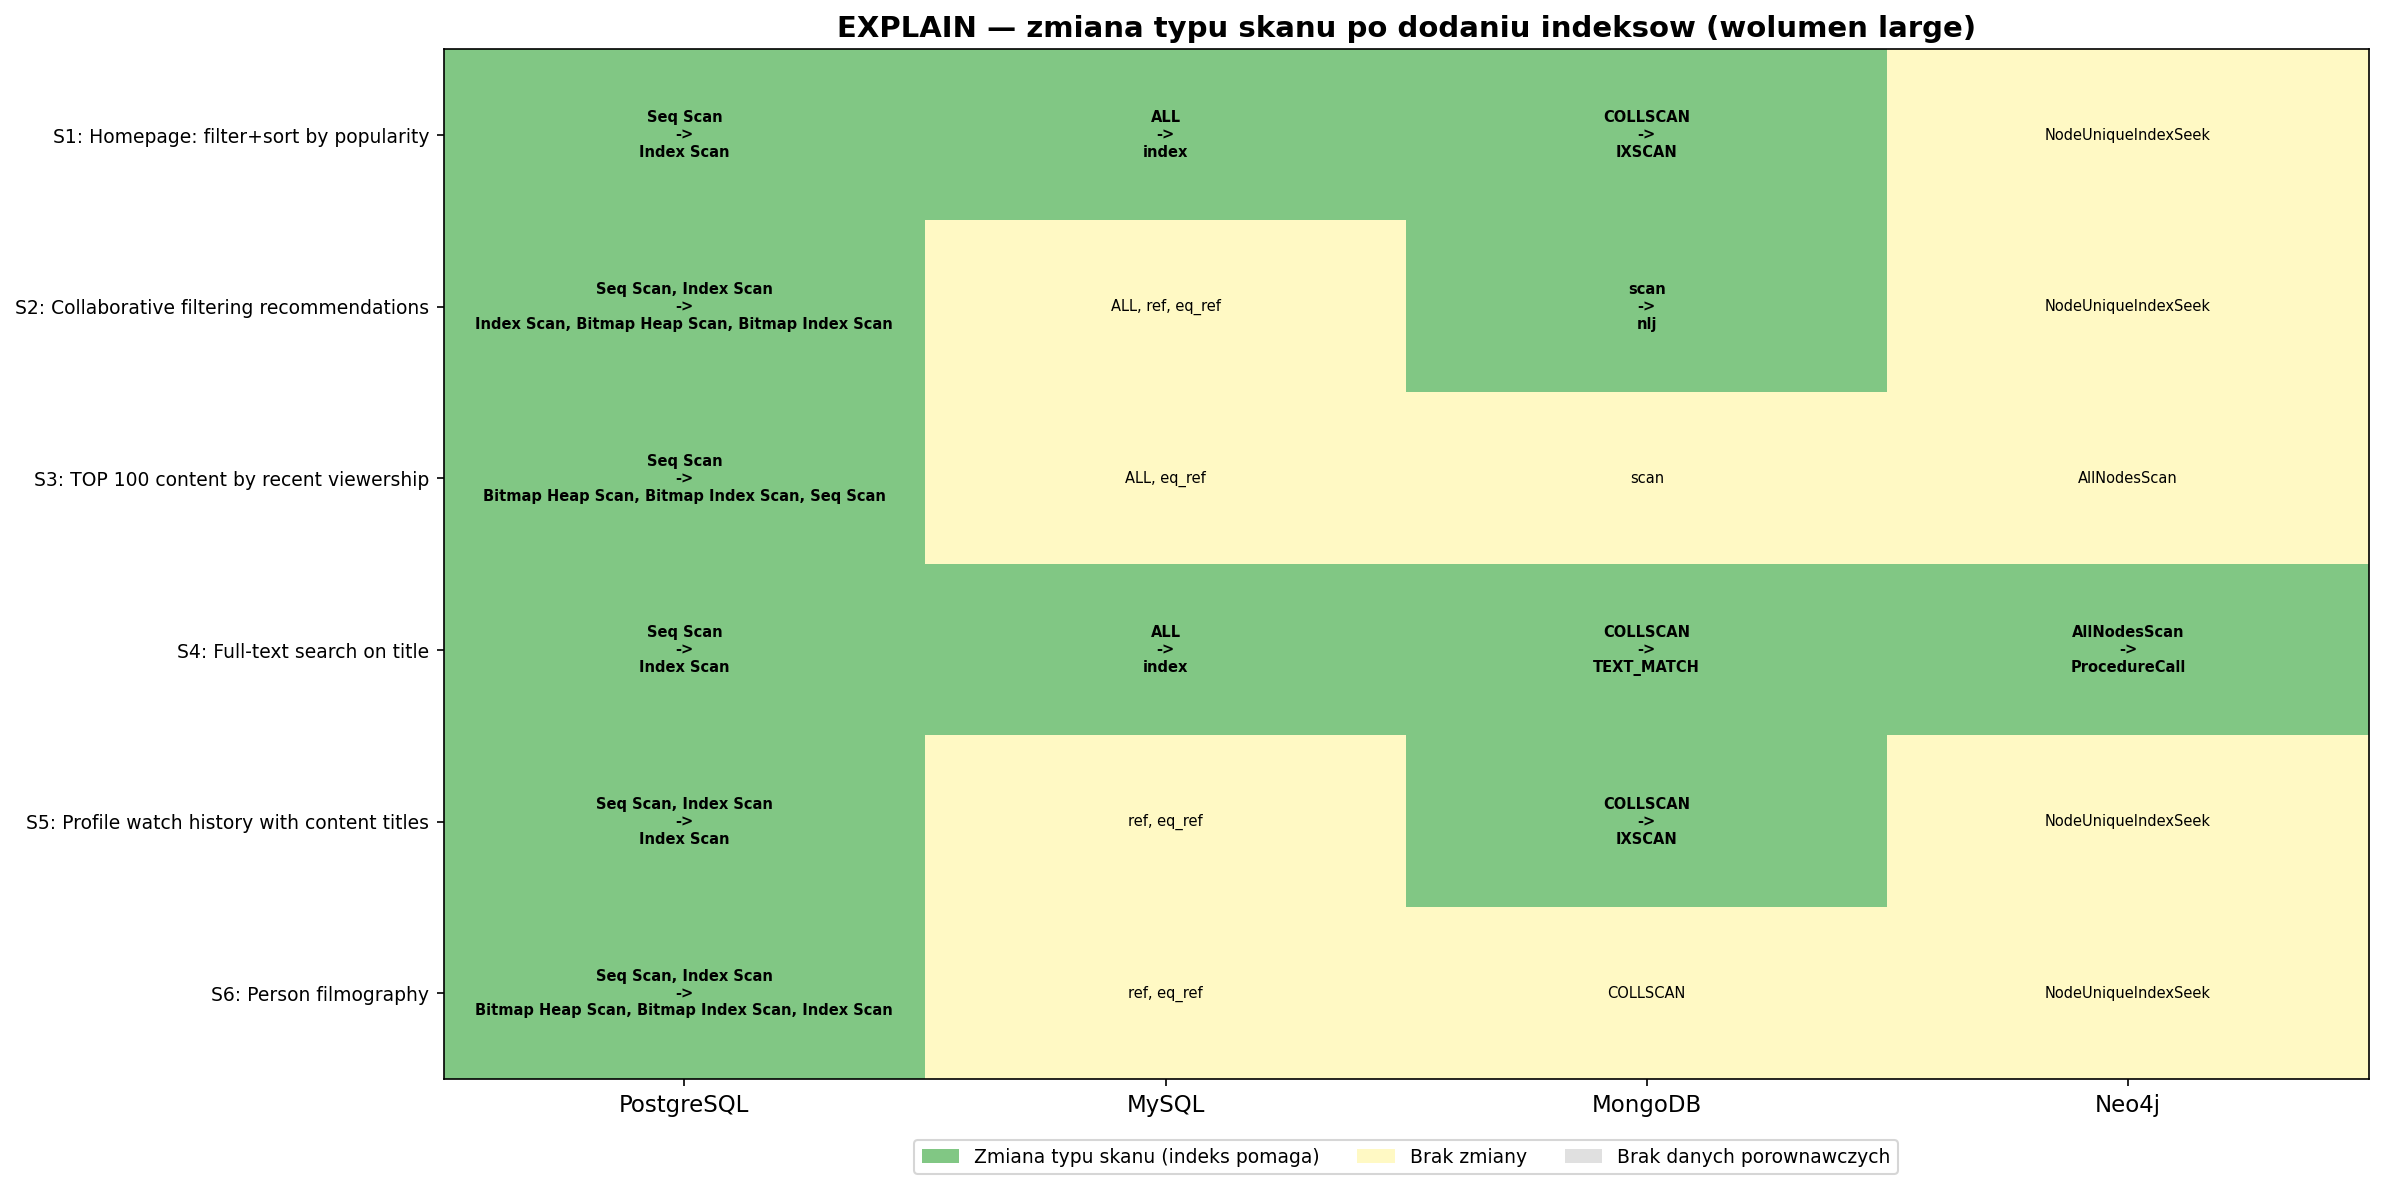
\includegraphics[width=1.0\textwidth]{charts/explain/explain_scan_changes_large.png}
    \caption{Zmiany typów skanów -- wolumen large, bez indeksów}
\end{figure}

\begin{figure}[H]
    \centering
    
\includegraphics[width=1.0\textwidth]{charts/explain/explain_rows_examined_small.png}
    \caption{Liczba przejrzanych wierszy -- wolumen small, bez indeksów}
\end{figure}

\begin{figure}[H]
    \centering
    
\includegraphics[width=1.0\textwidth]{charts/explain/explain_rows_examined_medium.png}
    \caption{Liczba przejrzanych wierszy -- wolumen medium, bez indeksów}
\end{figure}

\begin{figure}[H]
    \centering
    
\includegraphics[width=1.0\textwidth]{charts/explain/explain_rows_examined_large.png}
    \caption{Liczba przejrzanych wierszy -- wolumen large, bez indeksów}
\end{figure}

% -------------------------------------------------------

\subsection{Wyniki z indeksami}

\begin{figure}[H]
    \centering
    
\includegraphics[width=1.0\textwidth]{charts/explain/explain_scan_changes_small.png}
    \caption{Zmiany typów skanów -- wolumen small, z indeksami}
\end{figure}

\begin{figure}[H]
    \centering
    
\includegraphics[width=1.0\textwidth]{charts/explain/explain_scan_changes_medium.png}
    \caption{Zmiany typów skanów -- wolumen medium, z indeksami}
\end{figure}

\begin{figure}[H]
    \centering
    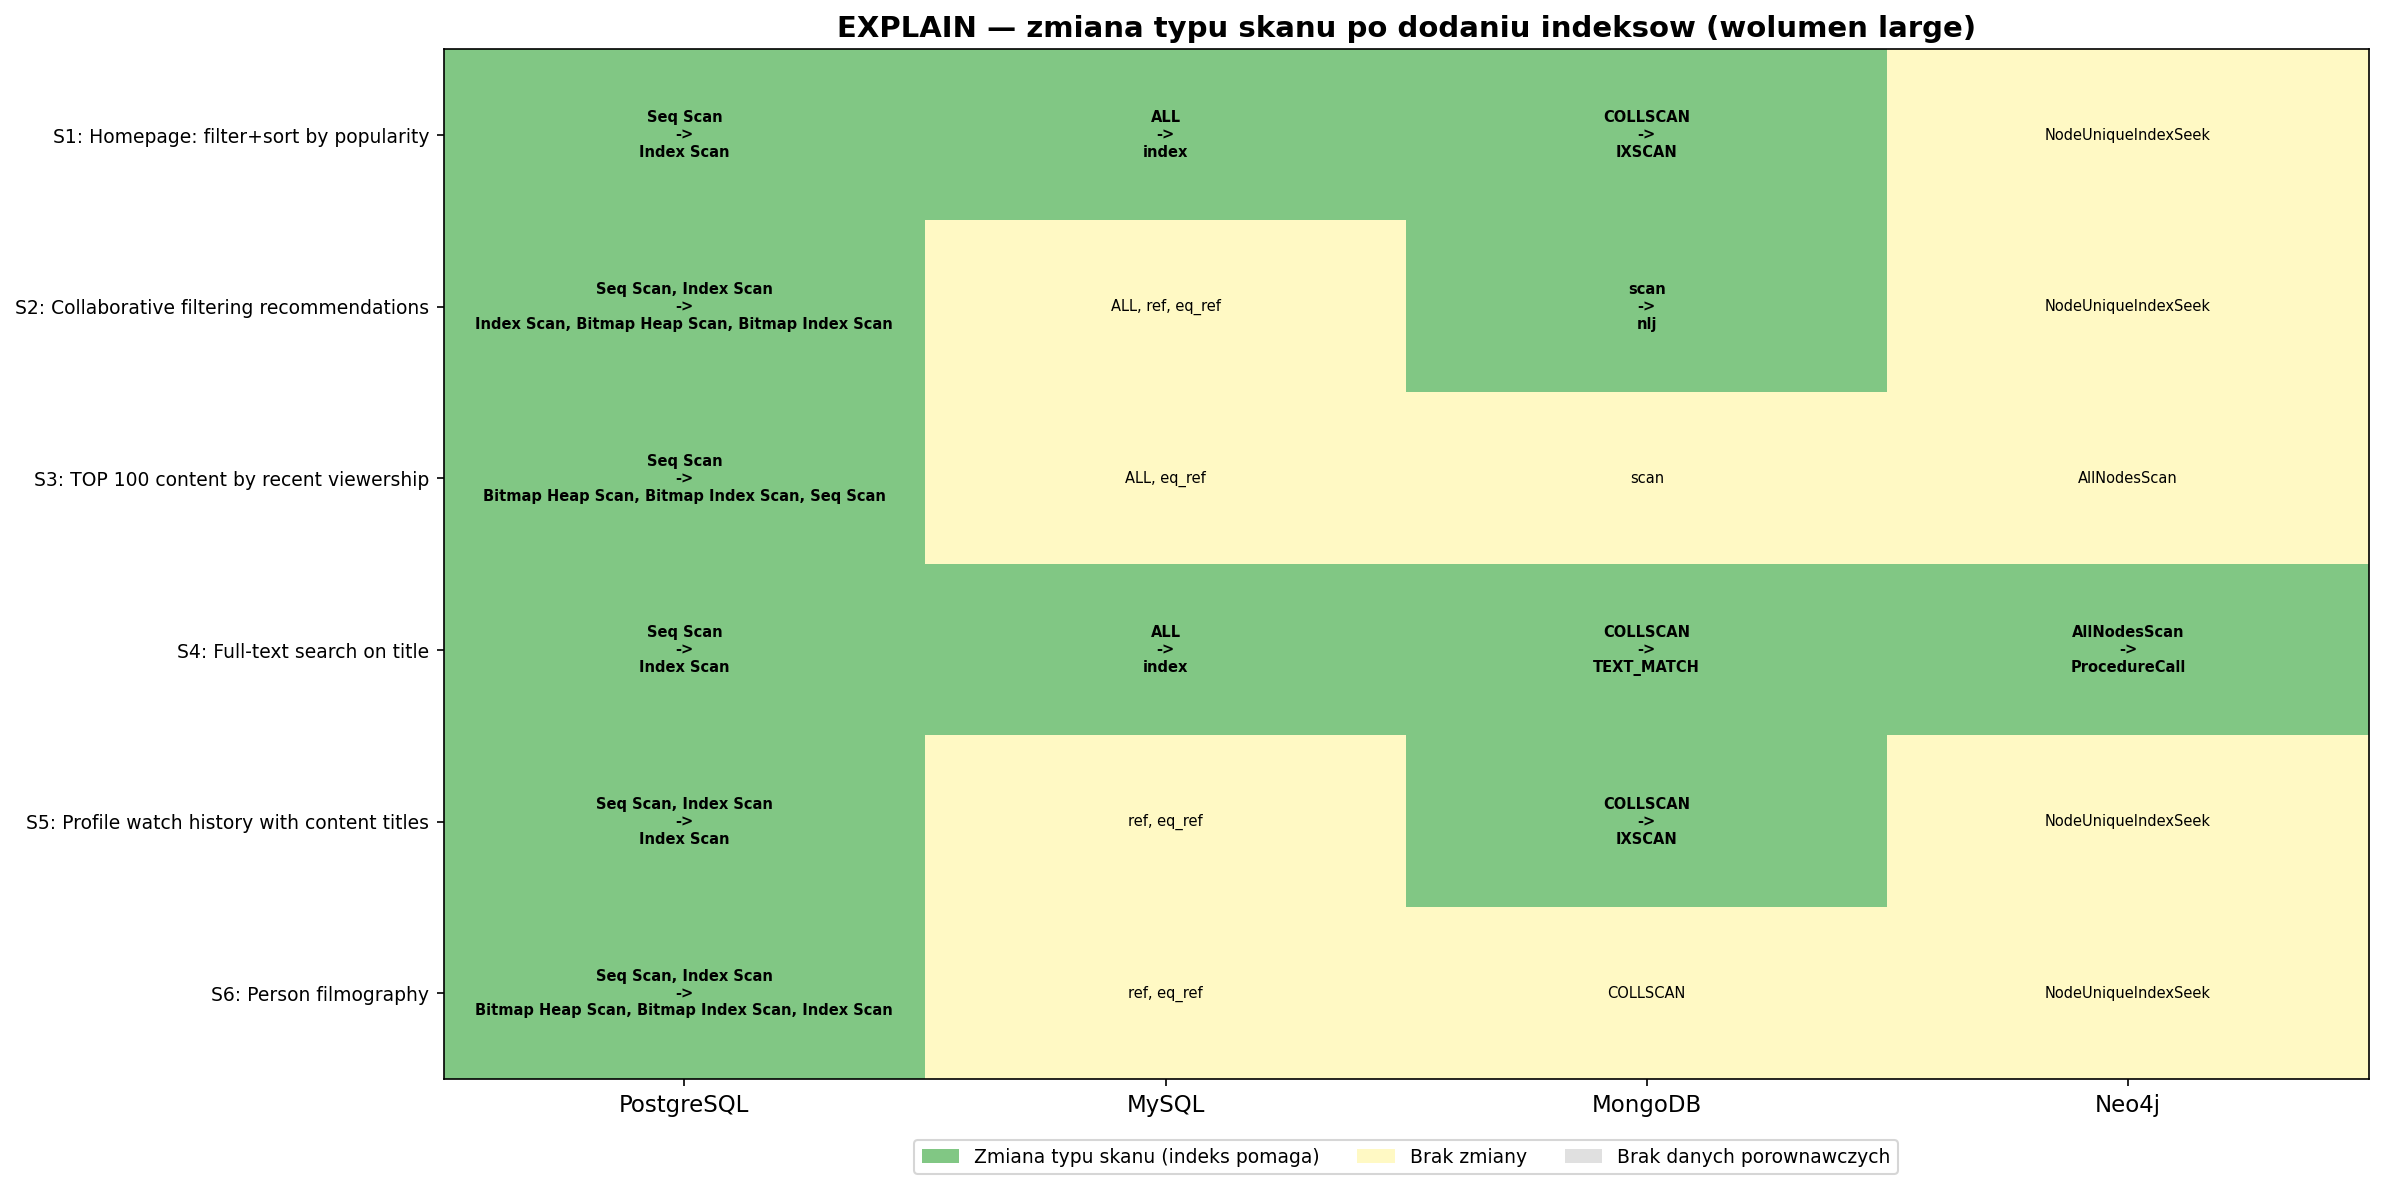
\includegraphics[width=1.0\textwidth]{charts/explain/explain_scan_changes_large.png}
    \caption{Zmiany typów skanów -- wolumen large, z indeksami}
\end{figure}

\begin{figure}[H]
    \centering
    
\includegraphics[width=1.0\textwidth]{charts/explain/explain_rows_examined_small.png}
    \caption{Liczba przejrzanych wierszy -- wolumen small, z indeksami}
\end{figure}

\begin{figure}[H]
    \centering
    
\includegraphics[width=1.0\textwidth]{charts/explain/explain_rows_examined_medium.png}
    \caption{Liczba przejrzanych wierszy -- wolumen medium, z indeksami}
\end{figure}

\begin{figure}[H]
    \centering
    
\includegraphics[width=1.0\textwidth]{charts/explain/explain_rows_examined_large.png}
    \caption{Liczba przejrzanych wierszy -- wolumen large, z indeksami}
\end{figure}

% -------------------------------------------------------

\subsection{Porównanie i wykresy}

\begin{figure}[H]
    \centering
    
\includegraphics[width=1.0\textwidth]{charts/explain/explain_exec_time_small.png}
    \caption{Czas wykonania zapytań SELECT -- wolumen small}
\end{figure}

\begin{figure}[H]
    \centering
    
\includegraphics[width=1.0\textwidth]{charts/explain/explain_exec_time_medium.png}
    \caption{Czas wykonania zapytań SELECT -- wolumen medium}
\end{figure}

\begin{figure}[H]
    \centering
    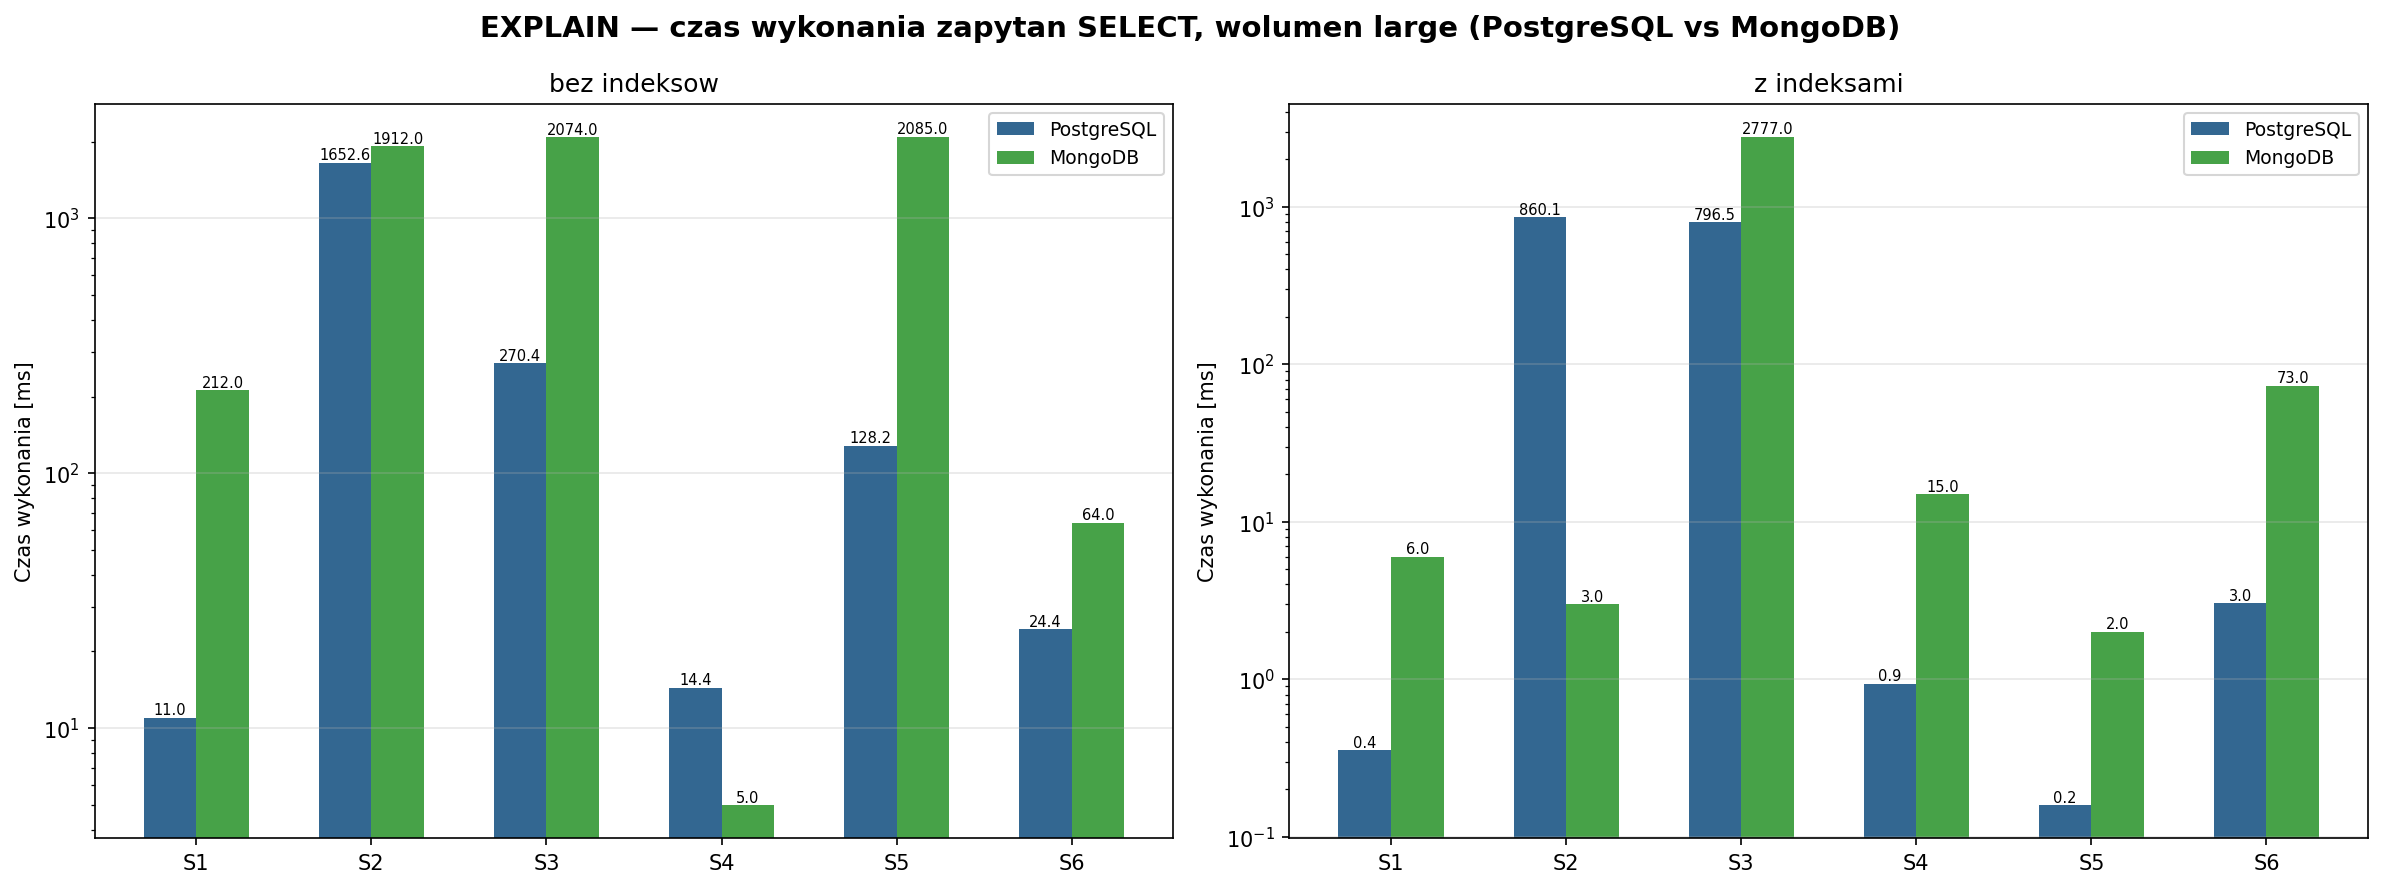
\includegraphics[width=1.0\textwidth]{charts/explain/explain_exec_time_large.png}
    \caption{Czas wykonania zapytań SELECT -- wolumen large}
\end{figure}


% -------------------------------------------------------
\section{Testy wydajnościowe}
\subsection{Wolumen small - 500 000 rekordów}

% -------------------------------------------------------
% INSERT
% -------------------------------------------------------

\subsubsection{I2: Bulk import ocen}
\begin{figure}[H]
    \centering
    
\includegraphics[width=0.8\textwidth]{charts/small/chart_I2.png}
    \caption{I2 -- Bulk import ocen}
\end{figure}

MongoDB jest tu wyraźnie najszybszy (36~ms vs 190--290~ms w pozostałych
silnikach) -- wstawianie dokumentów do kolekcji bez walidacji schematu
jest tańsze niż klasyczny \texttt{INSERT} z kontrolą kluczy obcych
i typów. Założenie indeksów spowalnia Mongo \emph{trzykrotnie}
(z 36 do 111~ms), ponieważ każdy wstawiany dokument musi
zaktualizować strukturę indeksu -- co dobrze potwierdza drugą część
hipotezy pracy. PostgreSQL i MySQL prawie nie odczuwają tej różnicy
między wariantami, bo ich nadrzędna prędkość \texttt{INSERT}-a
i tak jest ograniczona przez WAL/redo log, a nie przez liczbę
indeksów dodatkowych.

\subsubsection{I3: Dodanie serialu z pełnym drzewem}
\begin{figure}[H]
    \centering
    
\includegraphics[width=0.8\textwidth]{charts/small/chart_I3.png}
    \caption{I3 -- Dodanie serialu z pełnym drzewem}
\end{figure}

Tu MongoDB \emph{miażdży} konkurencję -- 0.9~ms wobec 17--25~ms
w pozostałych bazach. Powód jest prosty: w modelu dokumentowym serial
z sezonami i odcinkami to \emph{jeden} dokument zapisywany jednym
wywołaniem \texttt{insert\_one}. W bazach relacyjnych ten sam serial
wymaga osobnych \texttt{INSERT}-ów do tabel \texttt{content},
\texttt{seasons} i \texttt{episodes}, a w Neo4j -- wielu
\texttt{CREATE} dla węzłów i relacji. Indeksy nie wpływają tu
istotnie -- wszystkie operacje są \texttt{INSERT}-ami pojedynczych
encji rzędu kilkunastu rekordów, a koszt zapisu indeksu na takiej
wielkości jest w granicach szumu pomiarowego.

% -------------------------------------------------------
% SELECT
% -------------------------------------------------------

\subsubsection{S2: Filtrowanie kolaboratywne}
\begin{figure}[H]
    \centering
    
\includegraphics[width=0.8\textwidth]{charts/small/chart_S2.png}
    \caption{S2 -- Filtrowanie kolaboratywne}
\end{figure}

MySQL wygrywa we wszystkich wariantach -- dzięki temu, że indeks na
\texttt{profile\_id} jest niemożliwy do upuszczenia (chroni FK -- patrz
uwaga w 11.1), MySQL i tak korzysta z optymalnego planu nawet w
wariancie ,,bez indeksów''. Najmocniejszy zysk daje MongoDB,
który spada ze 158~ms do 16~ms -- to potwierdza obserwację z 11.3,
że bez indeksu na \texttt{profile\_id} Mongo musi skanować całą
kolekcję \texttt{watch\_history}. PostgreSQL halnie czas (z 78 do
40~ms), ale dalej zostaje mu rezydualny \texttt{Seq Scan} z
podzapytania \texttt{NOT IN}. Neo4j najmniej zyskuje, bo i tak
operuje na strukturze grafu, w której indeksy na atrybutach mają
mniejsze znaczenie niż przejścia po krawędziach.

\subsubsection{S3: TOP 100 według liczby ocen w okresie}
\begin{figure}[H]
    \centering
    
\includegraphics[width=0.8\textwidth]{charts/small/chart_S3.png}
    \caption{S3 -- TOP 100 według liczby ocen w okresie}
\end{figure}

PostgreSQL prowadzi (14--16~ms), za nim MongoDB (26--28~ms),
a najwolniejsze są MySQL i Neo4j (38--71~ms). Kluczowa obserwacja:
\textbf{indeks praktycznie nie pomaga} -- w żadnym z silników nie ma
zauważalnej różnicy między wariantami, w MySQL i PostgreSQL nawet
występuje minimalne pogorszenie. Zgadza się to z analizą EXPLAIN
z 11.3: filtr po dacie zwraca tak szeroki zbiór wierszy, że indeks
na \texttt{started\_at} nie zmienia faktu, że trzeba przeczytać
większość tabeli. Ten scenariusz pokazuje granicę użyteczności
indeksu -- dla zapytań z niską selektywnością strukturalna optymalizacja
zapytania (np. agregacje) jest istotniejsza niż obecność indeksu.

\subsubsection{S4: Wyszukiwanie pełnotekstowe po tytule}
\begin{figure}[H]
    \centering
    
\includegraphics[width=0.8\textwidth]{charts/small/chart_S4.png}
    \caption{S4 -- Wyszukiwanie pełnotekstowe po tytule}
\end{figure}

Na małym wolumenie wszystkie cztery silniki radzą sobie szybko
(1.4--7~ms), więc różnice między wariantami są mało spektakularne.
Najwolniejsze jest Neo4j (6.7~ms) -- skan wszystkich węzłów
\texttt{:Content} jest w tej skali odczuwalny. PostgreSQL i MySQL
bez indeksu kończą w niespełna 2~ms, bo w tabeli jest tylko
2\,000 tytułów do przeszukania. Prawdziwa wartość indeksów
pełnotekstowych ujawni się dopiero na wolumenach \emph{medium}
i \emph{large}, gdzie różnica między skanem pełnym a indeksem
sięga rzędów wielkości.

% -------------------------------------------------------
% DELETE
% -------------------------------------------------------

\subsubsection{D1: Usunięcie treści z kaskadą}
\begin{figure}[H]
    \centering
    
\includegraphics[width=0.8\textwidth]{charts/small/chart_D1.png}
    \caption{D1 -- Usunięcie treści z kaskadą}
\end{figure}

PostgreSQL pokazuje tu drugą połowę hipotezy w dobrym świetle:
bez indeksów 17~ms, z indeksami \emph{1.2~ms} -- przyspieszenie
o rząd wielkości. Powodem jest to, że kaskadowe usunięcie
(\texttt{ON DELETE CASCADE}) wymaga znalezienia wszystkich wierszy
potomnych po kluczu obcym -- bez indeksu na FK to oznacza pełen
skan tabel \texttt{watch\_history}, \texttt{ratings} i \texttt{my\_list}.
MongoDB jest tu najwolniejszy w obu wariantach (91~ms / 22~ms),
ponieważ usunięcie treści wymaga skasowania wszystkich powiązanych
dokumentów w innych kolekcjach. MySQL ma stały czas 6~ms, bo indeks
na FK jest u niego zawsze obecny. Neo4j 11--12~ms -- relacje wskazują
na właściwe węzły, więc kaskada to po prostu usunięcie tych krawędzi.

\subsubsection{D4: Usunięcie pozycji z listy}
\begin{figure}[H]
    \centering
    
\includegraphics[width=0.8\textwidth]{charts/small/chart_D4.png}
    \caption{D4 -- Usunięcie pozycji z listy}
\end{figure}

Najprostsza operacja w zestawie -- usunięcie jednego wiersza po
kluczu głównym. PostgreSQL kończy w 1~ms w obu wariantach,
MongoDB z indeksem zjeżdża do 0.6~ms. Bez indeksu MongoDB potrzebuje
20~ms -- klasyczny przypadek, w którym \texttt{deleteOne} bez
indeksu i tak musi przeskanować kolekcję, żeby znaleźć dokument
do usunięcia. To samo zjawisko będzie się skalować liniowo
z wolumenem (zobaczymy 200~ms na \emph{large}). MySQL i Neo4j
działają stabilnie 5--8~ms.

\subsubsection{D6: Masowe usunięcie nieaktywnych użytkowników}
\begin{figure}[H]
    \centering
    
\includegraphics[width=0.8\textwidth]{charts/small/chart_D6.png}
    \caption{D6 -- Masowe usunięcie nieaktywnych użytkowników}
\end{figure}

Pierwszy scenariusz, w którym brak indeksu boli naprawdę mocno --
PostgreSQL bez indeksu na \texttt{users.status} kończy w 37~ms,
a z indeksem w 1.2~ms (30-krotnie szybciej). To kluczowy wynik
wspierający hipotezę: indeks dramatycznie przyspiesza znajdowanie
podzbioru wierszy do usunięcia, bo zamiast pełnego skanu \texttt{users}
silnik trafia od razu na rekordy ze statusem ,,inactive''. MongoDB
i Neo4j również zyskują (0.8 i 7~ms odpowiednio), ale dystans nie
jest tak spektakularny. \emph{Spektakularne} skutki braku indeksu
zobaczymy dopiero na większych wolumenach -- na \emph{large}
PostgreSQL bez indeksu osiągnie pomiar mierzony w \emph{sekundach}.

% -------------------------------------------------------
% UPDATE
% -------------------------------------------------------

\subsubsection{U2: Przeliczenie średniej oceny}
\begin{figure}[H]
    \centering
    
\includegraphics[width=0.8\textwidth]{charts/small/chart_U2.png}
    \caption{U2 -- Przeliczenie średniej oceny}
\end{figure}

PostgreSQL z indeksem schodzi z 3.7~ms do 1.3~ms, MongoDB z 11~ms
do 1.7~ms. Operacja przelicza średnią ocenę wybranego filmu
i wykonuje \texttt{UPDATE} pojedynczego wiersza/dokumentu --
indeks pomaga zlokalizować zarówno źródłowe oceny (\texttt{ratings})
jak i wiersz w \texttt{content}. MySQL ma stały czas 6~ms, Neo4j
4--6~ms. To typowy operacyjny scenariusz, w którym indeks działa
zgodnie z oczekiwaniami -- punktowy filtr + pojedyncza modyfikacja
to klasyczny ,,słodki punkt'' indeksu dodatkowego, czyli wąski filtr
\texttt{WHERE} bez konfliktu z dużymi zapisami.

\subsubsection{U3: Masowa zmiana planu subskrypcji}
\begin{figure}[H]
    \centering
    
\includegraphics[width=0.8\textwidth]{charts/small/chart_U3.png}
    \caption{U3 -- Masowa zmiana planu subskrypcji}
\end{figure}

Najciekawszy wynik tej kategorii i \emph{dowód kosztu indeksów dla
operacji zapisu}. PostgreSQL bez indeksu kończy w 8.9~ms, z indeksem
w \emph{16.9~ms} -- czyli założenie indeksów pogorszyło wydajność
prawie dwukrotnie. To samo widać w MySQL (38 → 52~ms), Mongo
(29 → 33~ms) i Neo4j (53 → 43~ms tylko z lekkim odchyleniem).
Operacja modyfikuje pole \texttt{plan\_name} w wielu wierszach
\texttt{subscriptions} -- każdy zaktualizowany wiersz wymaga
przepisania w indeksie \texttt{idx\_subscriptions\_status\_plan},
co dodaje stały narzut do każdej zmiany. Ten scenariusz najwyraźniej
ze wszystkich potwierdza drugą część hipotezy: indeksy podnoszą
koszt operacji \texttt{UPDATE} na kolumnach indeksowanych.


\subsection{Wolumen medium - 1 000 000 rekordów}

% -------------------------------------------------------
% INSERT
% -------------------------------------------------------

\subsubsection{I2: Bulk import ocen}
\begin{figure}[H]
    \centering
    
\includegraphics[width=0.8\textwidth]{charts/medium/chart_I2.png}
    \caption{I2 -- Bulk import ocen}
\end{figure}

Wzrost wolumenu ujawnia, jak bardzo \texttt{INSERT} jest operacją
liniową w liczbie wstawianych wierszy. PostgreSQL i MySQL skaczą
z 270/190~ms na 1.2/1.4~s -- niemal pięciokrotnie. MongoDB zachowuje
przewagę (461~ms vs 1.2--3.5~s u konkurencji), ale traci ją po
założeniu indeksów (1.1~s -- prawie tyle co PostgreSQL). Neo4j
płaci najwyższą cenę -- 3.5~s niezależnie od indeksów -- co wynika
z konieczności tworzenia osobnych węzłów \texttt{:Rating} dla każdej
oceny i wiązania ich relacjami do \texttt{:Profile} i \texttt{:Content}.

\subsubsection{I3: Dodanie serialu z pełnym drzewem}
\begin{figure}[H]
    \centering
    
\includegraphics[width=0.8\textwidth]{charts/medium/chart_I3.png}
    \caption{I3 -- Dodanie serialu z pełnym drzewem}
\end{figure}

Rozkład sił identyczny jak na \emph{small} -- dowód, że ten scenariusz
jest praktycznie \emph{niezależny od wolumenu danych} (wstawiamy
zawsze ten sam ,,jeden serial''). MongoDB \emph{0.7~ms}, pozostali
15--30~ms. Niezmienność wyniku potwierdza, że koszt \texttt{INSERT}-a
pojedynczej encji nie zależy od rozmiaru tabeli docelowej -- liczy
się tylko narzut samej operacji zapisu i utrzymania indeksów na tym
konkretnym wierszu.

% -------------------------------------------------------
% SELECT
% -------------------------------------------------------

\subsubsection{S2: Filtrowanie kolaboratywne}
\begin{figure}[H]
    \centering
    
\includegraphics[width=0.8\textwidth]{charts/medium/chart_S2.png}
    \caption{S2 -- Filtrowanie kolaboratywne}
\end{figure}

Indeksy zaczynają działać spektakularnie. Z indeksami \emph{wszystkie}
silniki schodzą do 1.6--5.5~ms -- a bez nich PostgreSQL i MongoDB
mierzą się z 40--97~ms. To pierwszy moment, w którym hipoteza pracy
ma jednoznacznie potwierdzającą postać: indeks redukuje czas SELECT-a
o \emph{rząd wielkości lub więcej}. Neo4j najszybszy bez indeksów
(8~ms) -- struktura grafu zaczyna się tu opłacać.

\subsubsection{S3: TOP 100 według liczby ocen w okresie}
\begin{figure}[H]
    \centering
    
\includegraphics[width=0.8\textwidth]{charts/medium/chart_S3.png}
    \caption{S3 -- TOP 100 według liczby ocen w okresie}
\end{figure}

Trend ze \emph{small} się utrzymuje -- indeks niewiele pomaga, bo
filtr ,,od czerwca'' pokrywa za szeroki podzbiór. PostgreSQL nadal
najszybszy (15--18~ms), Neo4j skacze do 100~ms ze względu na koszt
przechodzenia po wszystkich krawędziach \texttt{:WATCHED}.
MySQL stabilnie 60~ms. Brak istotnej różnicy między wariantami
indeksowymi w żadnym z silników.

\subsubsection{S4: Wyszukiwanie pełnotekstowe po tytule}
\begin{figure}[H]
    \centering
    
\includegraphics[width=0.8\textwidth]{charts/medium/chart_S4.png}
    \caption{S4 -- Wyszukiwanie pełnotekstowe po tytule}
\end{figure}

Tu dopiero widać prawdziwą wartość indeksu pełnotekstowego.
Bez indeksów Neo4j wykonuje \texttt{AllNodesScan} na 5\,000 węzłach --
30~ms. Z indeksem (\texttt{db.index.fulltext.queryNodes}) schodzi do
4~ms. PostgreSQL z trygramowym GIN-em: 0.9~ms (poprawa o 4×).
MongoDB z indeksem \texttt{text}: 1.2~ms (poprawa o 4×). MySQL --
jak pokazaliśmy w 11.3 -- nie aktywuje indeksu \texttt{FULLTEXT}
dla operatora \texttt{LIKE '\%term\%'}, więc obie wartości są
porównywalne (2.8 / 1.3~ms).

% -------------------------------------------------------
% DELETE
% -------------------------------------------------------

\subsubsection{D1: Usunięcie treści z kaskadą}
\begin{figure}[H]
    \centering
    
\includegraphics[width=0.8\textwidth]{charts/medium/chart_D1.png}
    \caption{D1 -- Usunięcie treści z kaskadą}
\end{figure}

Skala intensyfikuje obraz znany ze \emph{small}: PostgreSQL bez
indeksu 24~ms, z indeksem 1.3~ms (18-krotne przyspieszenie). MongoDB
bez indeksu 136~ms, z indeksem 57~ms (2.4-krotnie). MySQL i Neo4j
działają stabilnie 6 i 9~ms odpowiednio. Indeksy na FK są tu
\emph{kluczowe} -- bez nich kaskadowe usunięcie staje się sumą
pełnych skanów wszystkich tabel zależnych.

\subsubsection{D4: Usunięcie pozycji z listy}
\begin{figure}[H]
    \centering
    
\includegraphics[width=0.8\textwidth]{charts/medium/chart_D4.png}
    \caption{D4 -- Usunięcie pozycji z listy}
\end{figure}

Trend liniowy MongoDB w wariancie bez indeksu się potwierdza --
20~ms na \emph{small}, 55~ms na \emph{medium}. Z indeksem to wciąż
0.7~ms, czyli \emph{80-krotna} różnica. PostgreSQL i MySQL stabilne
poniżej 6~ms. Ten prosty scenariusz najwyraźniej obrazuje regułę:
\texttt{deleteOne} bez indeksu jest \texttt{COLLSCAN}-em, koniec
historii.

\subsubsection{D6: Masowe usunięcie nieaktywnych użytkowników}
\begin{figure}[H]
    \centering
    
\includegraphics[width=0.8\textwidth]{charts/medium/chart_D6.png}
    \caption{D6 -- Masowe usunięcie nieaktywnych użytkowników}
\end{figure}

Zaczyna być \emph{dramatycznie}. PostgreSQL bez indeksu na
\texttt{users.status} -- \textbf{1.4~sekundy}, z indeksem 3.3~ms.
To 425-krotne przyspieszenie -- jeden z najmocniejszych wyników
w pracy. MongoDB i Neo4j odpowiednio 2/4~ms i 28/10~ms -- też
zyskują, ale bez tej dramaturgii. MySQL stabilnie 8~ms. Na
\emph{large} ten kontrast pokaże się jeszcze mocniej -- PostgreSQL
przekroczy 30~sekund.

% -------------------------------------------------------
% UPDATE
% -------------------------------------------------------

\subsubsection{U2: Przeliczenie średniej oceny}
\begin{figure}[H]
    \centering
    
\includegraphics[width=0.8\textwidth]{charts/medium/chart_U2.png}
    \caption{U2 -- Przeliczenie średniej oceny}
\end{figure}

PostgreSQL: 8.8 → 1.5~ms (5×). MongoDB: 30 → 1.6~ms (19×). MySQL
stabilnie 6~ms, Neo4j 4~ms. Pojedynczy \texttt{UPDATE} po znalezieniu
wiersza z agregatu, wzorzec znany z \emph{small} -- tylko skala
narzutu wzrasta tam, gdzie indeksu brakuje. Indeks robi tu robotę
oczekiwaną (przyspiesza punktowy filtr), bez negatywnego wpływu
na samą operację zapisu, bo modyfikujemy jeden wiersz.

\subsubsection{U3: Masowa zmiana planu subskrypcji}
\begin{figure}[H]
    \centering
    
\includegraphics[width=0.8\textwidth]{charts/medium/chart_U3.png}
    \caption{U3 -- Masowa zmiana planu subskrypcji}
\end{figure}

Koszt utrzymania indeksów przy modyfikacji wierszy zaczyna być
zauważalny. PostgreSQL bez indeksu 30~ms,
z indeksem 65~ms (ponad dwukrotne pogorszenie). MySQL 124 → 179~ms,
Mongo 107 → 104~ms (tu indeks praktycznie neutralny). Neo4j
zachowuje się odwrotnie -- 194 → 158~ms (lekkie polepszenie),
prawdopodobnie dlatego że \texttt{plan\_name} nie jest indeksowany
w grafie. Im więcej zaktualizowanych wierszy i im więcej indeksów
na zmienianej kolumnie, tym wyższa kara czasowa -- to jest
podręcznikowy efekt utrzymania indeksu przy modyfikacji.


\subsection{Wolumen large - 10 000 000 rekordów}

% -------------------------------------------------------
% INSERT
% -------------------------------------------------------

\subsubsection{I2: Bulk import ocen}
\begin{figure}[H]
    \centering
    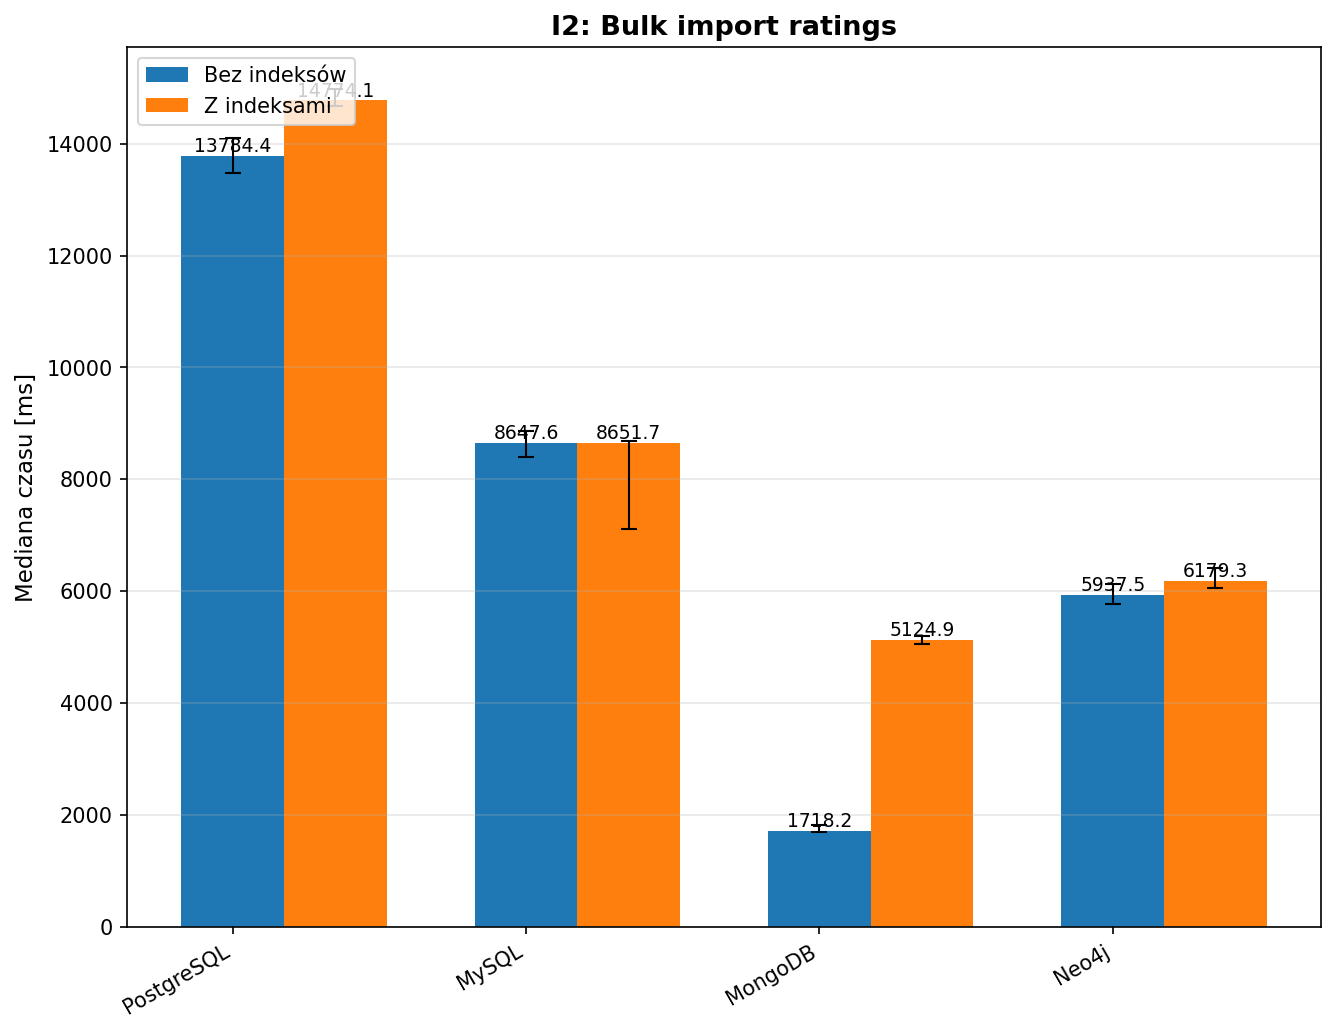
\includegraphics[width=0.8\textwidth]{charts/large/chart_I2.png}
    \caption{I2 -- Bulk import ocen}
\end{figure}

Pełna skala uwidacznia różnice między silnikami w \texttt{INSERT}-ach
masowych. PostgreSQL osiąga \emph{14~sekund} -- to konsekwencja
zarówno utrzymania WAL, jak i indeksów. MySQL 8.6~s, Neo4j 5.9~s
(co ciekawe: na małych wolumenach Neo4j był najwolniejszy, ale tu
jego architektura wsadowego \texttt{UNWIND CREATE} amortyzuje się
lepiej). MongoDB nadal najszybszy bez indeksów (1.7~s), ale z indeksami
zwalnia trzykrotnie do 5.1~s. Indeks dodatkowy daje tu wyraźną karę
czasową we wszystkich silnikach.

\subsubsection{I3: Dodanie serialu z pełnym drzewem}
\begin{figure}[H]
    \centering
    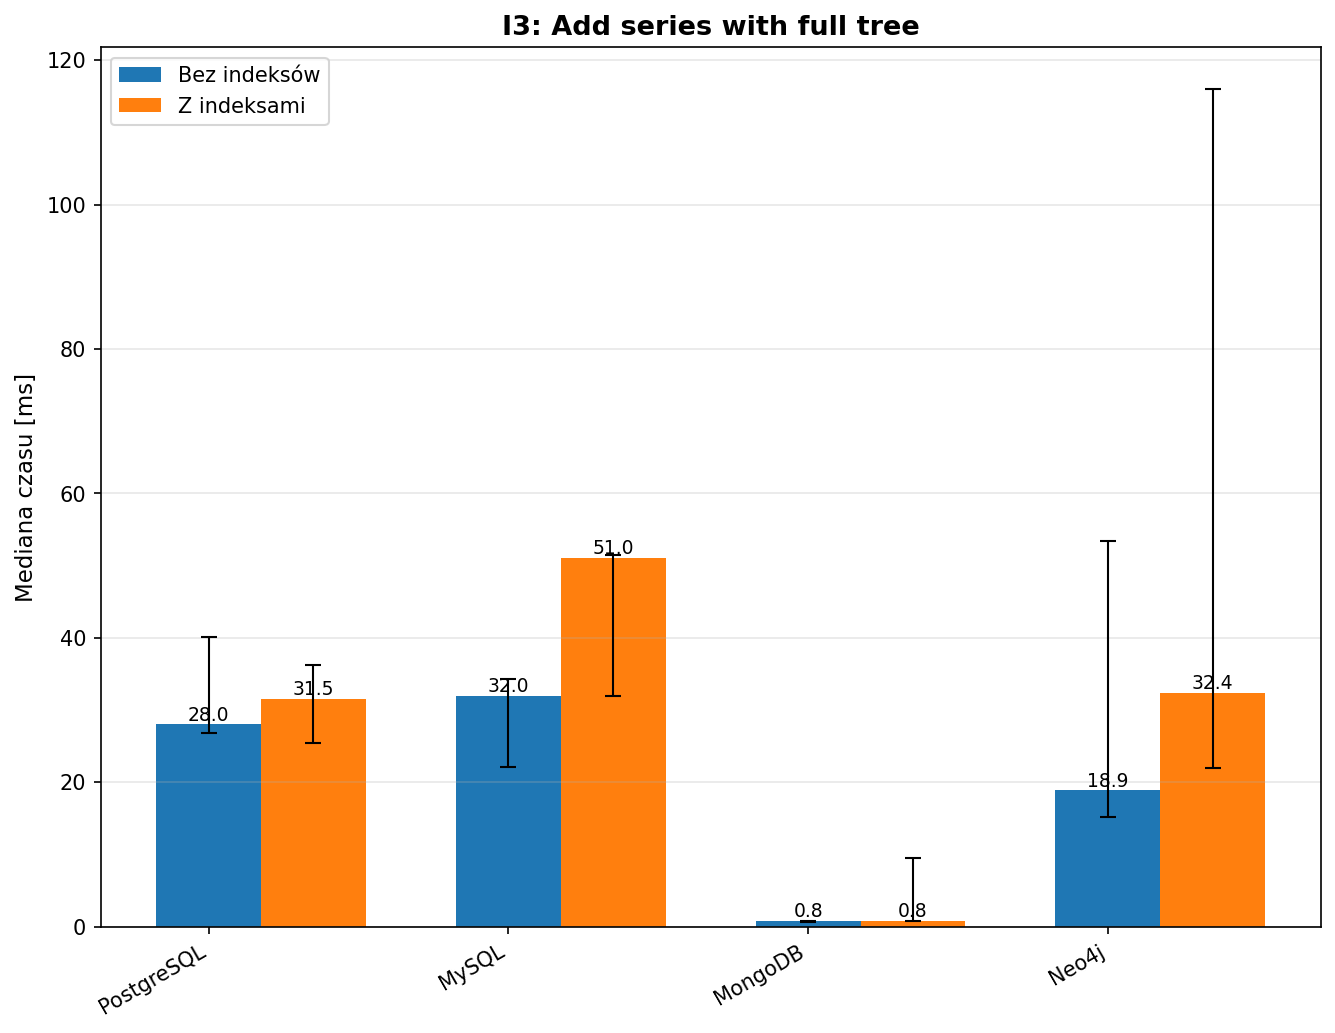
\includegraphics[width=0.8\textwidth]{charts/large/chart_I3.png}
    \caption{I3 -- Dodanie serialu z pełnym drzewem}
\end{figure}

Wynik praktycznie identyczny jak na \emph{small} i \emph{medium} --
MongoDB 0.8~ms, pozostali 18--51~ms. Niezależność od wolumenu
potwierdza się w pełni: koszt pojedynczego \texttt{INSERT}-a serialu
nie rośnie z rozmiarem katalogu, bo nowo wstawiany rekord zostaje
po prostu dopisany na końcu. Większy wolumen spowodował tylko
dwukrotny wzrost czasu w MySQL z indeksami (19 → 51~ms) -- to
narzut przebudowy indeksu \texttt{FULLTEXT} przy każdym dopisanym
rekordzie.

% -------------------------------------------------------
% SELECT
% -------------------------------------------------------

\subsubsection{S2: Filtrowanie kolaboratywne}
\begin{figure}[H]
    \centering
    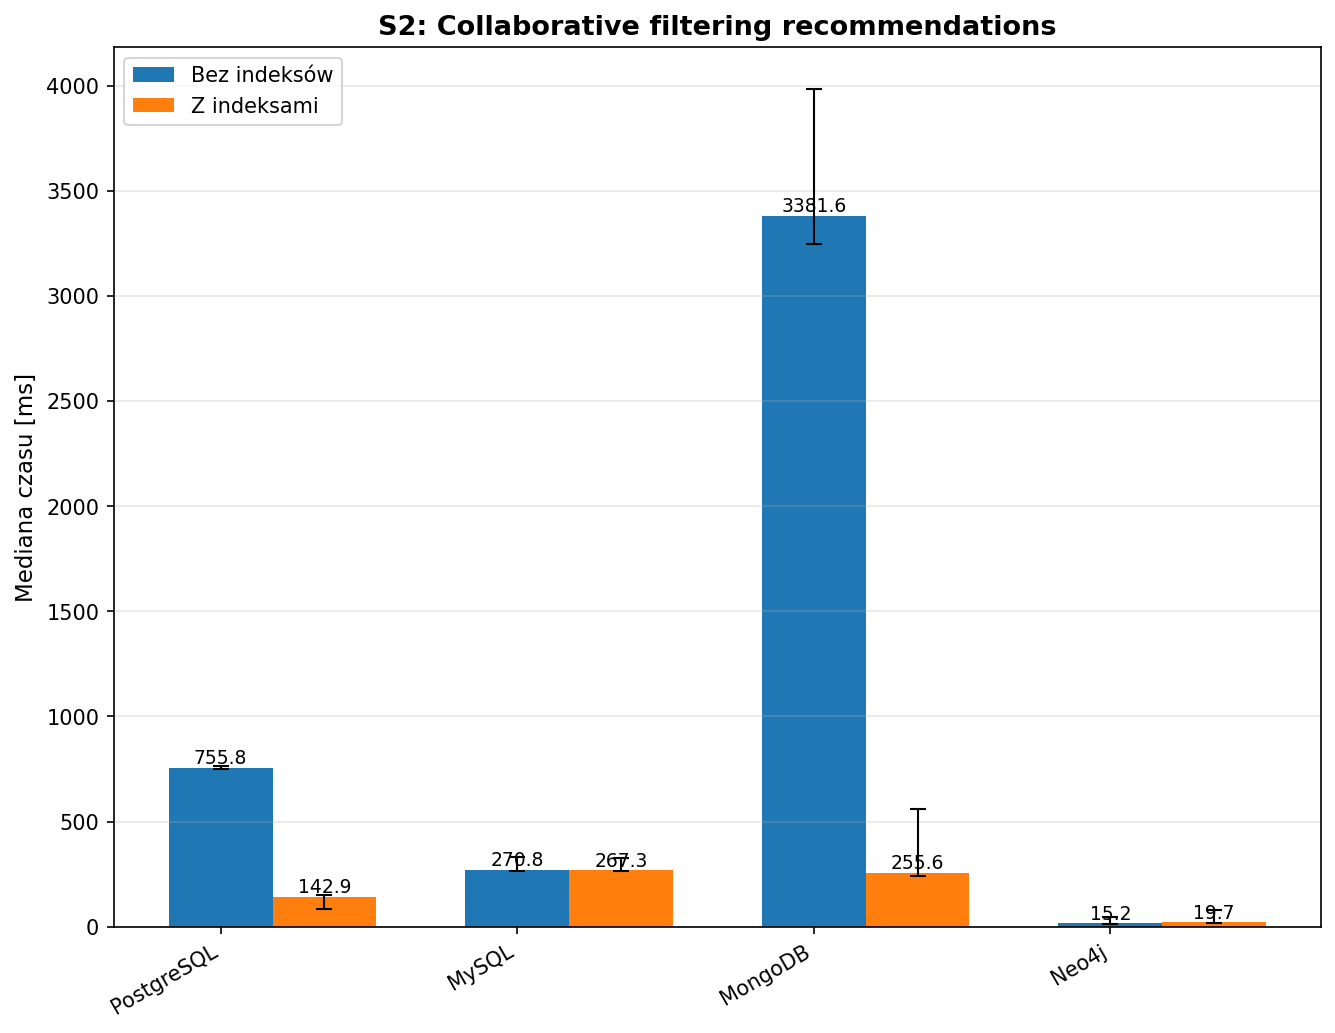
\includegraphics[width=0.8\textwidth]{charts/large/chart_S2.png}
    \caption{S2 -- Filtrowanie kolaboratywne}
\end{figure}

\textbf{Neo4j zostawia konkurencję daleko z tyłu} -- 15~ms bez
indeksów, 19~ms z indeksami. Pozostałe bazy bez indeksów osiągają sekundy:
PostgreSQL 755~ms, MySQL 270~ms, Mongo \emph{3.4~sekundy} (skan
6 milionów dokumentów). Z indeksami PG schodzi do 142~ms, Mongo do
255~ms -- ale Neo4j i tak pozostaje 8--15× szybszy. Ten scenariusz
najlepiej pokazuje, kiedy graf wygrywa: wielokrotne ,,wskakiwanie''
między profilami i treścią to nawigacja po krawędziach, w której
relacja jest fizycznym wskaźnikiem -- zamiast kolejnych \texttt{JOIN}-ów
po milionach wierszy.

\subsubsection{S3: TOP 100 według liczby ocen w okresie}
\begin{figure}[H]
    \centering
    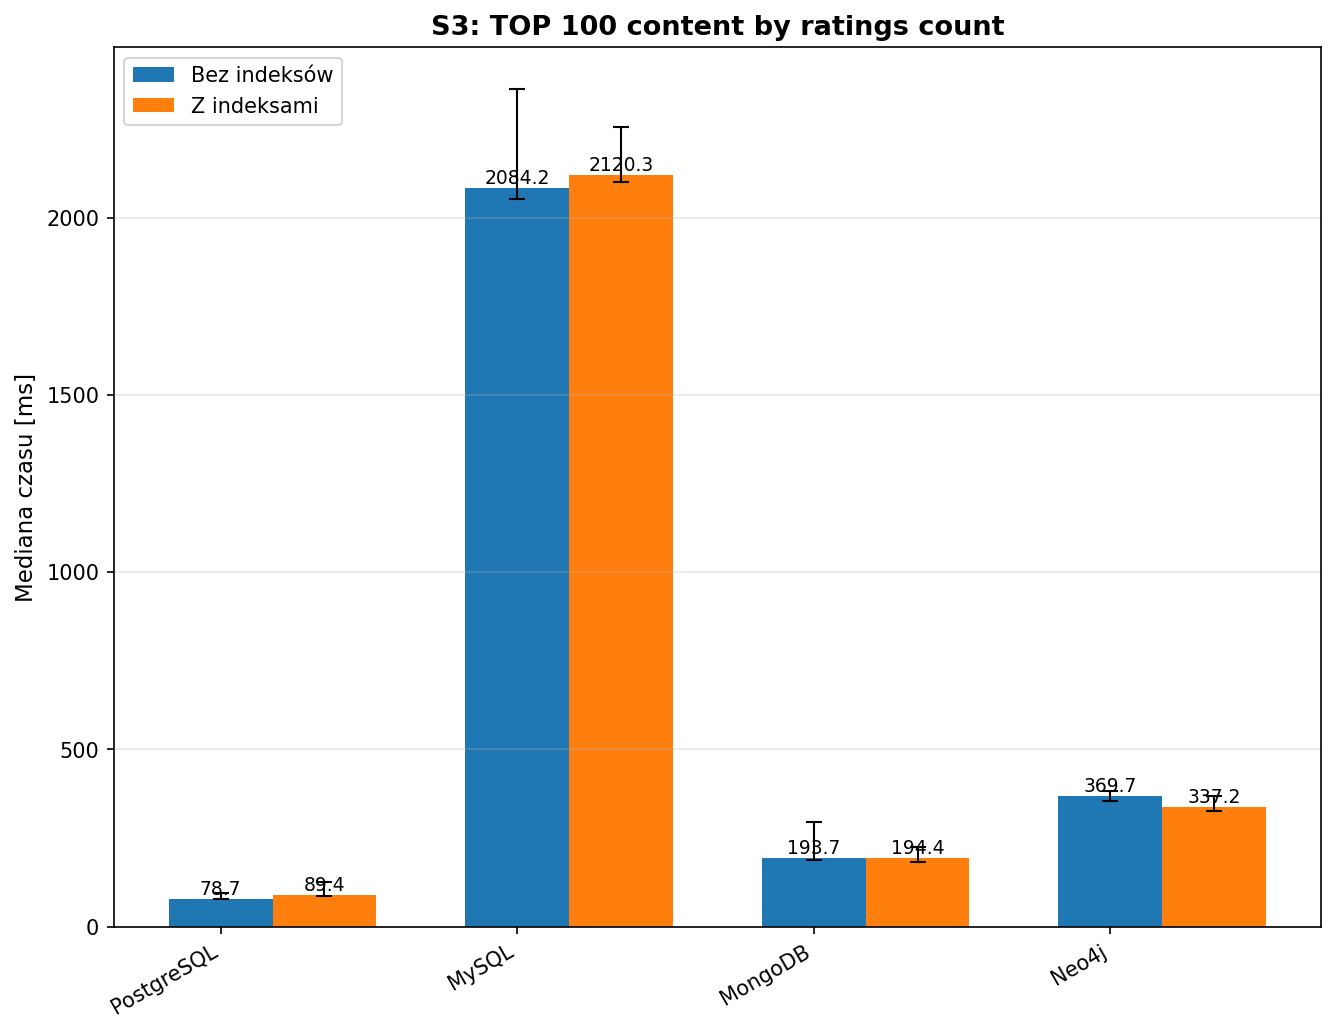
\includegraphics[width=0.8\textwidth]{charts/large/chart_S3.png}
    \caption{S3 -- TOP 100 według liczby ocen w okresie}
\end{figure}

Tu zaczynają się \emph{poważne} różnice. PostgreSQL nadal najszybszy
(79~ms), MySQL 2.1~sekundy(!), MongoDB 194~ms, Neo4j 370~ms. Indeksy
nie pomagają -- wszystkie warianty mają porównywalne czasy do
wariantu bez indeksów. PostgreSQL wygrywa dzięki efektywnemu
wykonaniu agregacji \texttt{COUNT(*)} z grupowaniem; MySQL traci
przez nieefektywny plan z pełnym skanem 5.7~mln wierszy
(potwierdzone w 11.3). To jeden z dwóch scenariuszy w pracy
(obok S2 dla Neo4j), w których architektura silnika znaczy
więcej niż obecność indeksu.

\subsubsection{S4: Wyszukiwanie pełnotekstowe po tytule}
\begin{figure}[H]
    \centering
    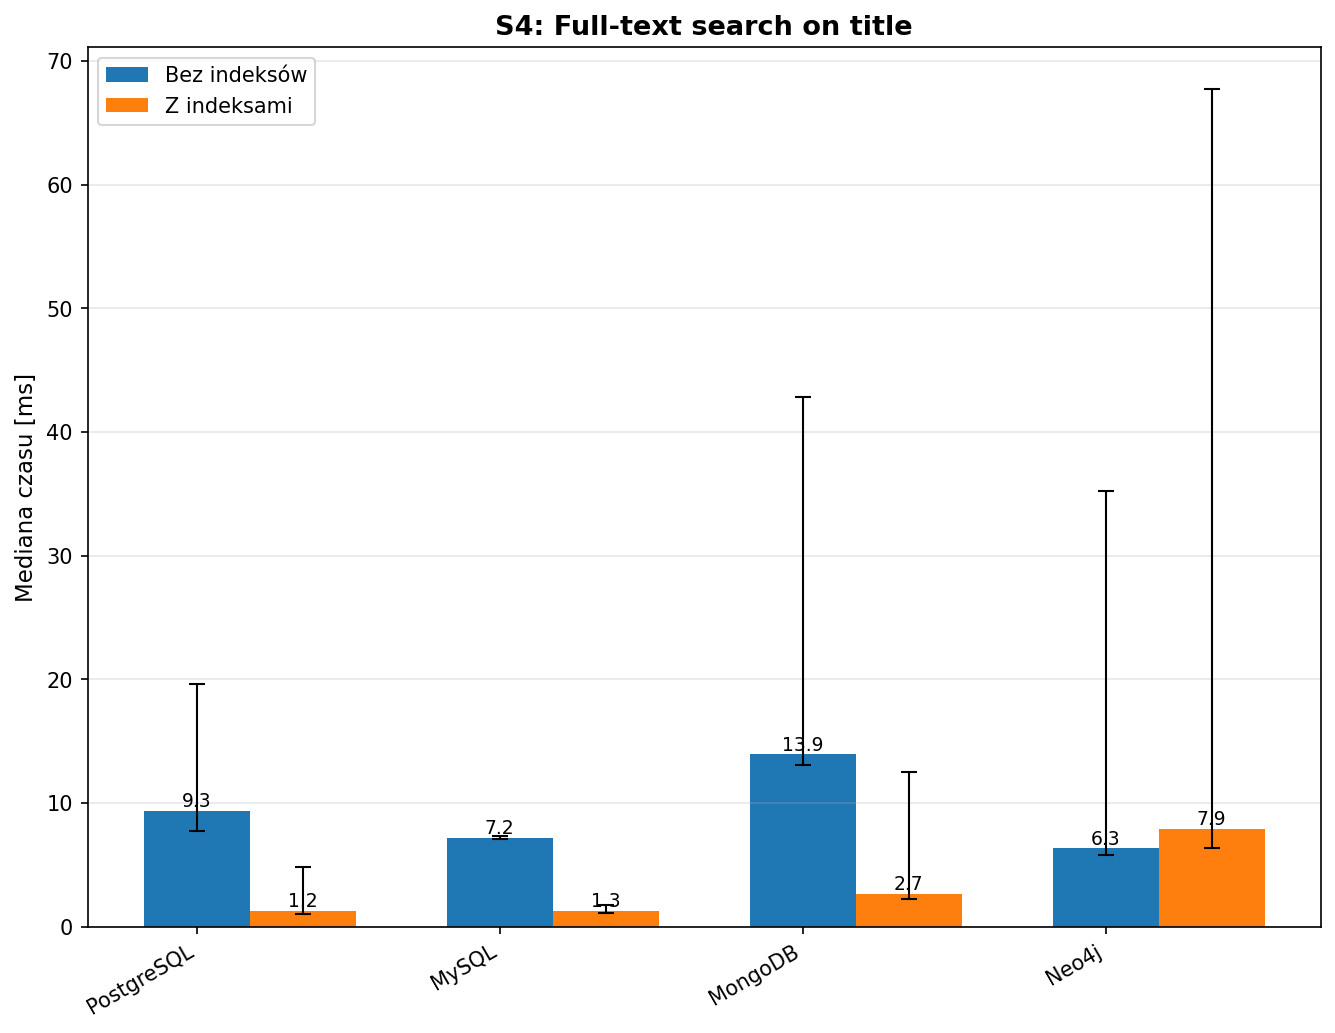
\includegraphics[width=0.8\textwidth]{charts/large/chart_S4.png}
    \caption{S4 -- Wyszukiwanie pełnotekstowe po tytule}
\end{figure}

Indeksy pełnotekstowe działają wzorowo -- bez nich silniki sięgają
7--14~ms (Neo4j najszybszy 6.3~ms dzięki temu, że i tak skanuje
,,tylko'' 15\,000 węzłów), z indeksami wszystkie spadają do
1--3~ms (poza Neo4j -- tam paradoksalnie wzrost do 7.9~ms,
możliwy artefakt cache'u Lucene). PostgreSQL z trygramowym GIN-em
schodzi do 1.2~ms -- ośmiokrotne przyspieszenie. MongoDB z indeksem
\texttt{text}: 2.7~ms (5×). To podręcznikowe potwierdzenie wartości
indeksu pełnotekstowego dla wyszukiwania po wzorcach z wiodącym
,,\%''.

% -------------------------------------------------------
% DELETE
% -------------------------------------------------------

\subsubsection{D1: Usunięcie treści z kaskadą}
\begin{figure}[H]
    \centering
    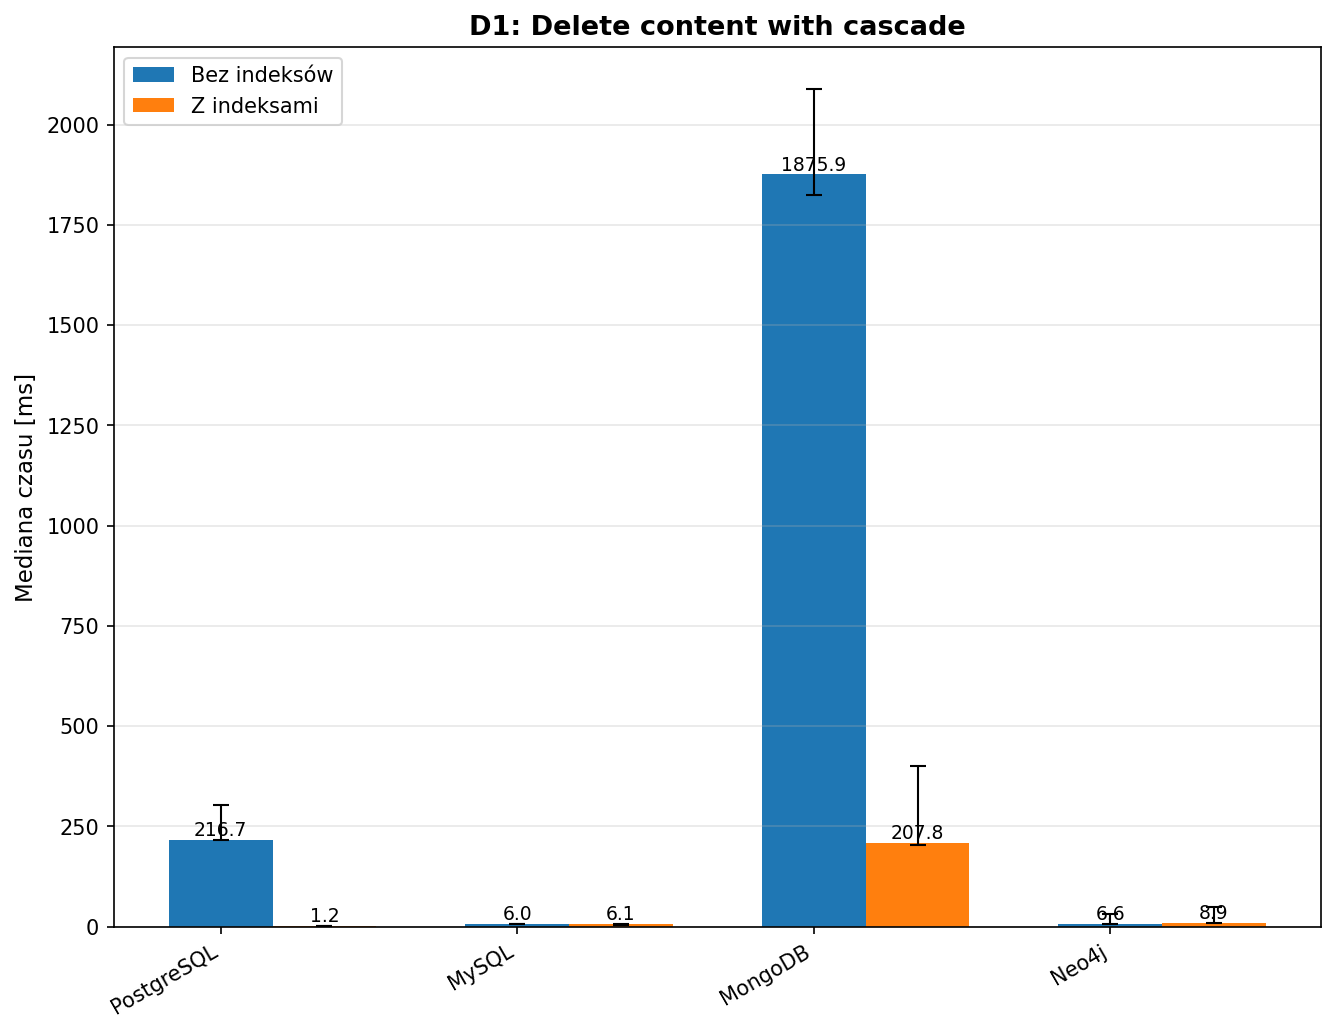
\includegraphics[width=0.8\textwidth]{charts/large/chart_D1.png}
    \caption{D1 -- Usunięcie treści z kaskadą}
\end{figure}

Skala potęguje efekt indeksu na FK. PostgreSQL bez indeksu --
\textbf{217~ms}, z indeksem \emph{1.2~ms} (180-krotne przyspieszenie).
MongoDB bez indeksu 1.9~sekundy(!), z indeksem 208~ms (9×).
Neo4j 7--9~ms niezależnie od wariantu -- relacje są wskaźnikami,
więc kaskada to natychmiastowe odnalezienie sąsiadów. MySQL stabilnie
6~ms (FK index nieusuwalny). Wniosek: dla tabel ze związkami
kaskadowymi indeks na kluczu obcym jest \emph{absolutną koniecznością}
-- bez niego każde usunięcie staje się skanem powiązanych tabel.

\subsubsection{D4: Usunięcie pozycji z listy}
\begin{figure}[H]
    \centering
    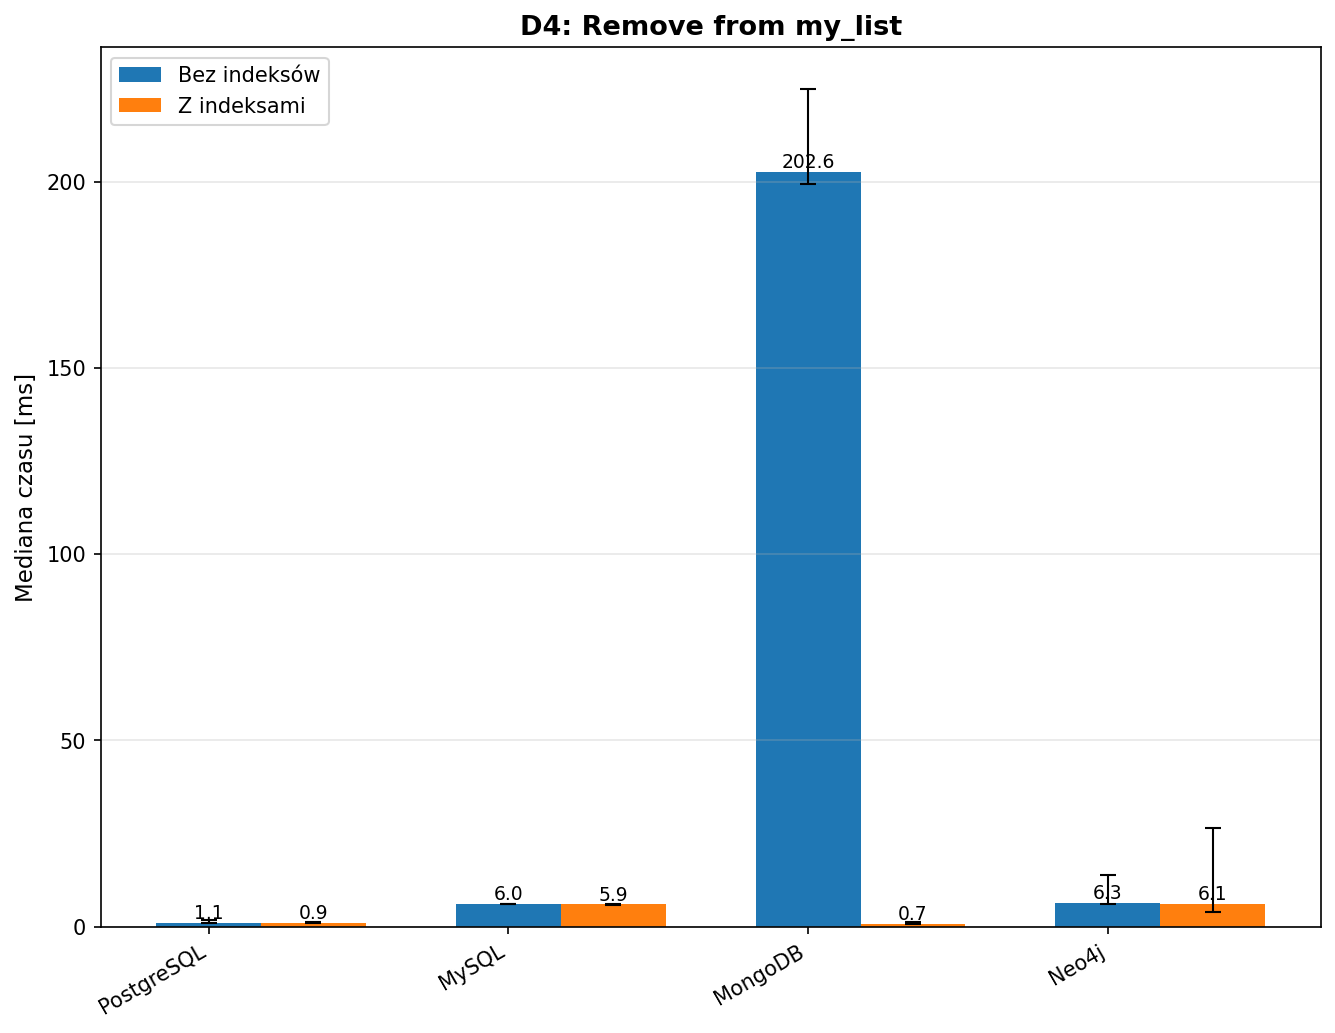
\includegraphics[width=0.8\textwidth]{charts/large/chart_D4.png}
    \caption{D4 -- Usunięcie pozycji z listy}
\end{figure}

MongoDB bez indeksu eskaluje do \textbf{202~ms} (z 20~ms na
\emph{small}) -- klasyczne liniowe skalowanie skanu kolekcji.
Z indeksem 0.7~ms -- \emph{286-krotna} różnica. To najsilniej
skalujący się dowód wartości indeksu w całej pracy. PostgreSQL
i Neo4j stałe poniżej 6~ms, MySQL stałe 6~ms. Operacja prosta,
ale dramatycznie różna w zachowaniu między modelem indeksowanym
a nieindeksowanym.

\subsubsection{D6: Masowe usunięcie nieaktywnych użytkowników}
\begin{figure}[H]
    \centering
    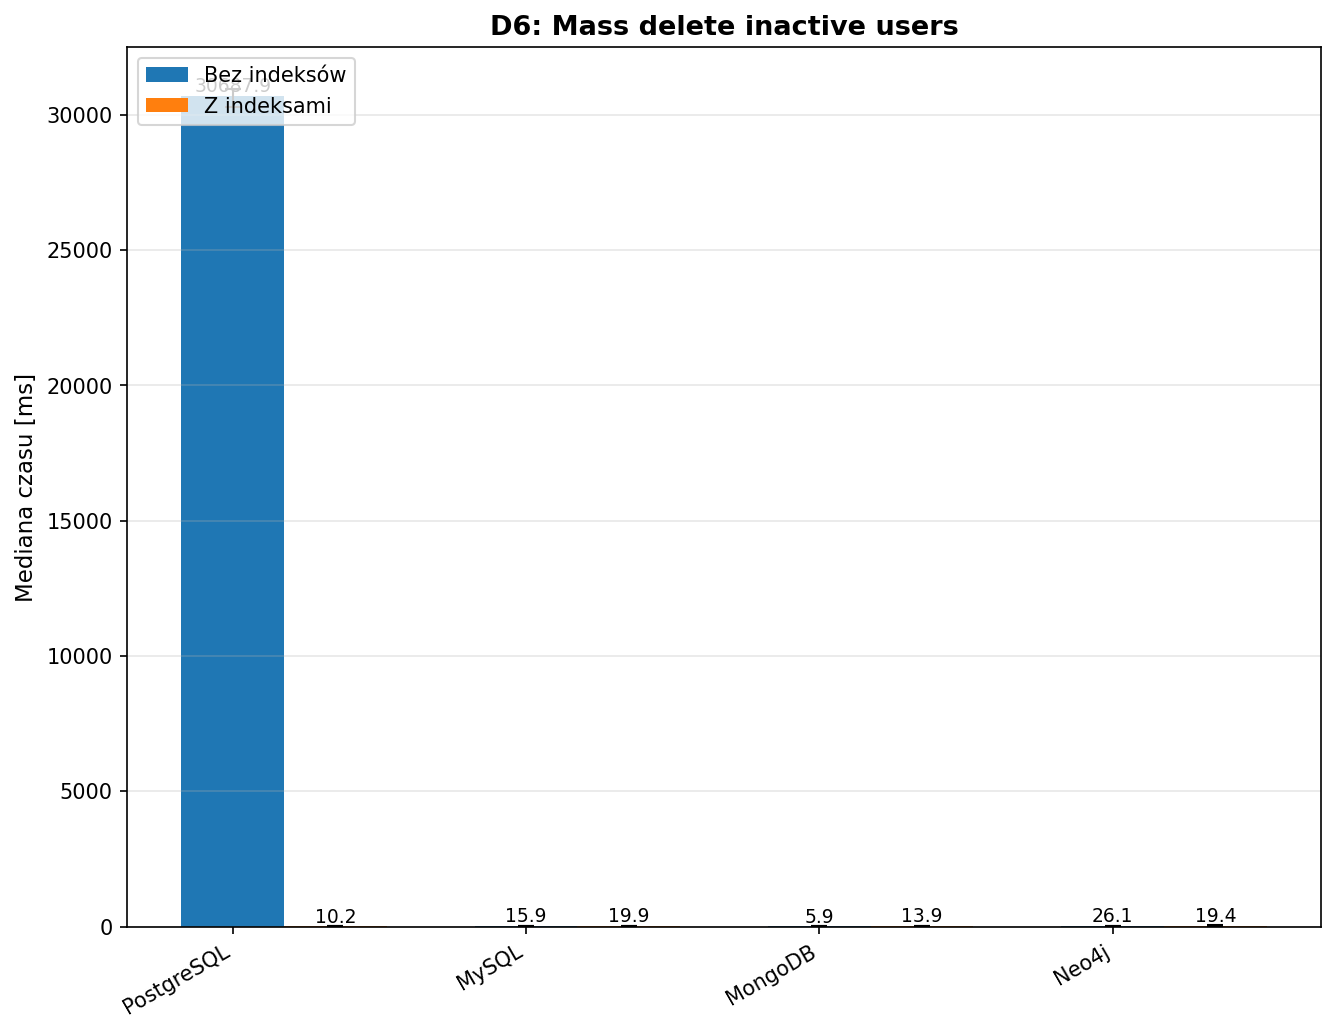
\includegraphics[width=0.8\textwidth]{charts/large/chart_D6.png}
    \caption{D6 -- Masowe usunięcie nieaktywnych użytkowników}
\end{figure}

Najbardziej spektakularny wynik całej pracy. PostgreSQL bez indeksu
na \texttt{users.status}: \textbf{30.7 sekundy}. Z indeksem:
\emph{10~milisekund}. To \textbf{3000-krotne} przyspieszenie --
indeks zmienia operację, która jest praktycznie niewykonalna
w produkcji w operację w czasie reakcji aplikacji webowej. MongoDB
i Neo4j również zyskują (5.9 → 13.9~ms i 26 → 19~ms odpowiednio),
ale bez tej dramatycznej skali. MySQL stabilnie 16--20~ms. Ten
scenariusz powinien być \emph{centralnym argumentem} pracy:
różnica trzy rzędów wielkości to nie kosmetyka, to różnica między
,,można uruchomić'' a ,,nie wolno wykonać''.

% -------------------------------------------------------
% UPDATE
% -------------------------------------------------------

\subsubsection{U2: Przeliczenie średniej oceny}
\begin{figure}[H]
    \centering
    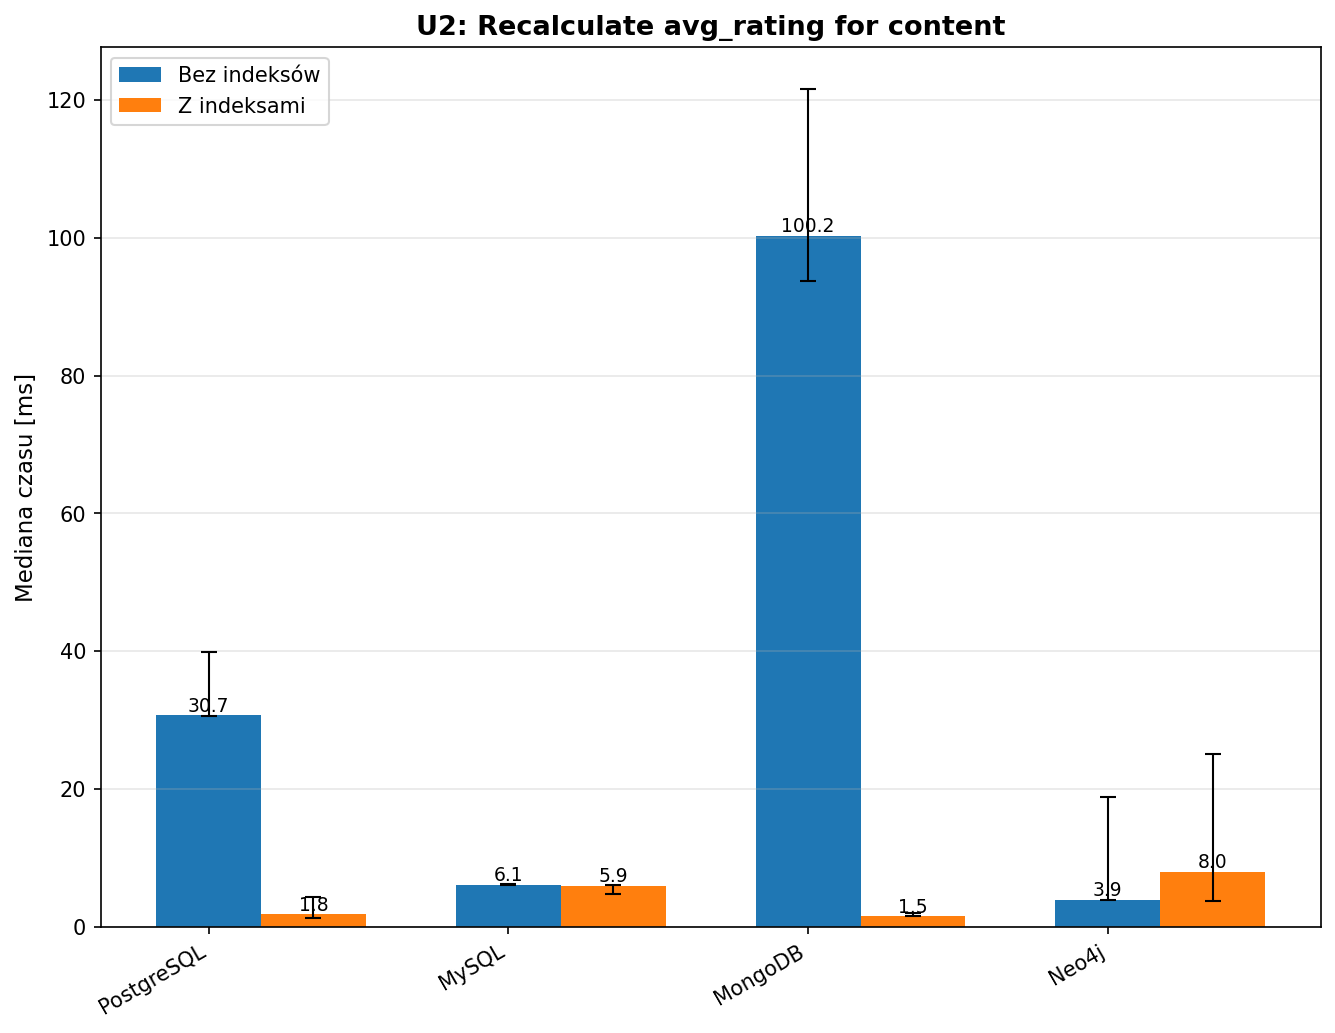
\includegraphics[width=0.8\textwidth]{charts/large/chart_U2.png}
    \caption{U2 -- Przeliczenie średniej oceny}
\end{figure}

Wzorzec ze \emph{small} i \emph{medium} się skaluje, ale kontrast
rośnie. PostgreSQL bez indeksu 30.7~ms (był 8.8~ms na \emph{medium}),
z indeksem 1.8~ms. MongoDB bez indeksu 100~ms, z indeksem 1.5~ms
(67×). MySQL i Neo4j stabilne 6 i 4--8~ms. Pojedynczy \texttt{UPDATE}
po agregacie -- kontrast między ,,znalezieniem wiersza'' z indeksem
a ,,znalezieniem wiersza'' przez skan jest tym wyraźniejszy, im więcej
wierszy do przeskanowania. Indeks działa idealnie zgodnie
z hipotezą.

\subsubsection{U3: Masowa zmiana planu subskrypcji}
\begin{figure}[H]
    \centering
    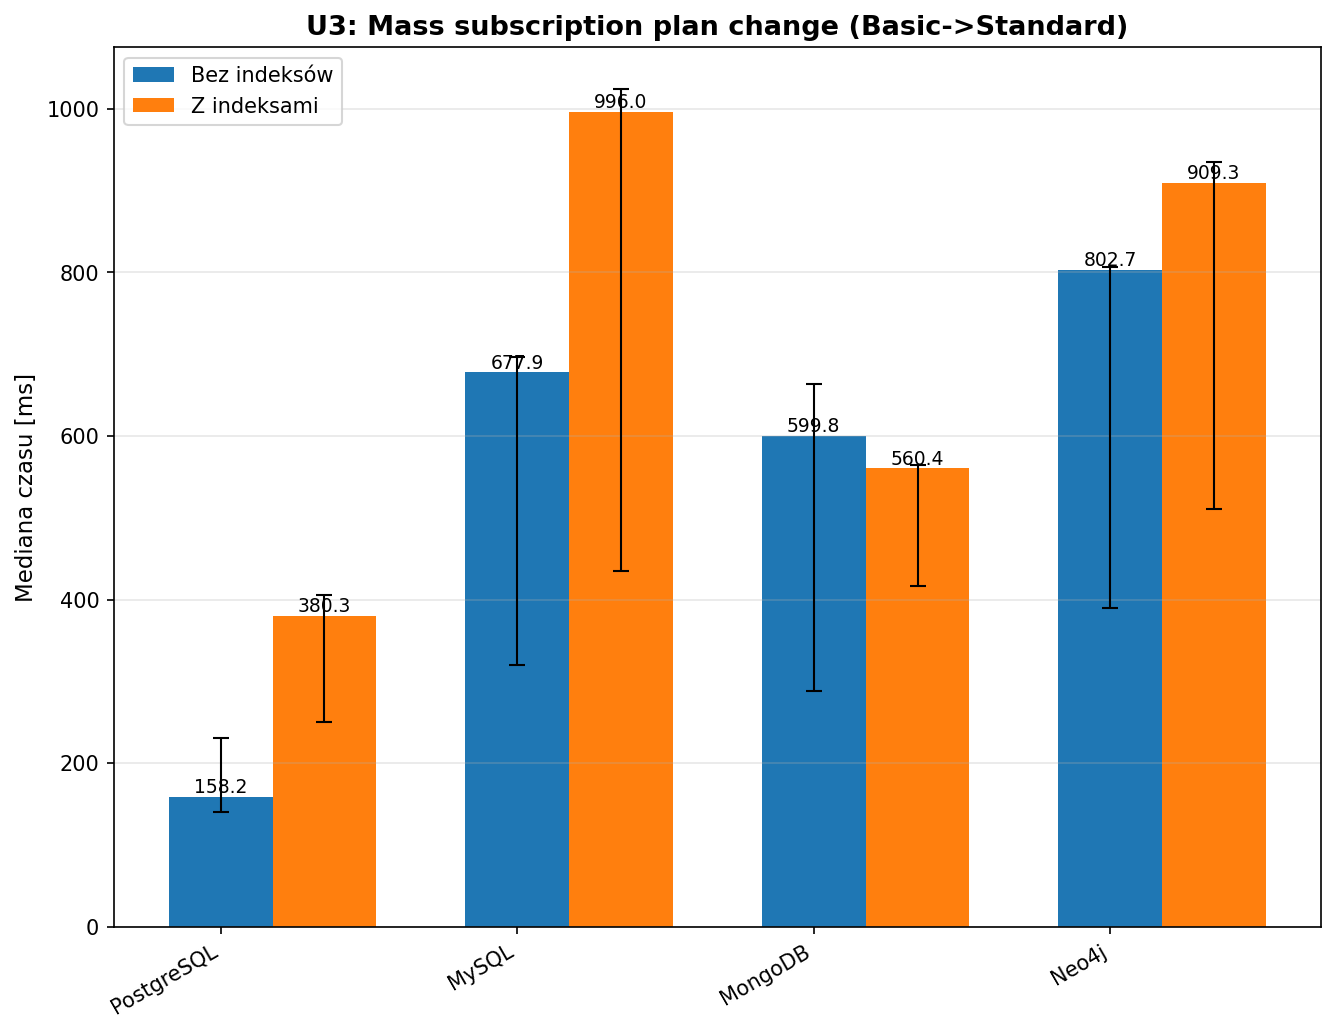
\includegraphics[width=0.8\textwidth]{charts/large/chart_U3.png}
    \caption{U3 -- Masowa zmiana planu subskrypcji}
\end{figure}

Koszt utrzymania indeksów przy modyfikacji wierszy osiąga tu
maksimum. PostgreSQL bez indeksu
158~ms, z indeksem \emph{380~ms} -- \textbf{2.4-krotne pogorszenie}.
MySQL 678 → 996~ms (1.5×), Neo4j 803 → 909~ms (1.1×), MongoDB
599 → 560~ms (lekko lepiej). Operacja modyfikuje pole \texttt{plan\_name}
na milionach wierszy -- każda zmiana wymusza przepisanie wpisu
w indeksie złożonym \texttt{(status, plan\_name)}. To jest
\emph{koronny dowód drugiej części hipotezy}: dla masowych
\texttt{UPDATE}-ów na kolumnach indeksowanych obecność indeksu
jest \emph{kosztem}, nie zyskiem. Razem z D6 ten scenariusz
domyka pełną diagnozę: indeks może być najlepszym przyjacielem
albo najgorszym wrogiem, w zależności od tego, czy operacja
\emph{czyta} czy \emph{pisze} po indeksowanej kolumnie.

% -------------------------------------------------------


\section{Analiza wyników i weryfikacja hipotezy}

Hipoteza zakłada, że zastosowanie indeksów znacząco poprawia wydajność
operacji SELECT kosztem spadku wydajności operacji INSERT i UPDATE.

Poniższe heatmapy przedstawiają stosunek czasu wykonania z indeksami
do czasu bez indeksów dla każdego scenariusza i każdej bazy danych.
Kolor zielony oznacza że indeks przyspieszył operację (wartość poniżej 1.0),
kolor czerwony że ją spowolnił (wartość powyżej 1.0).
 
\begin{figure}[H]
    \centering
    
\includegraphics[width=1.0\textwidth]{charts/small/index_heatmap_small.png}
    \caption{Mapa cieplna wpływu indeksów na wydajność -- wolumen small}
\end{figure}
 
\begin{figure}[H]
    \centering
    
\includegraphics[width=1.0\textwidth]{charts/medium/index_heatmap_medium.png}
    \caption{Mapa cieplna wpływu indeksów na wydajność -- wolumen medium}
\end{figure}
 
\begin{figure}[H]
    \centering
    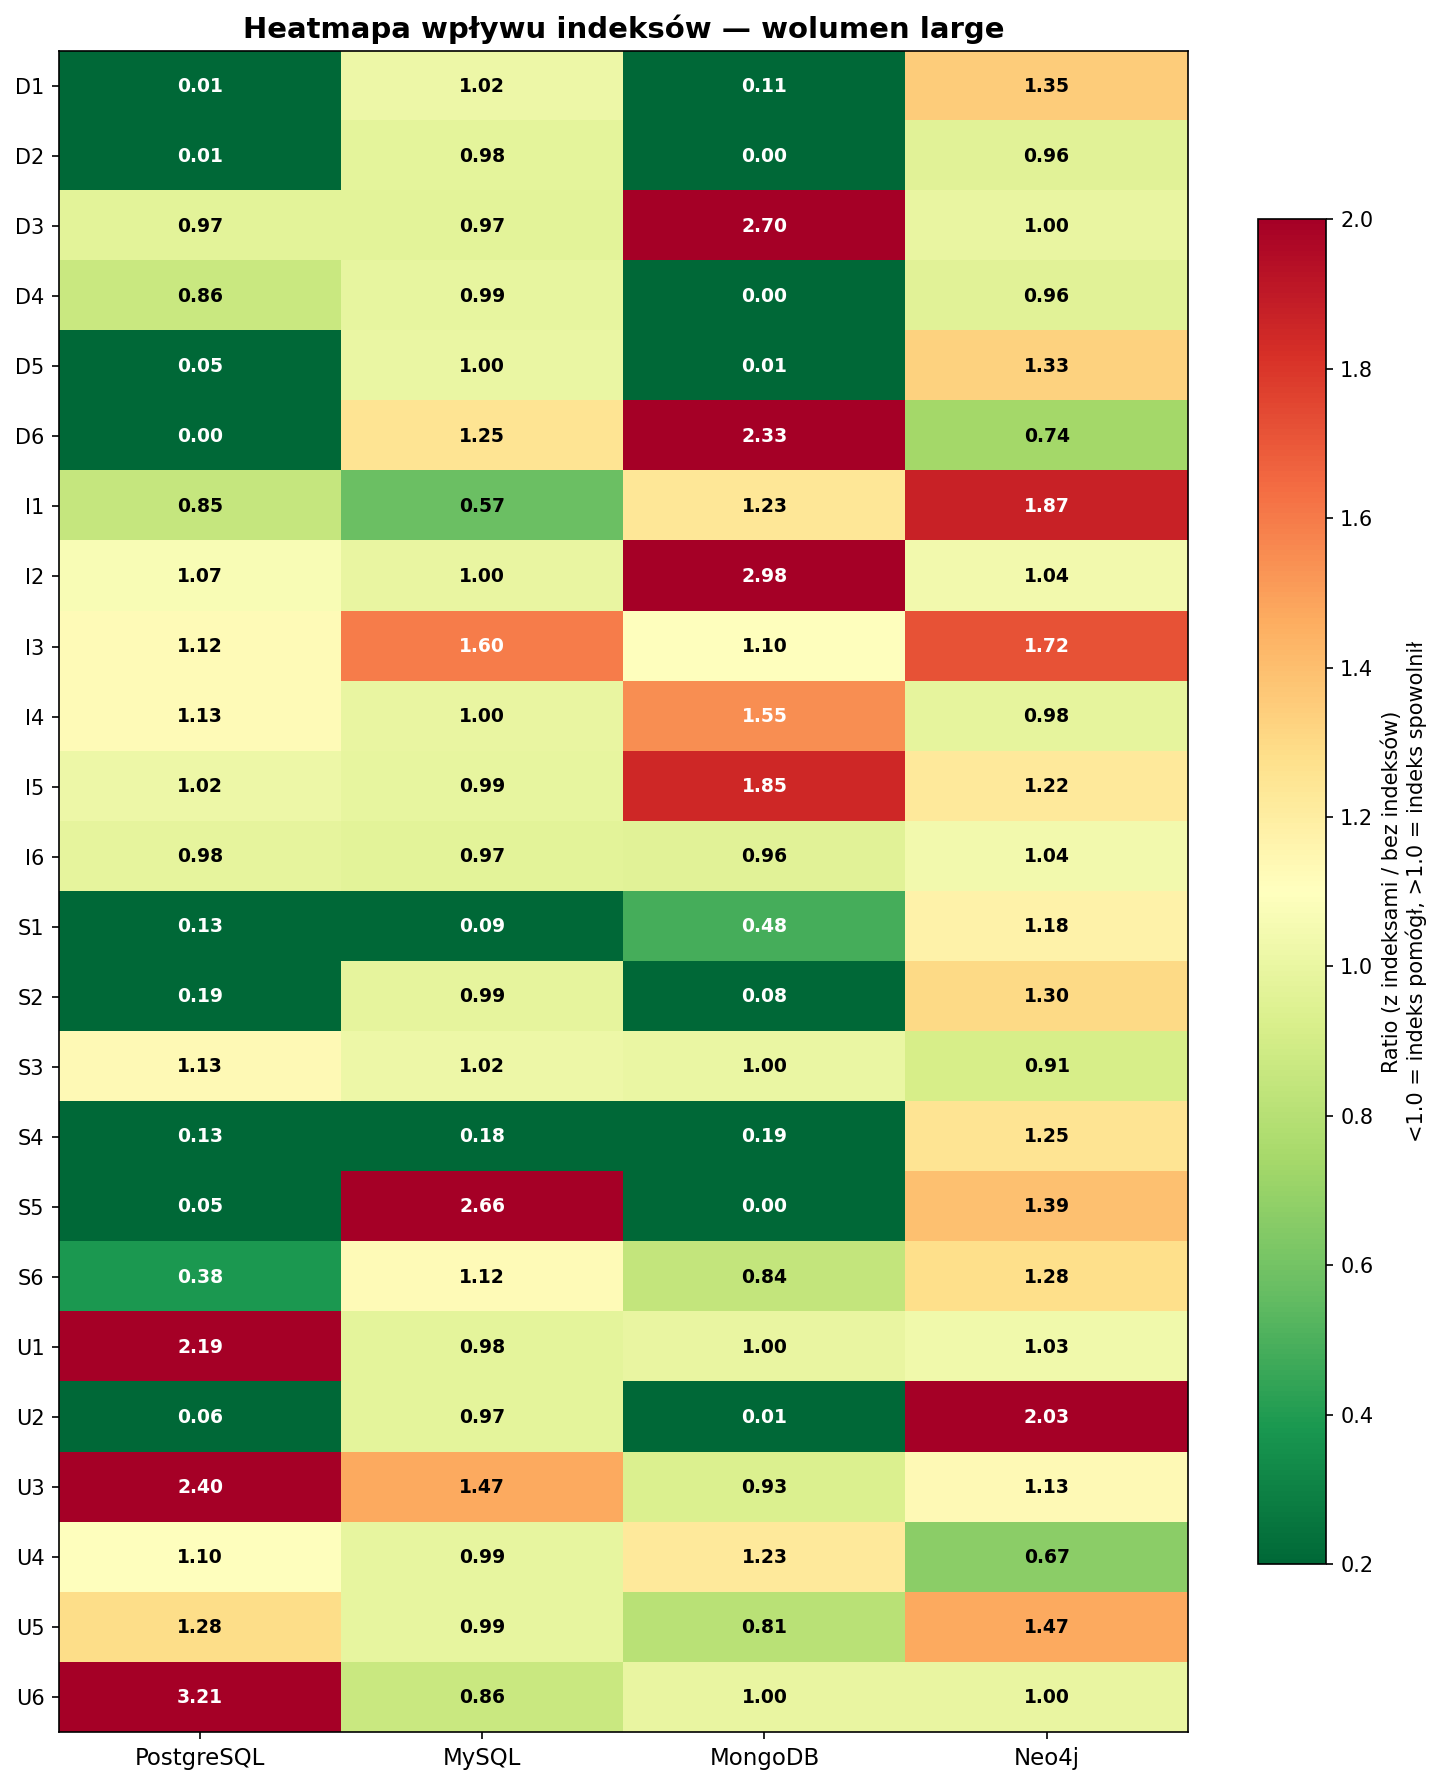
\includegraphics[width=1.0\textwidth]{charts/large/index_heatmap_large.png}
    \caption{Mapa cieplna wpływu indeksów na wydajność -- wolumen large}
\end{figure}
% -------------------------------------------------------
\section{Podsumowanie}

% -------------------------------------------------------
\appendix
\section{Dodatek -- pozostałe wykresy benchmarków}
% -------------------------------------------------------
% Pozostałe wykresy benchmarków (scenariusze nieomówione w sekcji głównej)
% -------------------------------------------------------

\subsection{Wolumen small - 500 000 rekordów}

% -------------------------------------------------------
% INSERT
% -------------------------------------------------------

\subsubsection{I1: Rejestracja użytkownika}
\begin{figure}[H]
    \centering
    
\includegraphics[width=0.8\textwidth]{charts/small/chart_I1.png}
    \caption{I1 -- Rejestracja użytkownika (small)}
\end{figure}

\subsubsection{I4: Batch insert płatności}
\begin{figure}[H]
    \centering
    
\includegraphics[width=0.8\textwidth]{charts/small/chart_I4.png}
    \caption{I4 -- Batch insert płatności (small)}
\end{figure}

\subsubsection{I5: Oceny z przeliczeniem średniej}
\begin{figure}[H]
    \centering
    
\includegraphics[width=0.8\textwidth]{charts/small/chart_I5.png}
    \caption{I5 -- Oceny z przeliczeniem średniej oceny (small)}
\end{figure}

\subsubsection{I6: Import osób z powiązaniami}
\begin{figure}[H]
    \centering
    
\includegraphics[width=0.8\textwidth]{charts/small/chart_I6.png}
    \caption{I6 -- Import osób z powiązaniami (small)}
\end{figure}

% -------------------------------------------------------
% SELECT
% -------------------------------------------------------

\subsubsection{S1: Strona główna}
\begin{figure}[H]
    \centering
    
\includegraphics[width=0.8\textwidth]{charts/small/chart_S1.png}
    \caption{S1 -- Strona główna (small)}
\end{figure}

\subsubsection{S5: Historia oglądania profilu}
\begin{figure}[H]
    \centering
    
\includegraphics[width=0.8\textwidth]{charts/small/chart_S5.png}
    \caption{S5 -- Historia oglądania profilu (small)}
\end{figure}

\subsubsection{S6: Filmografia osoby}
\begin{figure}[H]
    \centering
    
\includegraphics[width=0.8\textwidth]{charts/small/chart_S6.png}
    \caption{S6 -- Filmografia osoby (small)}
\end{figure}

% -------------------------------------------------------
% DELETE
% -------------------------------------------------------

\subsubsection{D2: Usunięcie profilu z historią}
\begin{figure}[H]
    \centering
    
\includegraphics[width=0.8\textwidth]{charts/small/chart_D2.png}
    \caption{D2 -- Usunięcie profilu z historią (small)}
\end{figure}

\subsubsection{D3: Czyszczenie starych ocen}
\begin{figure}[H]
    \centering
    
\includegraphics[width=0.8\textwidth]{charts/small/chart_D3.png}
    \caption{D3 -- Czyszczenie starych ocen (small)}
\end{figure}

\subsubsection{D5: Usunięcie subskrypcji z płatnościami}
\begin{figure}[H]
    \centering
    
\includegraphics[width=0.8\textwidth]{charts/small/chart_D5.png}
    \caption{D5 -- Usunięcie subskrypcji z płatnościami (small)}
\end{figure}

% -------------------------------------------------------
% UPDATE
% -------------------------------------------------------

\subsubsection{U1: Aktualizacja postępu oglądania}
\begin{figure}[H]
    \centering
    
\includegraphics[width=0.8\textwidth]{charts/small/chart_U1.png}
    \caption{U1 -- Aktualizacja postępu oglądania (small)}
\end{figure}

\subsubsection{U4: Aktualizacja danych użytkownika}
\begin{figure}[H]
    \centering
    
\includegraphics[width=0.8\textwidth]{charts/small/chart_U4.png}
    \caption{U4 -- Aktualizacja danych użytkownika (small)}
\end{figure}

\subsubsection{U5: Oznaczenie treści jako nieaktywnej}
\begin{figure}[H]
    \centering
    
\includegraphics[width=0.8\textwidth]{charts/small/chart_U5.png}
    \caption{U5 -- Oznaczenie treści jako nieaktywnej (small)}
\end{figure}

\subsubsection{U6: Masowa aktualizacja wskaźnika popularności}
\begin{figure}[H]
    \centering
    
\includegraphics[width=0.8\textwidth]{charts/small/chart_U6.png}
    \caption{U6 -- Masowa aktualizacja wskaźnika popularności (small)}
\end{figure}


\subsection{Wolumen medium - 1 000 000 rekordów}

% -------------------------------------------------------
% INSERT
% -------------------------------------------------------

\subsubsection{I1: Rejestracja użytkownika}
\begin{figure}[H]
    \centering
    
\includegraphics[width=0.8\textwidth]{charts/medium/chart_I1.png}
    \caption{I1 -- Rejestracja użytkownika (medium)}
\end{figure}

\subsubsection{I4: Batch insert płatności}
\begin{figure}[H]
    \centering
    
\includegraphics[width=0.8\textwidth]{charts/medium/chart_I4.png}
    \caption{I4 -- Batch insert płatności (medium)}
\end{figure}

\subsubsection{I5: Oceny z przeliczeniem średniej}
\begin{figure}[H]
    \centering
    
\includegraphics[width=0.8\textwidth]{charts/medium/chart_I5.png}
    \caption{I5 -- Oceny z przeliczeniem średniej oceny (medium)}
\end{figure}

\subsubsection{I6: Import osób z powiązaniami}
\begin{figure}[H]
    \centering
    
\includegraphics[width=0.8\textwidth]{charts/medium/chart_I6.png}
    \caption{I6 -- Import osób z powiązaniami (medium)}
\end{figure}

% -------------------------------------------------------
% SELECT
% -------------------------------------------------------

\subsubsection{S1: Strona główna}
\begin{figure}[H]
    \centering
    
\includegraphics[width=0.8\textwidth]{charts/medium/chart_S1.png}
    \caption{S1 -- Strona główna (medium)}
\end{figure}

\subsubsection{S5: Historia oglądania profilu}
\begin{figure}[H]
    \centering
    
\includegraphics[width=0.8\textwidth]{charts/medium/chart_S5.png}
    \caption{S5 -- Historia oglądania profilu (medium)}
\end{figure}

\subsubsection{S6: Filmografia osoby}
\begin{figure}[H]
    \centering
    
\includegraphics[width=0.8\textwidth]{charts/medium/chart_S6.png}
    \caption{S6 -- Filmografia osoby (medium)}
\end{figure}

% -------------------------------------------------------
% DELETE
% -------------------------------------------------------

\subsubsection{D2: Usunięcie profilu z historią}
\begin{figure}[H]
    \centering
    
\includegraphics[width=0.8\textwidth]{charts/medium/chart_D2.png}
    \caption{D2 -- Usunięcie profilu z historią (medium)}
\end{figure}

\subsubsection{D3: Czyszczenie starych ocen}
\begin{figure}[H]
    \centering
    
\includegraphics[width=0.8\textwidth]{charts/medium/chart_D3.png}
    \caption{D3 -- Czyszczenie starych ocen (medium)}
\end{figure}

\subsubsection{D5: Usunięcie subskrypcji z płatnościami}
\begin{figure}[H]
    \centering
    
\includegraphics[width=0.8\textwidth]{charts/medium/chart_D5.png}
    \caption{D5 -- Usunięcie subskrypcji z płatnościami (medium)}
\end{figure}

% -------------------------------------------------------
% UPDATE
% -------------------------------------------------------

\subsubsection{U1: Aktualizacja postępu oglądania}
\begin{figure}[H]
    \centering
    
\includegraphics[width=0.8\textwidth]{charts/medium/chart_U1.png}
    \caption{U1 -- Aktualizacja postępu oglądania (medium)}
\end{figure}

\subsubsection{U4: Aktualizacja danych użytkownika}
\begin{figure}[H]
    \centering
    
\includegraphics[width=0.8\textwidth]{charts/medium/chart_U4.png}
    \caption{U4 -- Aktualizacja danych użytkownika (medium)}
\end{figure}

\subsubsection{U5: Oznaczenie treści jako nieaktywnej}
\begin{figure}[H]
    \centering
    
\includegraphics[width=0.8\textwidth]{charts/medium/chart_U5.png}
    \caption{U5 -- Oznaczenie treści jako nieaktywnej (medium)}
\end{figure}

\subsubsection{U6: Masowa aktualizacja wskaźnika popularności}
\begin{figure}[H]
    \centering
    
\includegraphics[width=0.8\textwidth]{charts/medium/chart_U6.png}
    \caption{U6 -- Masowa aktualizacja wskaźnika popularności (medium)}
\end{figure}


\subsection{Wolumen large - 10 000 000 rekordów}

% -------------------------------------------------------
% INSERT
% -------------------------------------------------------

\subsubsection{I1: Rejestracja użytkownika}
\begin{figure}[H]
    \centering
    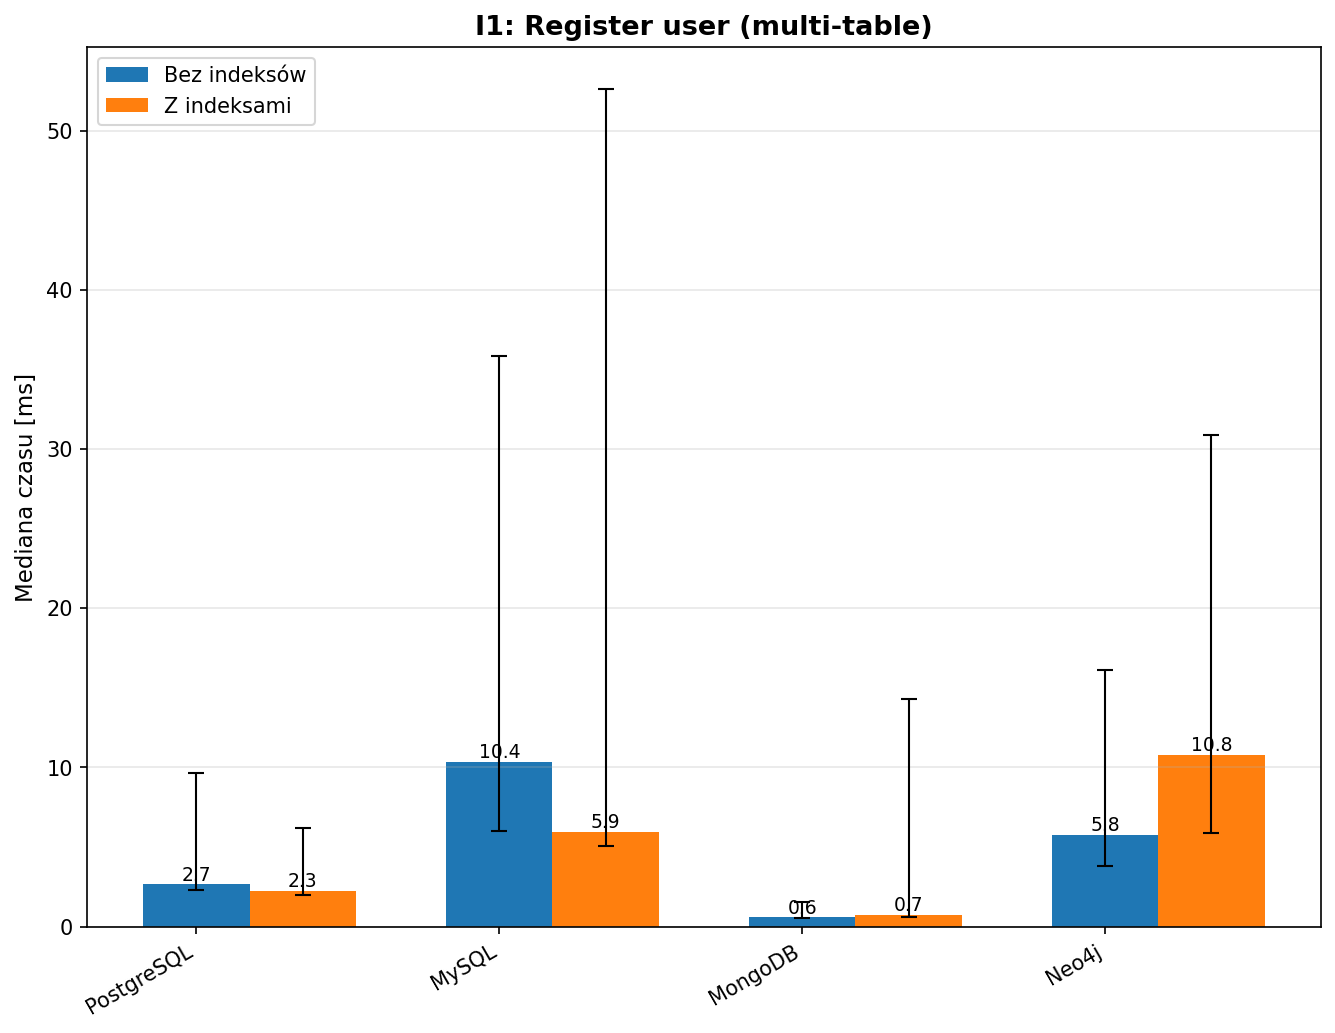
\includegraphics[width=0.8\textwidth]{charts/large/chart_I1.png}
    \caption{I1 -- Rejestracja użytkownika (large)}
\end{figure}

\subsubsection{I4: Batch insert płatności}
\begin{figure}[H]
    \centering
    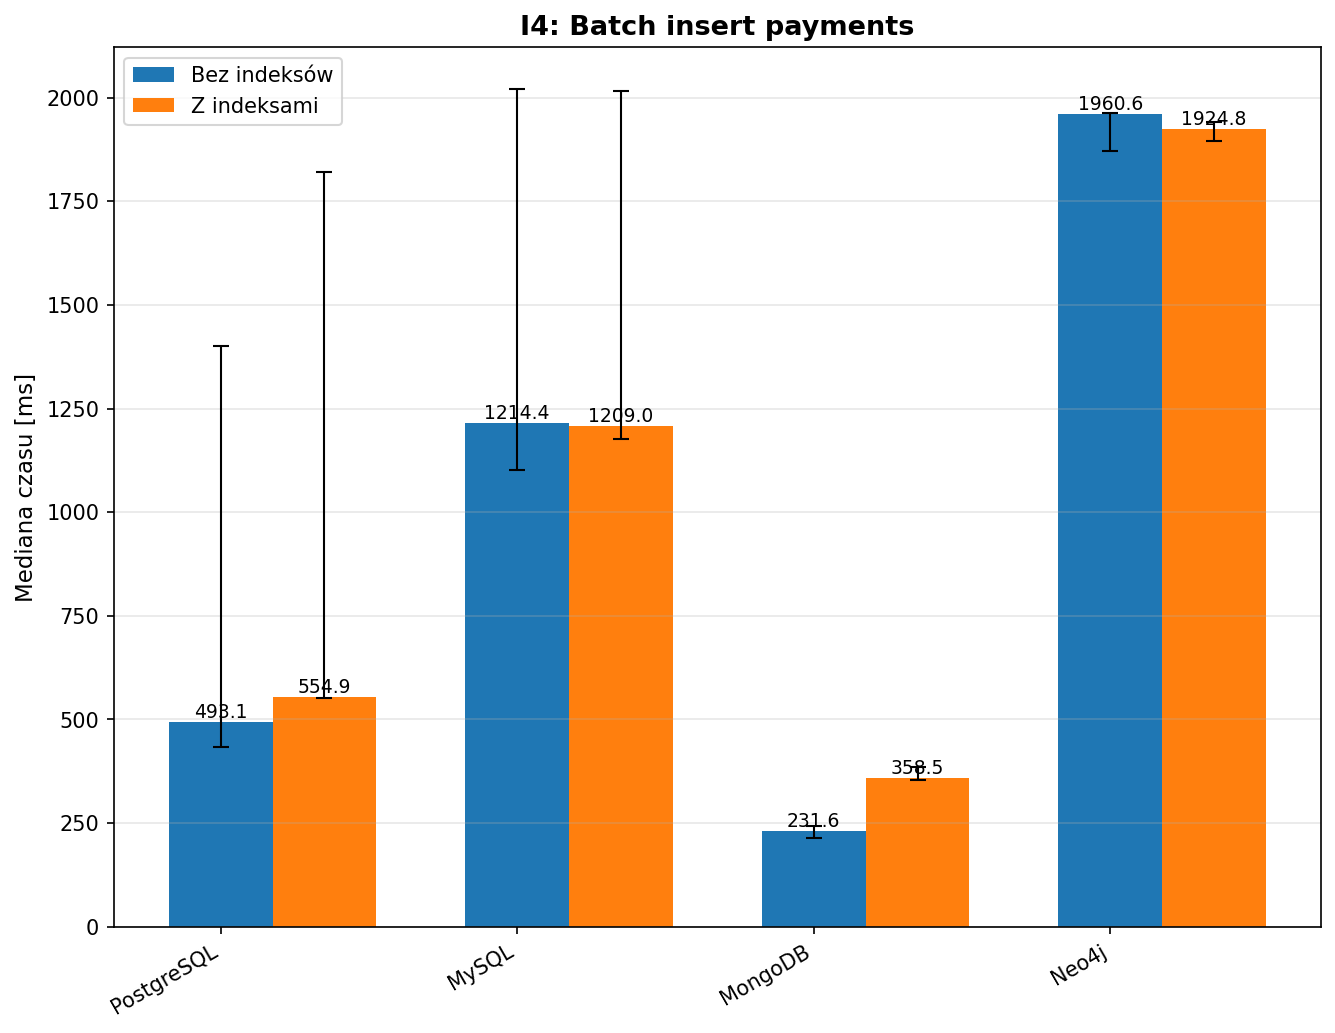
\includegraphics[width=0.8\textwidth]{charts/large/chart_I4.png}
    \caption{I4 -- Batch insert płatności (large)}
\end{figure}

\subsubsection{I5: Oceny z przeliczeniem średniej}
\begin{figure}[H]
    \centering
    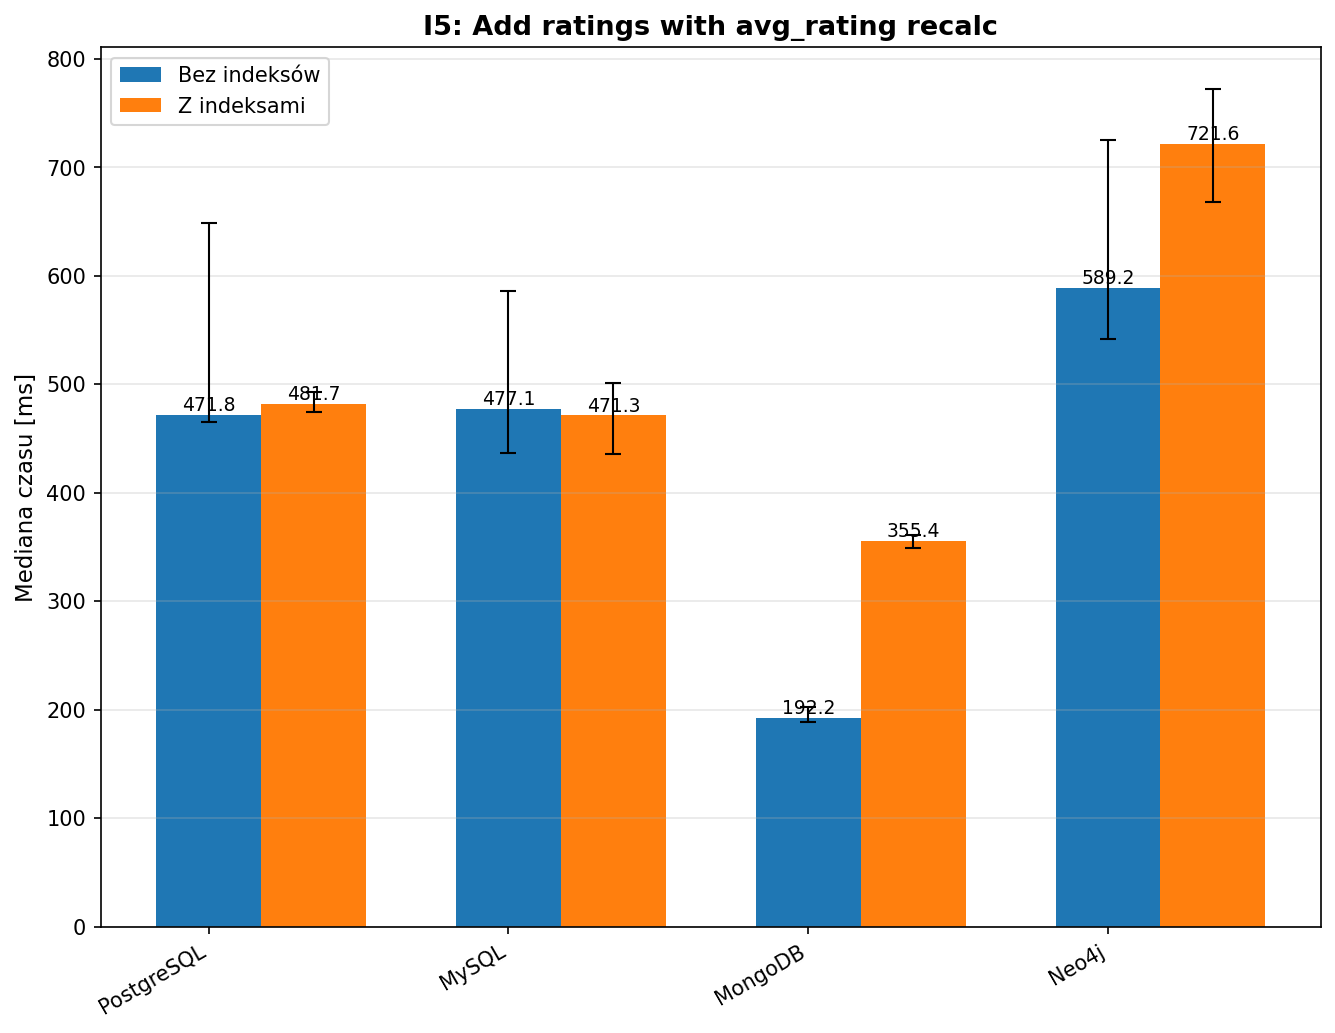
\includegraphics[width=0.8\textwidth]{charts/large/chart_I5.png}
    \caption{I5 -- Oceny z przeliczeniem średniej oceny (large)}
\end{figure}

\subsubsection{I6: Import osób z powiązaniami}
\begin{figure}[H]
    \centering
    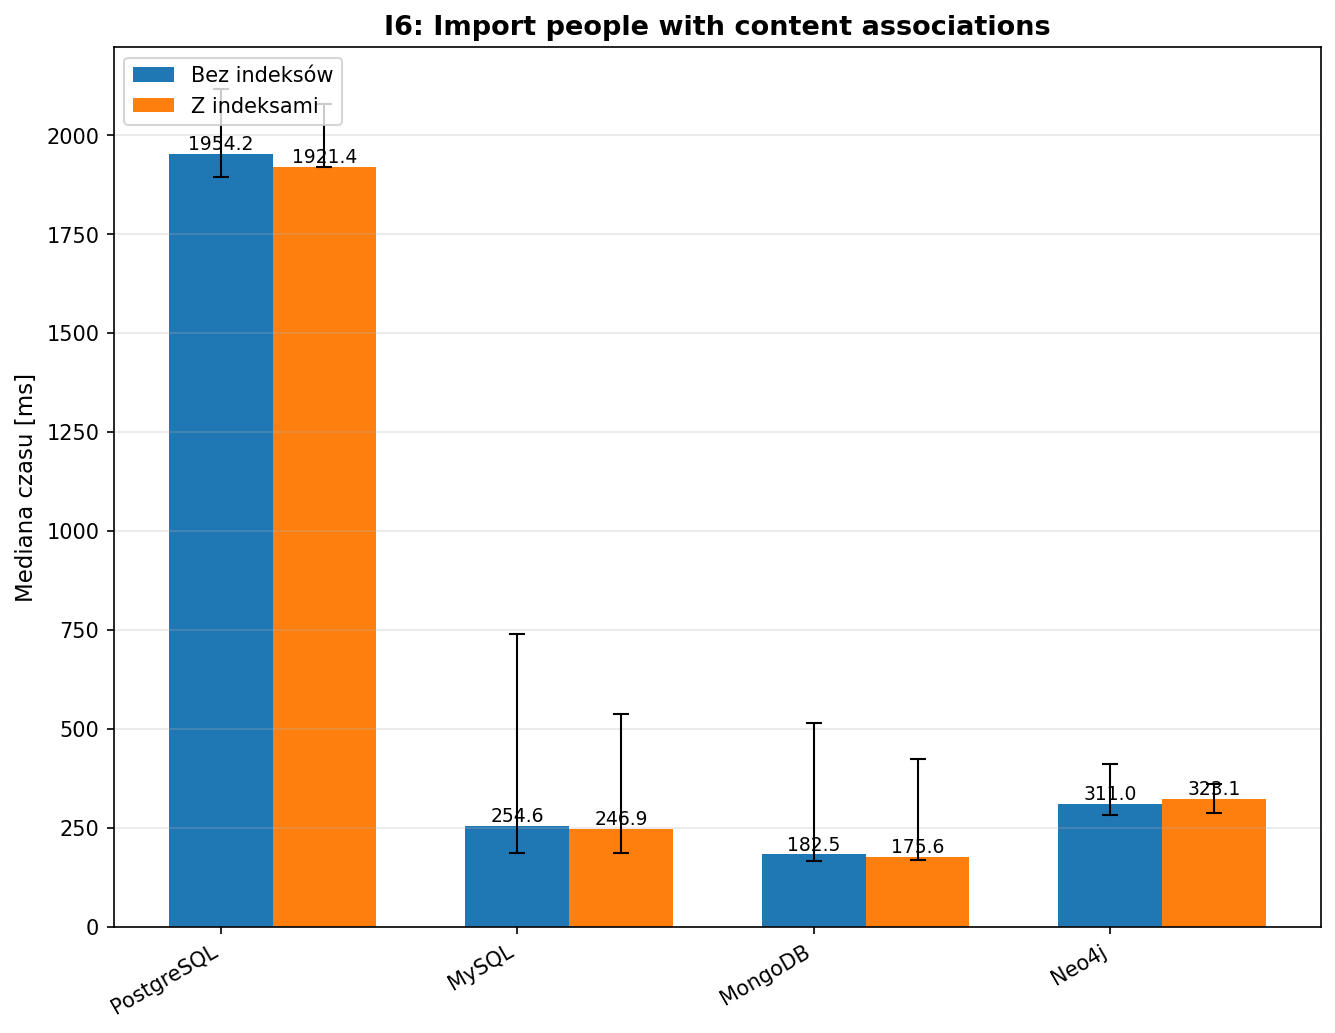
\includegraphics[width=0.8\textwidth]{charts/large/chart_I6.png}
    \caption{I6 -- Import osób z powiązaniami (large)}
\end{figure}

% -------------------------------------------------------
% SELECT
% -------------------------------------------------------

\subsubsection{S1: Strona główna}
\begin{figure}[H]
    \centering
    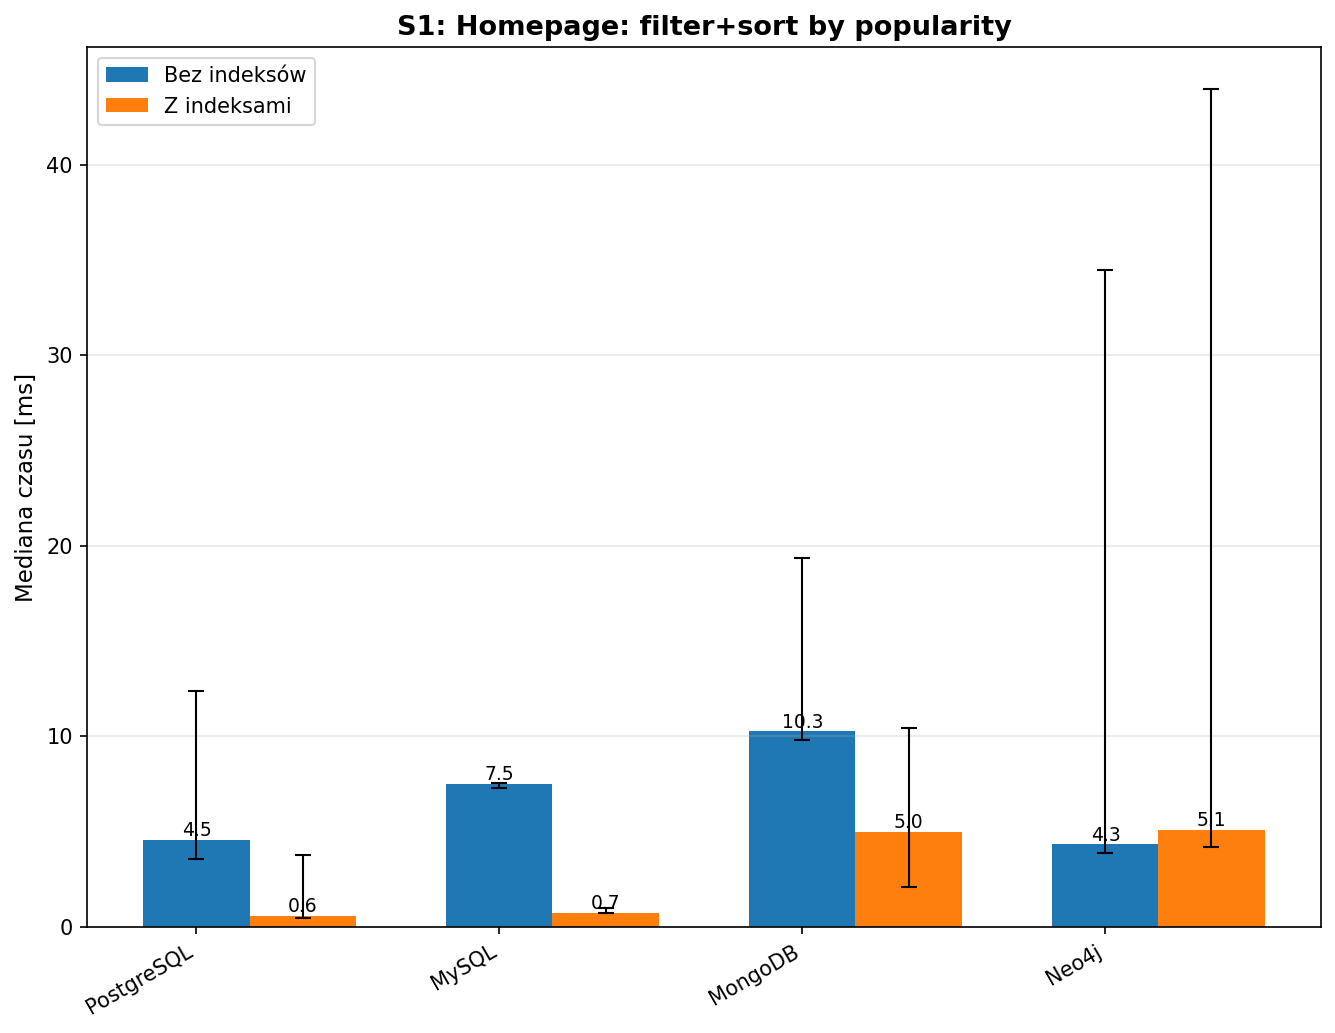
\includegraphics[width=0.8\textwidth]{charts/large/chart_S1.png}
    \caption{S1 -- Strona główna (large)}
\end{figure}

\subsubsection{S5: Historia oglądania profilu}
\begin{figure}[H]
    \centering
    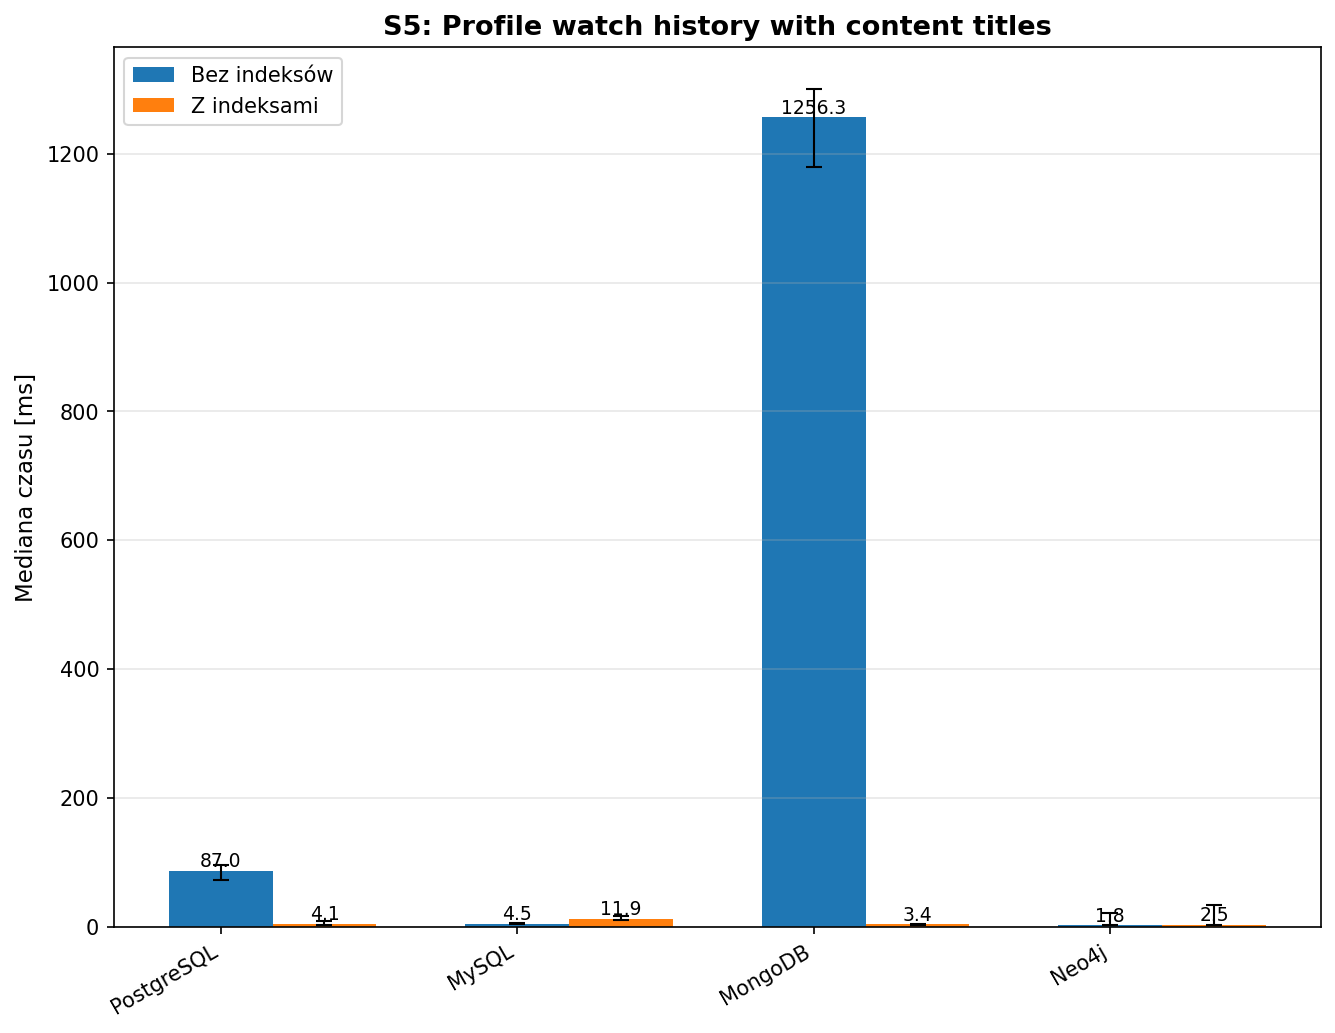
\includegraphics[width=0.8\textwidth]{charts/large/chart_S5.png}
    \caption{S5 -- Historia oglądania profilu (large)}
\end{figure}

\subsubsection{S6: Filmografia osoby}
\begin{figure}[H]
    \centering
    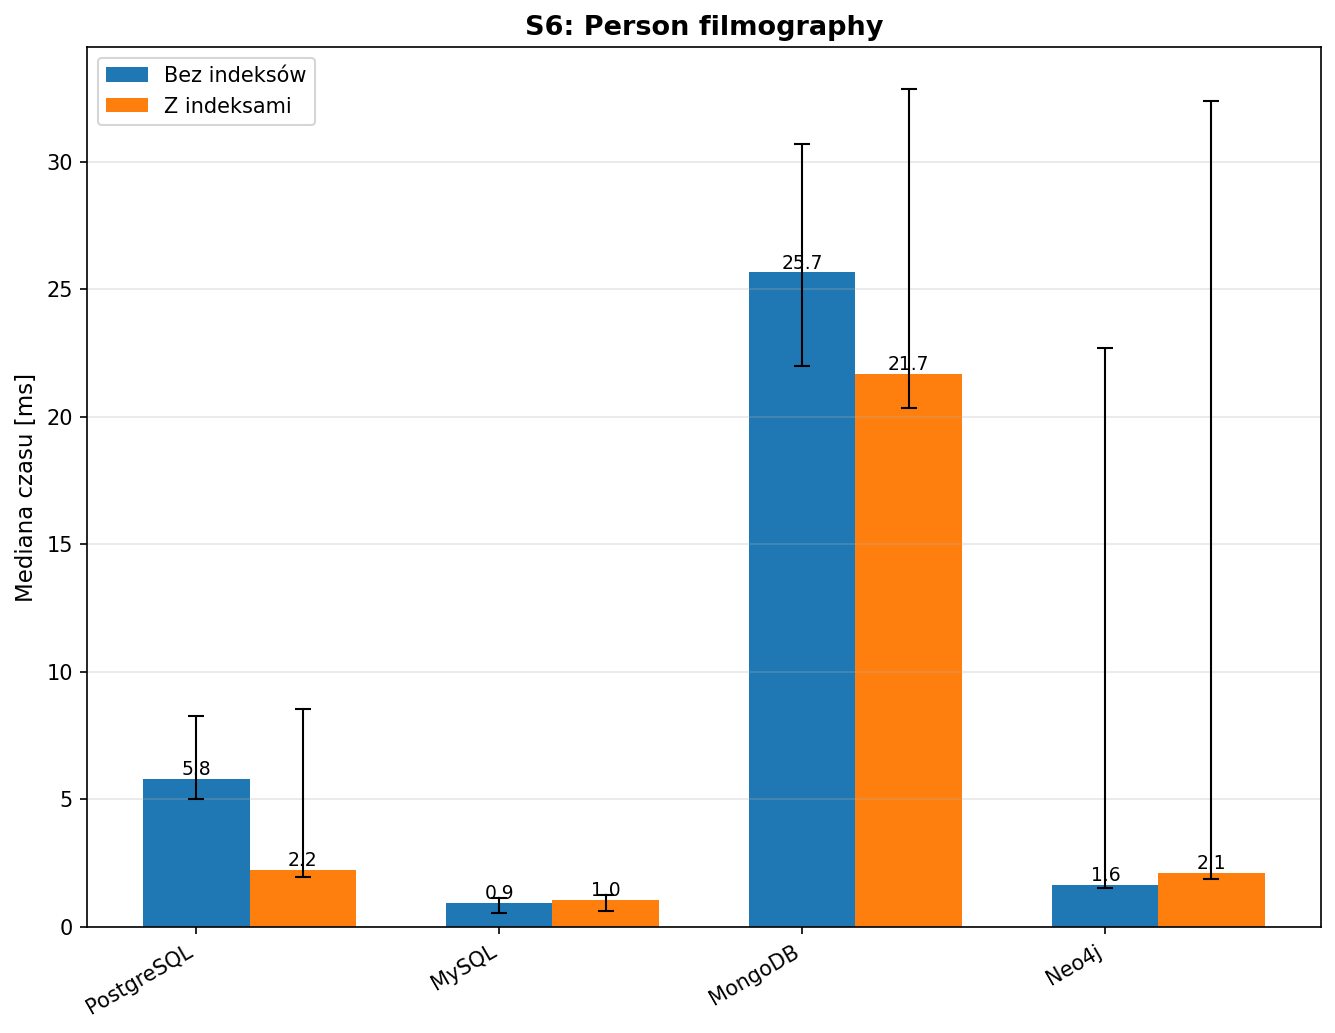
\includegraphics[width=0.8\textwidth]{charts/large/chart_S6.png}
    \caption{S6 -- Filmografia osoby (large)}
\end{figure}

% -------------------------------------------------------
% DELETE
% -------------------------------------------------------

\subsubsection{D2: Usunięcie profilu z historią}
\begin{figure}[H]
    \centering
    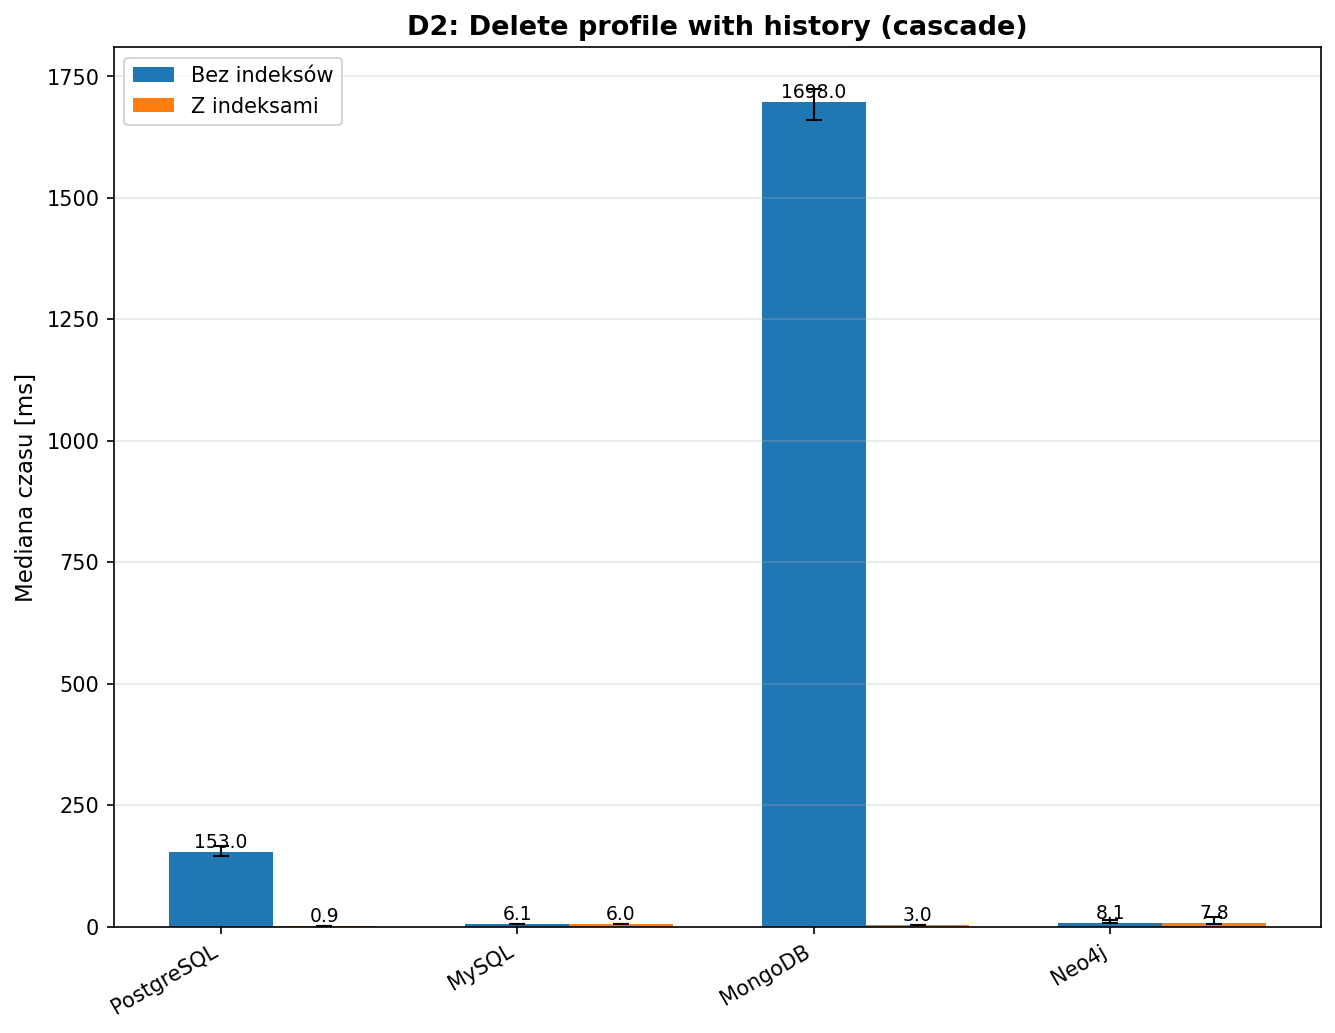
\includegraphics[width=0.8\textwidth]{charts/large/chart_D2.png}
    \caption{D2 -- Usunięcie profilu z historią (large)}
\end{figure}

\subsubsection{D3: Czyszczenie starych ocen}
\begin{figure}[H]
    \centering
    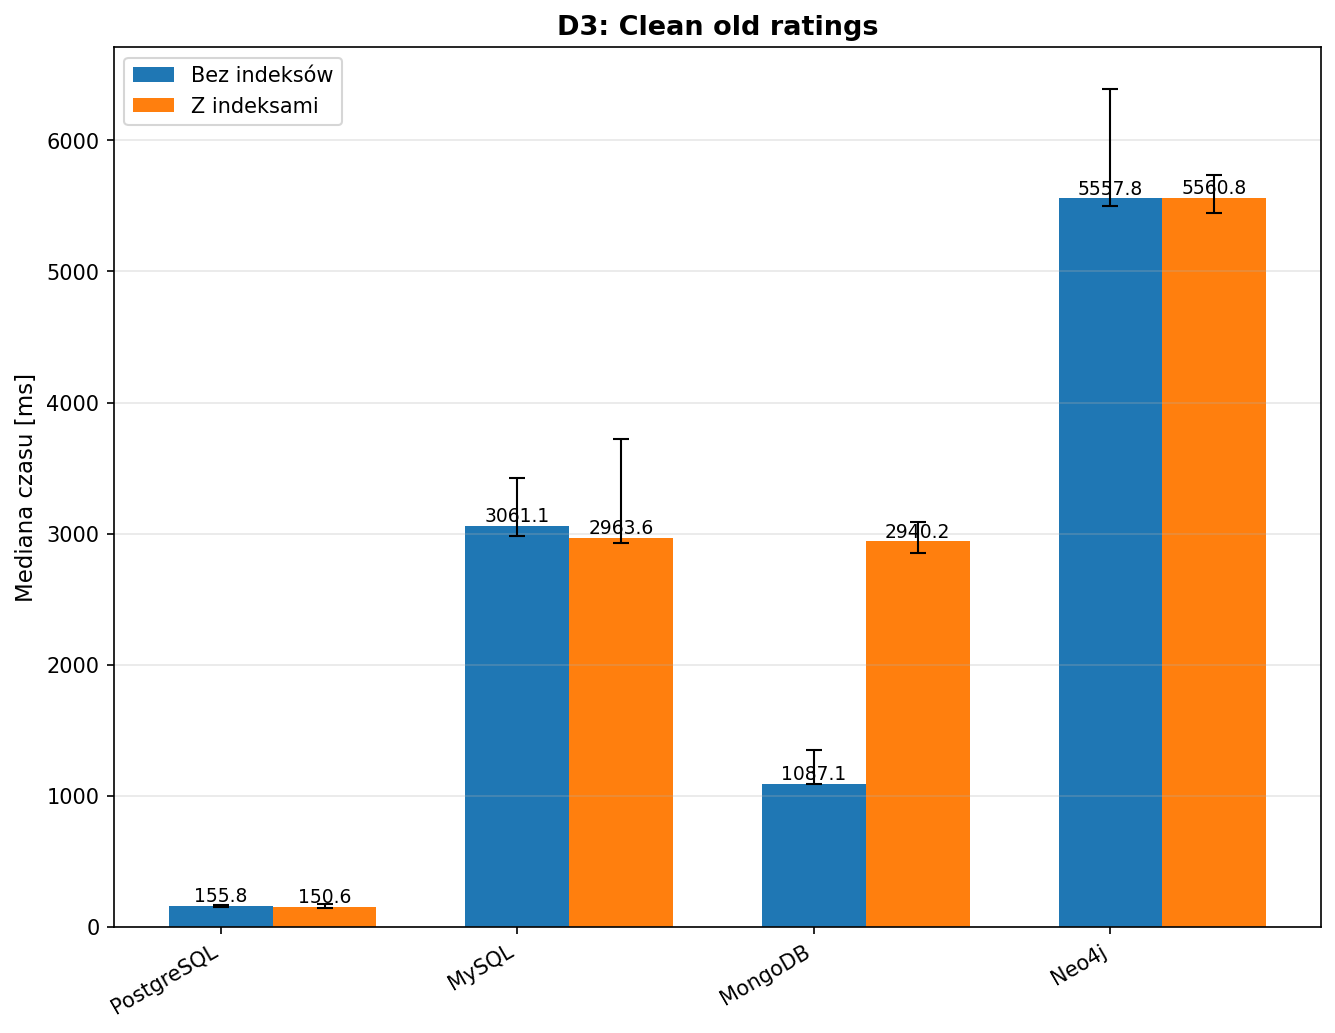
\includegraphics[width=0.8\textwidth]{charts/large/chart_D3.png}
    \caption{D3 -- Czyszczenie starych ocen (large)}
\end{figure}

\subsubsection{D5: Usunięcie subskrypcji z płatnościami}
\begin{figure}[H]
    \centering
    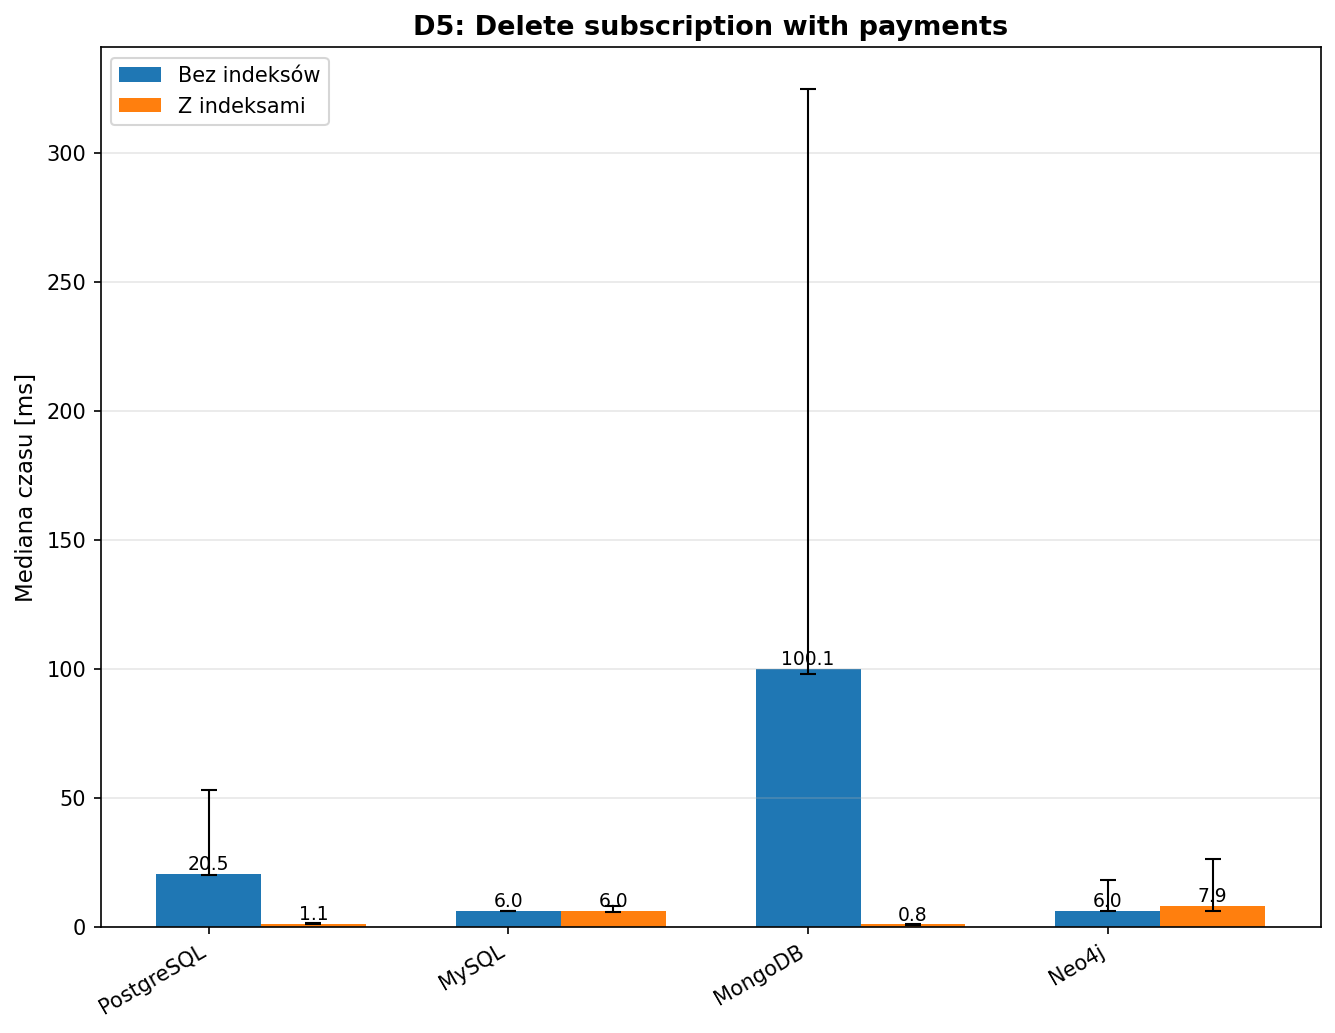
\includegraphics[width=0.8\textwidth]{charts/large/chart_D5.png}
    \caption{D5 -- Usunięcie subskrypcji z płatnościami (large)}
\end{figure}

% -------------------------------------------------------
% UPDATE
% -------------------------------------------------------

\subsubsection{U1: Aktualizacja postępu oglądania}
\begin{figure}[H]
    \centering
    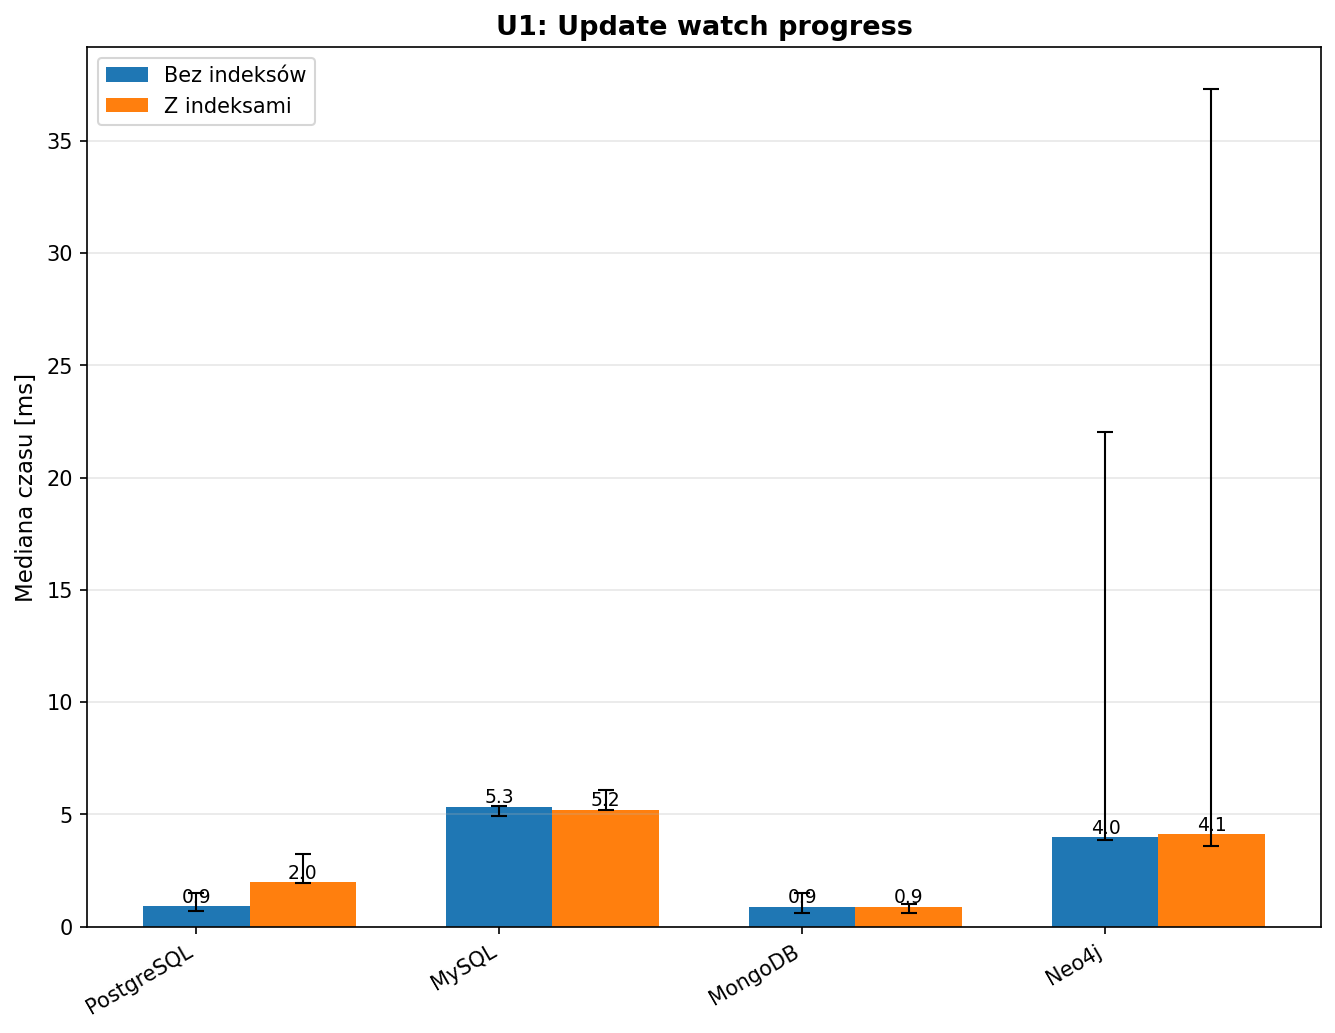
\includegraphics[width=0.8\textwidth]{charts/large/chart_U1.png}
    \caption{U1 -- Aktualizacja postępu oglądania (large)}
\end{figure}

\subsubsection{U4: Aktualizacja danych użytkownika}
\begin{figure}[H]
    \centering
    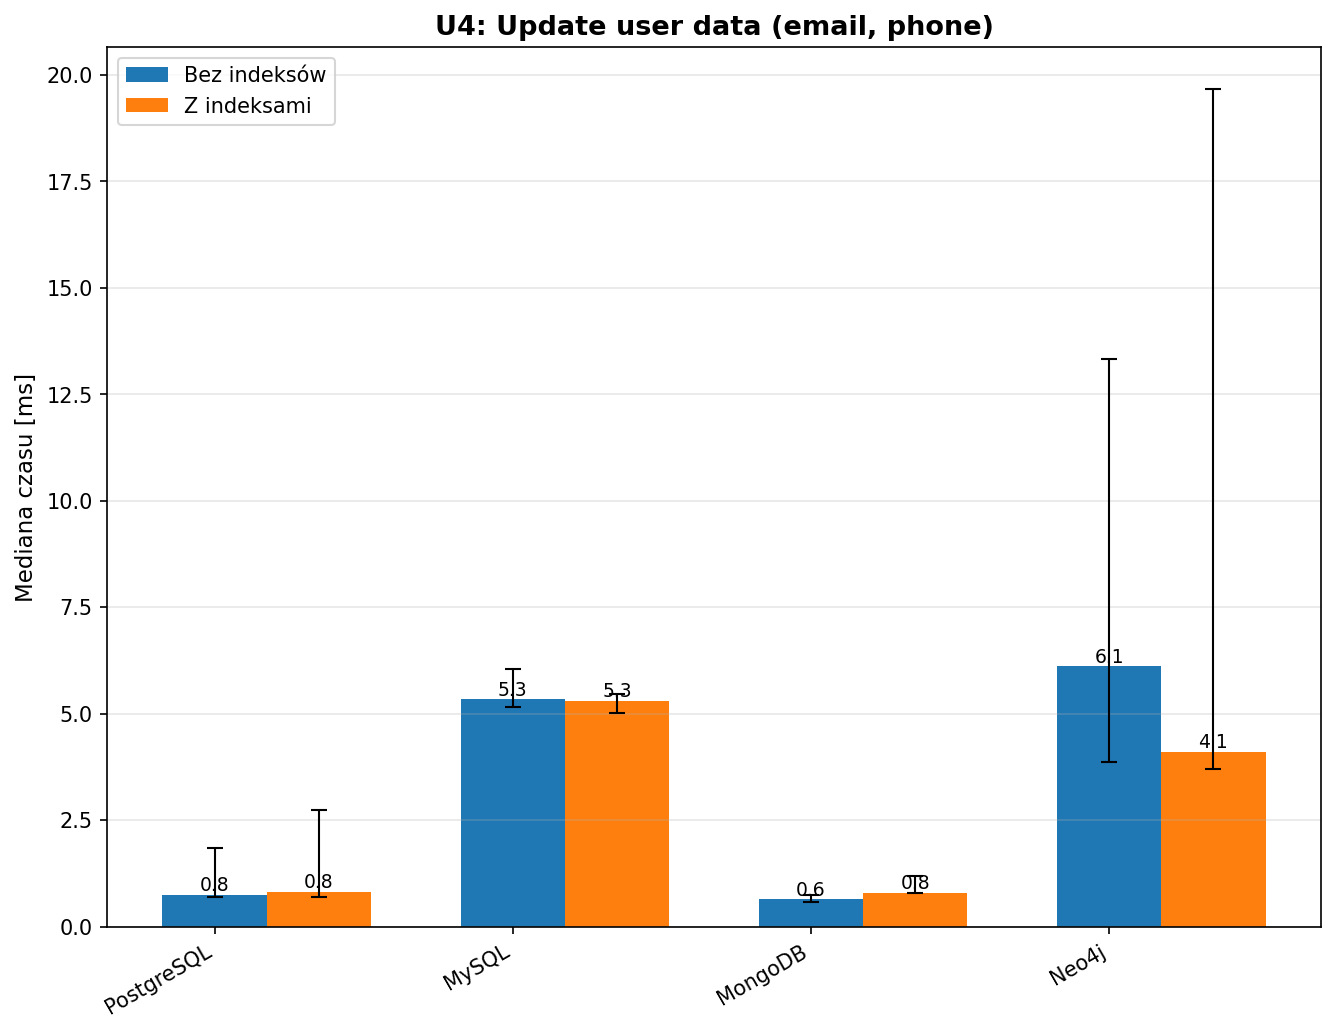
\includegraphics[width=0.8\textwidth]{charts/large/chart_U4.png}
    \caption{U4 -- Aktualizacja danych użytkownika (large)}
\end{figure}

\subsubsection{U5: Oznaczenie treści jako nieaktywnej}
\begin{figure}[H]
    \centering
    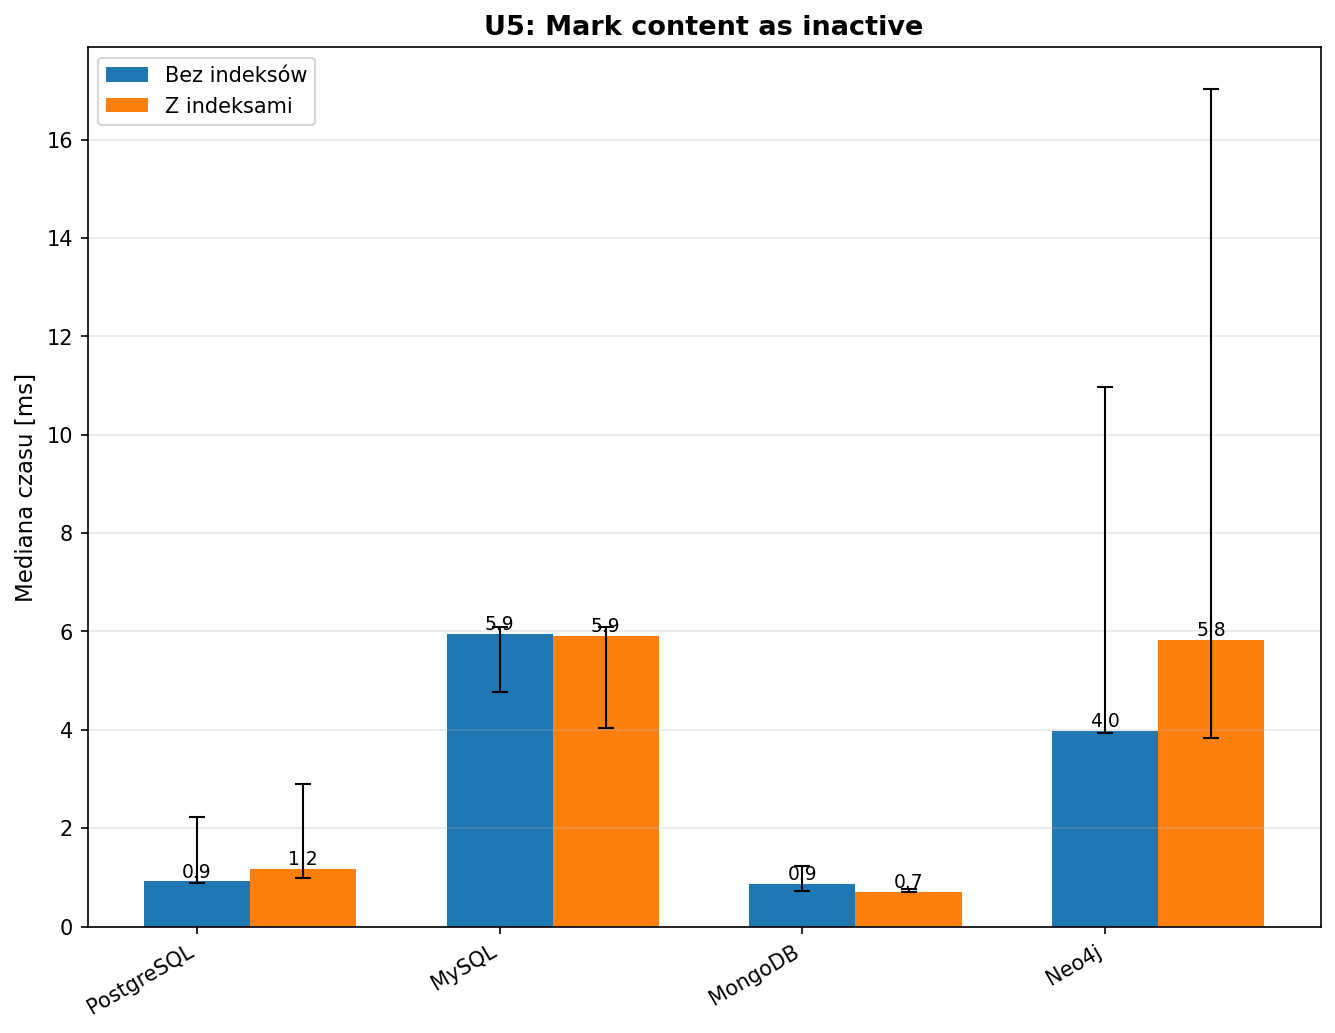
\includegraphics[width=0.8\textwidth]{charts/large/chart_U5.png}
    \caption{U5 -- Oznaczenie treści jako nieaktywnej (large)}
\end{figure}

\subsubsection{U6: Masowa aktualizacja wskaźnika popularności}
\begin{figure}[H]
    \centering
    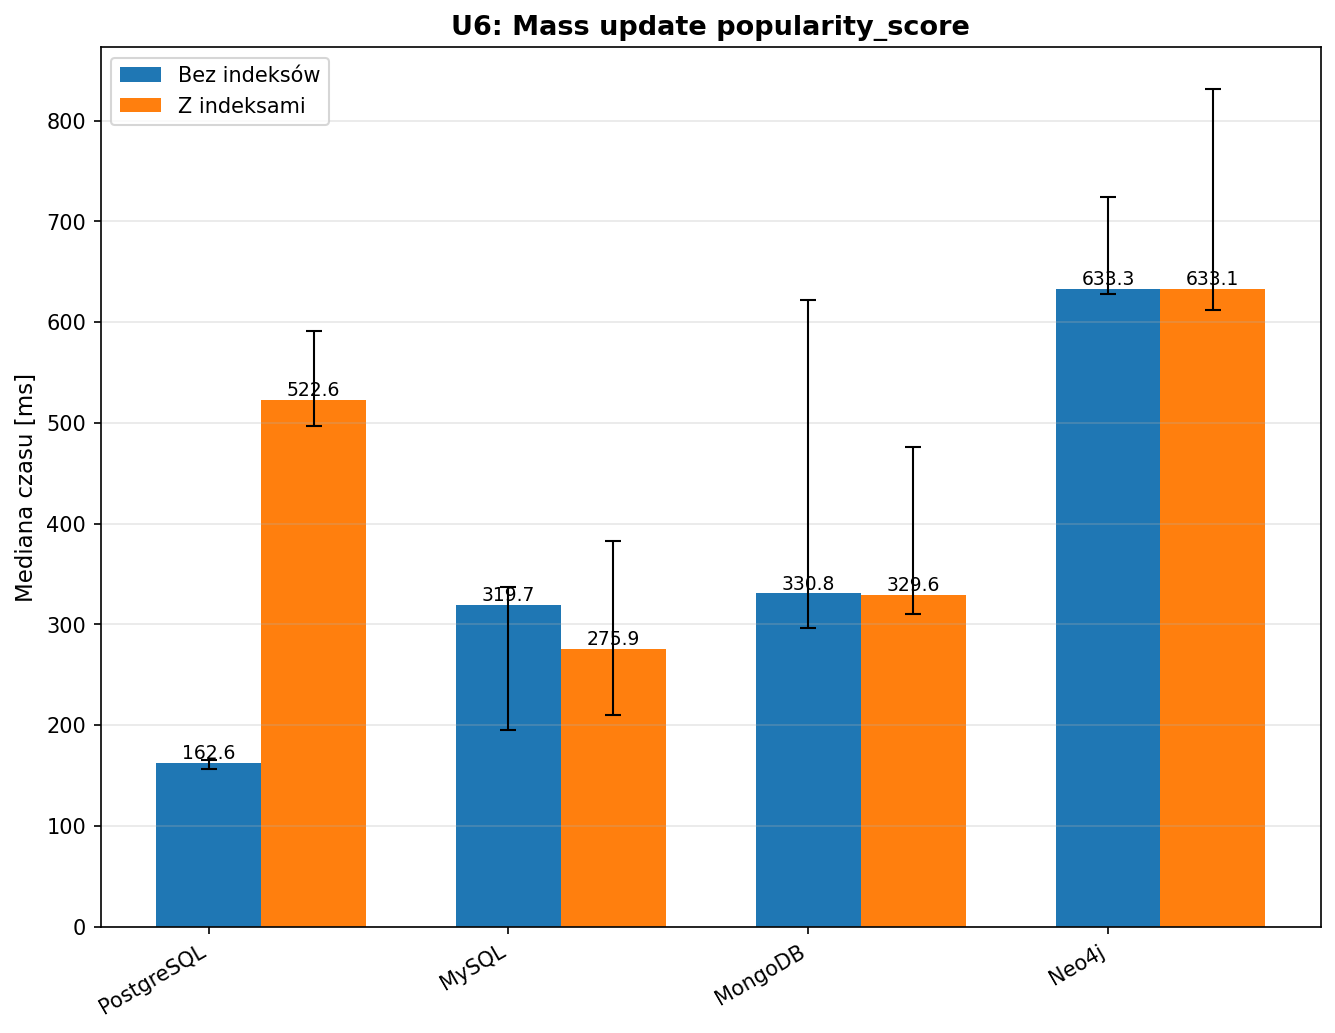
\includegraphics[width=0.8\textwidth]{charts/large/chart_U6.png}
    \caption{U6 -- Masowa aktualizacja wskaźnika popularności (large)}
\end{figure}


\end{document}